\documentclass[11pt,a4paper]{article}
\usepackage[utf8]{inputenc}
\usepackage[german]{babel}
\usepackage[T1]{fontenc}
\usepackage{hyperref}
\usepackage{amsmath}
\usepackage{amsfonts}
\usepackage{amssymb}
\usepackage{graphicx}
\usepackage{listings}
\usepackage[left=2.5cm,right=2.5cm,top=2.5cm,bottom=2cm]{geometry} 
\usepackage{tabularx}
\usepackage{blindtext}
\usepackage{hyphenat}
\usepackage{nameref}
\usepackage{float}
\usepackage{pgfplots}
\usepackage{tikz}
\usepackage{caption}
\usepackage{subcaption}
\usepackage{float}
\usepackage{lineno}
\linenumbers
\usepackage{array}
\usepackage{newclude}
\DeclareUnicodeCharacter{00B0}{~}

\makeatletter
\makeatother

\newcommand{\ms}{\mathrm{ms}}

\newcommand{\bibLabel}[1]{\label{#1}\hypertarget{#1}{}}
\newcommand{\bibRef}[1]{\hyperlink{#1}{$^{[\ref*{#1}{}]}$}}

\newcommand{\productName}{Varroabekämpfungsmechanismus}

\newcommand{\subpicture}[2]{
    \begin{subfigure}{.3\textwidth}
        \centering
        \includegraphics[width=.7\textwidth]{#1}
        \caption{#2}
    \end{subfigure}
}

\begin{document}
\sloppy 			% damit keine langen Wörter über den rechten Rand stehen

\begin{center}
\Large{Spezialschulteil des Albert-Schweitzer-Gymnasiums Erfurt}\\[1.5ex]
\large{Seminarfacharbeit Klasse 11/12}
\end{center}
\normalsize


\thispagestyle{empty}
\vspace*{2cm} % Vertikaler Abstand
\begin{center}

\includegraphics[scale=.4]{images/logo}\\
\vspace*{2cm}
% Titel der Arbeit:
\Huge{\textbf{Entwicklung einer optischen Varroamilbenerkennung auf Bienen und anschließende Bekämpfung}} 

\end{center}
\normalsize

\vspace*{4cm}
\Large{ % Große Schriftgröße
\begin{tabular}{ll}
Fachbetreuer: & Herr Süpke \\
Seminarfachbetreuer: & Frau Nadler \\

Name: & Albert H. Dehne \\
& Daniel F. Cermann\\
& Richard Ueltzen\\

Datum: & \today
\end{tabular}
}
\normalsize % Setzt zurück auf normale Schriftgröße

\newpage

% Inhaltsverzeichnis
\thispagestyle{empty}
\setcounter{page}{1}
\tableofcontents
\newpage


% ---------------------------------------
% ------------Einleitung-----------------       1 Seite
% ---------------------------------------
\section{Einleitung}
Jährlich sterben etwa 15\% der Bienenvölker in Deutschland an den Folgen von Varroamilbenbefall \bibRef{i1}.
Viele weitere Bienenstöcke werden zusätzlich durch den Parasiten stark geschwächt.\\
Dies ist ein großes Problem: Nicht nur für Bienen, sondern auch für Natur und Mensch. Weltweit sind 80\% der Pflanzen auf die Bestäubung von Bienen angewiesen. Die enorme Bedeutung der Bienen spiegelt sich auch im geschätzten Wirtschaftswert der Biene, etwa 265 Milliarden Euro jährlich, wieder \bibRef{i2}.
Aktuell gibt es verschiedene Wege, die Varroamilbe zu bekämpfen. Jedoch sind die meisten dieser Methoden ineffizient \footnote{starke Quelle}. Des Weiteren sind die ökologischen Schäden, welche die Anwendung der gängigen Säurebehandlung nach sich ziehen, nicht zu vernachlässigen. Sie gegen den Nutzen in jedem Falle abgewogen werden. Andere Bekämpfungsmethoden sind unter anderem die Wärmebehandlung von ganzen Bienenstöcken. Diese hat jedoch nur einen Wirkungsgrad von circa 60\%.\\
Wir haben uns zum Ziel gesetzt, eine neue Behandlungsmethode zu entwickeln. Dabei ist uns besonders wichtig, den ökologischen Schaden für die Bienen und die Umwelt so gering wie möglich zu halten. Unser Ziel ist dabei, nur die betroffenen Bienen zu behandeln. Dies wollen wir durch eine optische Erkennung der Varroamilben am Bienenstockeingang ermöglichen. Anschließend sollen befallene Bienen erkannt und abgesondert werden. Nach diesem Prozess kann die betroffene Biene behandelt werden und wieder in den Bienenstock zurückgeführt werden. Dieses Vorgehen ermöglicht darüberhinaus eine ganzjährige Behandlung eines Bienenstocks und hat im Gegensatz zu bisherigen Methoden das Potenzial, das Eindringen der Varroamilben in den Stock präventiv zu verhindern.  Dem gegenüber steht z.B. die Säurebehandlung, welche nur durchgeführt werden kann, wenn die Bienen keinen Nektar sammeln. Unser Hauptziel besteht darin, den erstmaligen Befall mit der Varroamilbe zu verhindern. Eine Kombination von konventionellen Behandlungsmethoden und unserer neuen Mehthode könnte Bienenstöcke vollständig von Milbenbefall befreien.\\
In unserer Arbeit fokussieren wir uns auf die optische Varroamilbenerkennung, um die Grundlage zur Bekämpfung zu schaffen. Des Weiteren können durch die Erkennung des Schädlings Forschungsdaten zum Verhalten von Bienen und Varroamilben kostenkünstig erhoben werden. Die Bekämpfung der Varroamilben arbeiten wir konzeptionell aus und sammeln unsere technischen Umsetzungsideen.\\
An dieser Stelle möchten wir ein Dankeschön für die Unterstützung an unseren Fachbetreuer Johannes Süpke und unsere Seminarfachbetreuerin Dörte Nadler aussprechen. Des Weiteren möchten wir uns in besonderer Weise für die tatkräfte Unterstützung unseres Außenbetreuers Jan Rimbach bedanken, welcher uns stets mir fachkundiger Auskunft zur Seite stand und uns mit der aktuellen Technik ausgestattet hat. Ein weiterer Dank geht an das Schülerforschungszentrum, vertreten durch Frank Paulig. \\




% ---------------------------------------
% ----------Theoriekapitel---------------           2 - 3 Seiten ~ Albert
% ---------------------------------------
\newpage
\section{Die westliche Honigbiene Apis mellifera} \label{section:Theory}

\subsection{Beschreibung der Apis mellfiera}
Die Apis mellifera – umgangssprachlich auch westliche Honigbiene – gehört zur Familie der Echten Bienen. Durch den enormen wirtschaftlichen Nutzen der Apis mellifera wurde durch die Industrialisierung das Verbreitungsgebiet, welches ursprünglich Europa, Afrika und Vorderasien war, erweitert. Durch die Kolonialisierung ist die Apis mellifera heutzutage auf der ganzen Welt verbreitet. Dies führte dazu, dass sich das Parasit Varroa destructor, welcher vorerst nur die Apis cerana als Wirt hatte zu einem der gefährlichsten Parasiten für die westliche Honigbiene.\footnote{Diana Sammataro, Uri Gerson, Glen Needham: Parasitic mites of honey bees, Life history, implications, and impact, in Annual Review of Entomology, Bd, 45, 2000, S. 519–548} \\
Die Apis mellifera ist 11-18 mm groß. Dabei gibt es Unterschiede zwischen Arbeiterinnen, Drohnen und der Königin. Die westliche Honigbiene hat eine braune Grundfarbe. Die Apis mellifera besitzt, wie alle Insekten einen Außenskelett aus Chitin. Die Biene ist in drei Abschnitte unterteilt: Kopf, Thorax und Abdomen. \footnote{\url{https://www.lernhelfer.de/schuelerlexikon/biologie/artikel/honigbiene}, letzter Zugriff am 17.12.2021}
% Verwies auf Abbildung im Anhang
\subsection{Bedeutung der Apis mellifera}
Die westliche Honigbiene hat eine enorme ökologische, als auch wirtschaftliche Bedeutung. Die Apis mellifera ist für die Bestäubung von fast 80\% aller Nutz- und Wildpflanzen verantwortlich. "Von 100 Pflanzenarten, die über 90 Prozent der Nahrung der Menschen sicherstellen, werden Beobachtungen zufolge 71 von Bienen bestäubt." \footnote{\url{https://www.bee-careful.com/de/initiative/warum-sind-bienen-so-wichtig/}, letzter Zugriff am 17.12.2021} Die führt zu einer Wertschöpfung der westlichen Honigbiene von 265 Milliarden Euro pro Jahr. Zudem ist die westliche Honigbiene maßgebliche für die Pflanzenvielfalt in ihrem Verbreitungsgebiet verantwortlich.  

\section{Die Milbe Varroa destructor}

\subsection{Geschichtlicher Überblick}
Die Milbe Varroa destructor wurde im Jahr 1904 zum ersten Mal auf einer östlichen Honigbiene – Apis cerana, auch Apis indica – entdeckt. Anschließend wurde sie im gleichen Jahr von Oudemans beschrieben und klassifiziert. Er benannte sie nach ihrem Entdecker Eward Jacobson. Dadurch entstand der Name Varroa jacobsoni. Erst später wurde entdeckt, dass zwei sehr ähnliche Milben unter dem gleichen Namen beschrieben wurden. Anfang der Zweitausender wurde endgültig eine Unterscheidung in die Milbe Varroa jacobsoni und die Milbe Varroa destructor vorgenommen \footnote{\url{http://www.mellifera.ch/cms/index.php/news/varroa-jacobsoni-westliche-honigbiene} letzter Zugriff am 16.12.2021}. Unsere gesamte Arbeit behandelt hierbei die Milbe Varroa destructor. \\
Die Milbe Varroa destructor war zum Anfang des 20. Jahrhunderts auf das Ausbreitungsgebiet der Apis cerana beschränkt, welches die gesamte östliche Hemisphäre bis zur Linie Ural/Afghanistan beinhaltet. Dies erklärt auch ihre erste Entdeckung auf der indonesischen Insel Java. Für einen langen Zeitraum gab es bis auf ein paar wenige Beschreibungen kaum Meldung über die Milbe. Sie galt als harmloser Parasit der Apis cerana. 
Durch die zunehmende Industrialisierung gegen Ende der 1950er Jahre entstand eine Durchmischung der asiatischen Honigbiene Apis cerana und der europäischen Apis mellifera. Die führte dazu, dass die Milbe Varroa destructor von der östlichen auf die westliche Honigbiene übergehen konnte. Die Varroa destructor und die Apis cerana haben sich im Laufe der Zeit aufeinander eingestellt und ein gesundes Wirt – Parasit Verhältnis entwickelt, welche für beide das Überleben sicherten. Da diese Zeit beim plötzlichen Übergriff auf die Apis mellifera fehlte, waren tausende Völker schwer geschädigt. Zu diesem Zeitpunkt Anfang der 1950er Jahre wurden unter anderem in der damaligen UdSSR umfangreiche Untersuchung über die Erkrankungen der Apis mellifera Völker angestellt. Allerdings bliebe diese ohne Erfolg und man identifizierte die Milbe Varroa destructor nicht als den Auslöser. Die Erkenntnis über den Zusammenhang zwischen der Erkrankung von Apis mellifera Völkern und dem Befall mit Varroa destructor erbrachte erst 1958 der chinesische Forscher Ian Tzin-He. \footnote{Eva Rademacher, Erika Geiseler: Die Varroatose der Biene, Gesichte, Diagnose, Therapie, 3. überarb. Auflage, Berlin, Schelzky und Jeep, 1986, Seite 8ff.}

\subsection{Beschreibung des Parasiten}
Nach aktuellem Stand sind vier Arten von Varroamilben bekannt. Neben der bereits erwähnten Varroa jacobsoni, welche man lange Zeit für die Hauptursache des Bienensterbens ansah gibt es noch Varroa underwoodi (Delfinado-Baker und Aggarwal 1987) und die Varroa rinderi (De Guzman und Delfinado-Baker 1996). Erst im Jahr 2000 entdeckte man durch mitochondrialer-DNA-Analysen, dass es sich bei der Varroa jacobsoni um einen Komplex aus zwei Milbenspezies handelt. Die neu Entdeckte Art Varroa destructor lässt sich wie folgt klassifizieren: \footnote{\url{https://edoc.ub.uni-muenchen.de/12025/1/Schneider_Verena.pdf} letzter Zugriff am 16.12.2021}\\
\begin{center}
\begin{tabular}{l|l}
     Stamm & Arthropoda \\
     Klasse & Archnidae  \\
     Ordnung & Acari \\
     Unterordnung & Mesostigmata \\
     Familie & Dermanyssidae \\
     Gattung & Varroa. \\
\end{tabular}\\
\end{center}
Der Körper der Varroa destructor ist in zwei Teile untergliedert (siehe Anhang S. ---). Die Idiosoma stellt den eigentlichen Körper mit den Beinen dar. Die Gnathosoma ist der Bereich der Mundwerkzeuge. 
Die weibliche Milbe ist rotbraun und hat eine querovale Form. Sie ist ca. 1,1x1,6mm groß. Die Idiosoma besitzt eine harte Kutikula. Diese bildet auf dem Rücken der Milbe einen Schild. Auf dem Buch laufen häutige Chitinplatten zusammen. Die Kutikula ist stark mit Borsten besetzt. Diese dienen der Milbe zum festen Halt im Fell der Biene. Auf der anderen Seite bieten sie auch eine elastische Hülle, damit die Milbe in einer Bienenzelle nicht zwischen der Brut und der Zellwand anheftet. Die Milbe hat 8 Beine, von denen sich vier auf der Unterseite befinden. Diese vier Beine haben ein besonders stark ausgebildetes Haftorgan. 
Die Gnathosoma ist beweglicher mit der Idiosoma verbunden. Nach Smirnow schlagen bei der Nahrungsaufnahme die Mundwerkzeuge ein Loch durch die Bienenhaut und kommen somit an die Hämolymphe, das Bienenblut. Dies saugen die Milben durch ihre gut herausgebildete Muskulatur im Mundbereich heraus. 
Die männlichen Milben sehen den weiblich nicht ähnlich. Sie sind fast weiß, rundlicher und ca. 0,8mm groß. Im Gegensatz zu den Weibchen haben sie eine recht dünne Kutikula, welche auch kaum mit Borsten besetzt ist. Ihre Mundwerkzeuge dienen eher als Hilfsorgane für die Begattung, weshalb ausgewachsene männliche Varroamilben nicht als Parasiten zählen, da sie nicht die Möglichkeit haben die Hämolymphe aus den Bienen zu sagen.
Die Varroamilben verfügen über ein Nervensystem, welches eine gehirnähnliche Struktur aufweist. \footnote{Eva Rademacher, Erika Geiseler: Die Varroatose der Biene, Gesichte, Diagnose, Therapie, 3. überarb. Auflage, Berlin, Schelzky und Jeep, 1986, Seite 22ff.}

\subsection{Verbreitung des Parasiten}
In China wurde die Milbe Varroa destructor erstmals 1958 auf einer Apis mellifera festgestellt. In den anschließenden Jahren folgten weitere Sichtungen in verschiedenen Ländern. So wurde 1964 offiziell eine Milbe in der damaligen UdSSR identifiziert. Dies geschah am gleichen Ort, wo Jahre zuvor schon Untersuchungen aufgrund enormes Bienensterbens, welche durch die Milbe ausgelösten wurden, untersucht worden waren. Anschließend breitete sich die Varroamilbe über das heutige Russland von Osten und Richtung festen schnell aus. Vorerst gab es keine größeren Bedenken wegen des neuen Parasiten und frühe Kongresse zum Thema Varroamilben waren schlecht bezahlt. Jedoch breitete sich die Milbe über rasanter aus und eroberte in Rekordzeit Europa. Um den enormen Bienensterben entgegenzuwirken, gab es mehrere großangelegte Bekämpfungsaktionen. So wurden. So wurden im Zeitraum von 1980-1983 in der damaligen ČSSR 30.000 Völker vernichtet. Der Befall wurde dadurch jedoch nicht gestoppt. Heute ist die Milbe Varroa destructor auf allen Kontinenten mit Ausnahme von Australien vorzufinden (siehe Anhang S. ---. \footnote{Eva Rademacher, Erika Geiseler: Die Varroatose der Biene, Gesichte, Diagnose, Therapie, 3. überarb. Auflage, Berlin, Schelzky und Jeep, 1986, Seite 10ff.}

\subsection{Krankheitsverlauf durch Befall des Parasiten}
Der Befall eines Bienenstockes durch die Milbe Varroa destructor führt zu schweren Schäden. Dabei unterscheidet man den Befall der Bienenbrut und den Befall vollständig entwickelten Bienen. Die Milben befall Bienenlarven und saugen deren Hämolymphe. Die führt zu einem Gewichtsverlust je nach Anzahl der Milben, welche eine Larve befallen von bis zu 25\%. Dies entspricht einen Blutverlust von bis zu 40\%. Die Folge des Befalls und des Blutverlustes ist, dass die Larven sich nicht richtig entwickeln können. Dies führt wiederum zu einer drastisch kürzeren Lebenserwartung. Des Weiteren kann ein besonders starker Befall durch den Parasiten dazu führen, dass die Biene nur sehr bedingt lebensfähig ist. Sie haben oft Missbildungen und werden deshalb aus dem Stock entfernt.
Bei einem Befall von Erwachsenen Bienen treten andere Phänomene auf. Die Biene wird durch den Befall verunsichert und probiert durch intensives Putzen die Milbe loszuwerden. Dies gelingt ihr aber nicht. Die Folgen sind nun ähnlich wie bei der Brut. Die Milben saugen Blut aus der Biene, was diese schwächt. Außerdem kommen Faktoren, wie das zusätzliche Gewicht durch die Milbe, welches ungefähr 1/30 ihres Gesamtgewichtes ausmacht hinzu. Dies führt zu eine beeinträchtigen Flugfähigkeit. Letztendlich führen alle diese Faktoren dazu, dass die Biene nicht mehr ihren eigentlichen Aufgaben innerhalb des Volkes zu 100\% nachgehen kann. Letztendlich führt die Einstichstelle der Milben dazu, dass eine Sekundärinfektion auftritt, welche zu Tod der Biene führt. \\
Auf lange Sicht wird ein Bienenvolk enorm geschwächt und sofern das Volk nicht behandelt wird, so wird es in jedem Falle zu Grunde gehen. \footnote{Eva Rademacher, Erika Geiseler: Die Varroatose der Biene, Gesichte, Diagnose, Therapie, 3. überarb. Auflage, Berlin, Schelzky und Jeep, 1986, Seite 31ff.}


\subsection{Herkömmliche Bekämpfungsmethoden}
Zur Bekämpfung des Parasiten Varroa destructor werden zahlreiche verschieden Methoden eingesetzt. Die effektivsten sind hierbei die Behandlung eines Bienenstockes mit chemischen Mitteln. Weniger effektive, dafür umweltfreundlicher sind verschiedene physikalischen und biologische Methoden.

\subsubsection{Chemische Mittel}
Häufig werden chemische Mittel gegen die Varroamilbe eingesetzt, die schon Anwendung in der Pflanzenbehandlung gefunden haben. Bei chemischen Mitteln ist immer darauf zu achten, dass der Schaden groß genug ist, um die Milbe zu bekämpfen und klein genug, um die Biene nicht zu stark zu schädigen. Dies führt dazu, dass die meisten chemischen Mittel wie z.B. Ameisensäure und Oxalsäure nur eingesetzt werden dürfe, während die Bienen noch keinen Nektar sammeln, um die Brut und den Honig nicht zu schädigen. Chemischen Mittel können einen Wirkungsgrad von bis zu 90\% erreichen. Wirkungsgrade nahe der 90\% und über 90\% sind aber nur bei einer durchgehenden Behandlung zu erwarten, was längerfristig dem Bienenvolk enorm schadet und davon abgesehen werden sollte. Besonders gute Wirkstoffe, wie der Wirkstoff Folbex VA neu, welcher 1982 zugelassen wurde, versprachen sehr hohe Wirkungsgerade, wurden jedoch später aufgrund von Rückständen in Honig verboten.\footnote{Eva Rademacher, Erika Geiseler: Die Varroatose der Biene, Gesichte, Diagnose, Therapie, 3. überarb. Auflage, Berlin, SChelzky und Jeep, 1986, Seite 46ff.}
\subsubsection{Physikalische und biologische Methoden}
Eine physikalische Methode zur Bekämpfung des Parasiten ist die Wärmebehandlung. Bei 46-48°C sterben die Varroamilben ab. Bei geringfügig höherer Temperatur sterben jedoch auch die Bienen ab, weshalb diese Methode keine breite Anwendung findet. 
Biologische Methoden sind zum Beispiel der Einsatz von varroapathogenen Pilzen, Bakterien oder Viren. Hier wurden jedoch noch keine Praxistauglichen Methoden entwickelt. Jedoch werden verschiedene biotechnischen Maßnahmen eingesetzt, wie zum Beispiel spezielle Waben, die den Varroabefall mildern sollen. Die Wirkungsgrade solcher Methoden sind nicht besonders hoch. \footnote{Eva Rademacher, Erika Geiseler: Die Varroatose der Biene, Gesichte, Diagnose, Therapie, 3. überarb. Auflage, Berlin, SChelzky und Jeep, 1986, Seite 62ff.}



% ---------------------------------------
% ----------Vorbetrachtungen-------------           2 - 3 Seiten ~ Daniel
% ---------------------------------------
\newpage
\section{Vorbetrachtungen und Experimente} \label{section:Vorbetrachtungen}

% $\rightarrow$ mögliche Lösungsansätze\\
% $\rightarrow$ Mit Experimenten flexen\\

\subsection{Aufbaumöglichkeiten der Varroaerkennung}
Wir starteten den Entwicklungsprozess mit einem Austausch unserer Vorstellungen. Durch ein Brainstorming trugen wir verschiedene Ideen, technische Ansätze und Anforderungen an das Milbenerkennungssystem zusammen. \\
Ein erster Ansatz war, die Bienen mit Kameras zu filmen und somit die Milben optisch zu erkennen. Durch Anpassung der äußeren Bedingungen, wie Lichtverhältnisse, wollten wir die Erkennung so zuverlässig wie möglich gestalten.\\
Eine weitere Idee beruht auf einer möglichen Wärmedifferenz zwischen Bienen und Milben: Wäre die Differenz der Körpertemperaturen gut messbar, könnten wir beim Filmen mit Wärmebildkameras vermutlich Milben als warme bzw. kalte Punkte auf den Bienen erkennen. Diese Methode hätte allerdings beträchtliche Nachteile: Zum einen sind Infrarot-Kameras mit der von uns benötigten Auflösung sehr teuer. Unsere Varroamilbenerkennung würde also auch langfristig nicht preiswert sein und somit keine weitreichende Anwendung finden. Außerdem sind Bienen wechselwarm\bibRef{wechselwarm}. Die stark von der Außentemperatur abhängenden Schwankungen der Körperkerntemperatur würden wahrscheinlich zu Ungenauigkeiten und ungeahnten Problem bei der Milbenerkennung führen.\\
Auch andere Möglichkeiten, die wir in Betracht zogen, hatten große Nachteile oder waren mit unseren Mitteln nicht umsetzbar. Also kamen wir zu dem Schluss, das Erkennen der Milben mit Kameras durchzuführen.\\
Nach unserer ersten Abwägung von Ideen war der nächste Schritt, das Scannen der Bienen konzeptionell zu planen. Alle unserer Überlegungen beruhten dabei auf einem von zwei grundsätzlichen Ansätzen: Entweder jede Biene wird durch Bewegung der Kamera bzw. Veränderung des Zooms einzeln fokussiert und anschließend auf Varroen gescannt oder eine Kamera ist statisch und überwacht gleichzeitig mehrere Bienen aus ihrem Sichtfeld. Bei der Entscheidung für eine Herangehensweise, mussten wir Klarheit und Auflösung der Bilder gegen Kosten und Aufwand abwägen.\\
Der erste der beiden Ansätze hatte den großen Vorteil, dass die Auflösung der fotografierten Biene höher wäre. Versuche von uns haben gezeigt, dass ein kleinerer Abstand der Kamera zur Biene für einen hohen Kontrast der Milben sorgt und somit auch für die Varroaerkennung, unabhängig von der verbesserten Auflösung, förderlich ist. Allerdings brächte man für eine Durchführung dieser Idee in jedem Fall mechanische Vorrichtungen. Die Skizze einer möglichen Umsetzung mit auf linearen Achsen montierten Spiegeln ist im Anhang auf Seite \pageref*{fig:technical-sketch} \, zu erkennen.\\
Neben den theoretischen Überlegungen führten wir außerdem Tests mit Servomotoren durch. In einem einfachen, 3D-gedruckten Versuchsaufbau testeten wir wie schnell die Kamera auf beliebige Stellen des Flugbretts geschwenkt werden kann (siehe Anhang S. \pageref*{fig:mechanics-test}\,). Die Versuche ergaben, dass wir pro Sekunde etwa eine Biene untersuchen könnten. Natürlich ließe sich diese Rate verbessern. Angesichts der Anforderung im Sommer bis zu als 20 Bienen pro Sekunde erkennen zu können, häuften sich die Argumente trotz dessen gegen diese Idee. Bei Abschätzungen der Kosten, Geschwindigkeitslimitierenden Faktoren, Lautstärke und Wartungsaufwand des Systems entschieden wir uns schließlich ganz gegen diesen Ansatz.\\
Das zweite Konzept ist in der Umsetzung rein vom Versuchsaufbau um einiges leichter. Trotzdem mussten wir vor der Umsetzung einige Optionen abwägen. Beispielsweise mussten wir entscheiden, ob viele billige Kameras, die jeweils nur einen kleinen Bereich des Flugbretts überwachen oder wenige Kameras mit einer sehr hohen Bildqualität und Auflösung bessere Resultate erzielen werden. Wir kamen zu dem Ergebnis, dass das zweitere die bessere Option ist. Unsere Überlegungen dazu sind im Anhang auf Seite \pageref*{fig:moving-cameras-considerations} \, nachzuvollziehen.\\
Eine weitere, besonders schwierige Frage, die sich uns stellte, war, ob wir neben der Oberseite auch die Unterseite der Bienen durch Kameras untersuchen sollten. Dazu wären mehr Kameras nötig und das Flugbrett müsste aus einem durchsichtigem Material, zum Beispiel Plexiglas, sein. 	Aufgrund des ungemein größeren Aufwands, der großen Veränderung des Einflugbereichs von den Bienen und der Tatsache, dass Milben hauptsächlich auf dem Rücken der Bienen sitzen haben wir uns gegen weitere Kameraperspektiven.\\
Schlussendlich war unsere gewünschte Kamerakonfiguration wie folgt: Zwei Kameras filmen jeweils eine Hälfte des Flugbretts zentral von oben. Nur in der Mitte des Brettes überlappen sich die Bilder etwas.

\subsection{Experimente zur Optimierung der Fotoqualität}
Um Varroamilben möglichst zuverlässig auf Bienen zu erkennen, muss der Kontrast zwischen Milbe und Biene so ausgeprägt wie möglich sein. Durch Durchführung systematischer Experimente haben wir die Rahmenbedingungen für ein solches Optimum so präzise wie möglich festgestellt.\\
Bei allen durchgeführten Versuchen fotografierten wir tote Bienen, auf deren Rücken oder Panzer eine Varroamilben saß. Dabei haben wir von außen kommendes Licht fast vollständig abgeschirmt, um zufällige Fehler durch Sonnenlicht oder andere Beleuchtungen zu vermeiden. Somit hatten wir die Möglichkeit alle Bedingungen eines Fotos nahezu konstant zu halten und nur einen Einfluss gezielt zu verändern.\\
Bei unseren Untersuchten beschränkten wir uns speziell auf die optimale Helligkeit und Wellenlänge der Belichtung, sowie die beste Beschaffenheit und Farbe des Untergrunds.\\
\begin{figure}[H] \label{fig:experiment}
        % meine fancy Funktion :)
	\centering
        \subpicture{images/575nm.jpg}{575nm}
        \subpicture{images/595nm.jpg}{595nm}
        \subpicture{images/660nm.jpg}{660nm}
        \subpicture{images/700nm.jpg}{700nm}
        \subpicture{images/770nm.jpg}{770nm}
        \subpicture{images/850nm.jpg}{850nm}
        \subpicture{images/870nm.jpg}{870nm}
        \subpicture{images/925nm.jpg}{925nm}
        \subpicture{images/940nm.jpg}{940nm}
	% \caption{Testbilder bei verschiedenen Wellenlängen}
\end{figure}
\noindent
Die Ergebnisse unserer Versuche bezüglich der optimalen Wellenlänge der Beleuchtung waren eindeutig. Die Milben sind bei Licht mit einer besonders hohen Wellenlänge am besten zu erkennen (siehe Abbildung \ref*{fig:experiment} \,) Bei grünem, orangenem und hellrotem Licht ist der Parasit nur umrissartig oder sogar gar nicht zu erkennen. Im starken Gegensatz dazu hebt sich die Milbe bei dunkelrotem und infrarotem Licht stark als weißer Fleck auf der Biene ab.\\
Die Wellenlänge sollte also zwischen 900 nm und 950 nm liegen, was kurzwelligem Infrarotlicht entspricht. Höher darf die Wellenlänge der Beleuchtung nicht sein. Denn gängige Fotosensoren, Objektive und Linsen sind für sichtbares Licht optimiert. Außerhalb eines Toleranzbereiches bräuchten wir für scharfe Bilder spezielle, teure Optik.\\
Infrarotes Licht wird zudem von Bienen nicht gesehen. Bienen nehmen nämlich Licht nur bis zu einer Wellenlänge von etwa 650nm wahr. Im Anhang auf S. \pageref*{fig:bee-vision} \, ist das für Bienen sichtbare Spektrum zu sehen. Eine Beleuchtung mit Infrarotem Licht können wir also benutzen, ohne die Bienen einzuschränken.\\
Bei den Experimenten zum Untergrund ergab sich, dass Reflexionen und Streuungen des Lichts den Kontrast zwischen Milbe und Biene verschlechtern. Der beste Untergrund sollte somit schwarz sein und möglichst wenig reflektieren.
% nicht so aprupt abbrechen


% ---------------------------------------
% --------------Prototype----------------           3 Seiten ~ Daniel
% ---------------------------------------
\newpage
\section{Entwicklung und Verbesserung verschiedener Prototypen} \label{section:Prototypen}
\subsection{Angewandte Arbeitsmethoden}
Die wohl wichtigste von uns angewandte Arbeitsmethode ist das Rapid-Prototyping. Diese Arbeitsmethode ist ein Verfahren zum Annähern an angestrebte Ergebnisse mittels aufwandsarmer, günstiger Testversionen \bibRef{protoyping}. Wir kamen durch den Bau unserer Prototypen und durch das ständige Ausbessern von Fehlern unserem Ziel, einer immer funktionalen Milbenerkennung, immer näher. Unwichtige Details und ablenkende, kleinere Probleme können bei diesem Prozess vorerst ignoriert werden. Der Fokus auf die wesentlichen Herausforderung kann somit bei der Entwicklung erhalten bleiben. Wir haben beispielsweise Witterungsbeständigkeit erst bei späteren Versionen und Kostenoptimierung bisher gar nicht beachtet.\\
Prototyping ist bei unserem Projekt besonders nützlich, da bei der Arbeit mit Bienen viele Fehlerquellen sehr schwer vorhersehbar sind. Einige Verhaltensweisen der Bienen, vor allem Reaktionen auf Änderungen ihrer Umgebung, sind sehr ungewöhnlich. Bei einem unserer frühen Versionen hatten wir einen zu großen Kasten vor den Eingang des Bienenstocks gebaut. Daraufhin haben die Bienen das Flugloch nicht mehr gefunden und haben sich stattdessen auf dem Flugbrett-ähnlichen Dach unseres Prototypen gesammelt. Hätten wir unser Produkt ausschließlich theoretisch durchgeplant und nicht frühzeitig getest, wären Fehler, wie dieser erst sehr spät aufgefallen.\\
Wir wussten zu Beginn unserer Arbeiten nicht, wie genau ein mögliches Endprodukt aussehen könnte. Durch das Herstellen von Prototypen konnten wir auch alle unsere Lösungsansätze testen. Wir konnten sehr viele vage Ideen schnell umsetzen und immer weiter konkretisieren.\\
Für diese Arbeitsweise war das Arbeiten mit den uns zur Verfügung stehenden 3D-Druckern sehr unersetzbar. Die Kombination aus einem Drucker und Computer-gestütztem Design ermöglichte sehr schnelle Umsetzung von Ideen. Wir nutzten das CAD-Programm ,,Autodesk Fusion 360''. Dieses ist auch für umfangreichere Projekte geeignet und bietei vielseitige Werkzeuge, wie das Simulieren physikalischer Eigenschaften schon vor dem Druck, was den Entwicklungsprozess stark vereinfacht. \\
Schnelles Feetback bekamen wir auch, weil wir direkten Zugriff zu mehreren Bienenvölkern hatten. Dadurch konnten wir auch dynamischer auf entstehender Probleme reagieren und schon früh besonders schwer umzusetztende Ansätze identifizieren.

\subsection{Technische Grundlagen} 
Bevor wir überhaupt die Möglichkeit hatten, Prototypen zu bauen und zu testen, mussten einige Grundgegeben sichergestellt werden.\\
Zum einen brauchten wir eine stabile Stromquelle für Langzeittests. Denn bei den uns zur Verfügung stehenden Bienenkästen ist keine Zugang zum Stromnetz möglich. Eine zuverlässige Stromversorgung zu gewährleisten ist in unserem Fall eine große Herausforderung und war anfangs lange Zeit eine Fehlerquelle von einigen Problemen. Denn die bereitzustellende Leistung ist Zeitweise, immer wenn gerade eine Milbe erkannt wurde, sehr groß. Zu dem ständigen Stromverbrauch des Einplatinencomputers, der Kameras und der Beleuchtung kommen bei der Entdeckung einer Varroamilbe die Last von zwei Servo-Motoren, einem Laser und einer Festplatte zum Aufzeichnen der Daten. So können unseren Abschätzungen zufolge temporär bis zu 20W benötigt werden. Da alle gängigen Einplatinencomputer mit einer Eingangsspannung von $U_{Ges} = 5V$ arbeiten, ist der fließende Strom beträchtlich:
$$ P = U_{Ges} \cdot I \Longleftrightarrow I = \dfrac{P}{U_{Ges}} \approx \dfrac{20W}{5V} = 4A$$
Bei so einer hohen Stromstärke geht selbst bei kleinem Innenwiderstand der Kabel und Steckverbindungen eine hohe Verlustleistung in Form von Wärme verloren. Schon bei einem Innenwiderstand von lediglich $R_i = 0.1\varOmega$ ist dieser Effekt bemerkbar. Unter der Annahme diesen Widerstands des Kabels würde dort die Spannung $U_i$ mit
$$R_i = \dfrac{U_i}{I} \Longleftrightarrow U_i = R_i \cdot I \approx 0.1\varOmega \cdot 4A = 0.4V$$
abfallen. Das bedeutet auch, dass ein zu niedrige Versorgungsspannung an den Komponenten unseres Aufbaus ankommt und unvorhersehbare Effekte auslöst. Das Jetson Nano, das schließich von uns gewählte Baord zur Auswertung der Kamerabilder, drosselt beispielsweise die Rechenleistung oder schaltet bei zu niedrigen Eingangsspannungen das Board ganz ab.\\
Nachdem wir die Spannungsversorgung als Fehlerquelle identifizert hatten, konnten wir durch Verbesserung aller Löt- und Steckverbindungen das beschriebene Problem beseitigen. 
Als Energiespeicher brauchten benutzen wir eine alte Autobatterie. Mit einer Spannung von 12V und einer Kapazität von etwa 50 Amperestunden sollte diese bei einem durchschnittlichem Verbrauch von höchstens 15W länger als 40 Stunden halten. Die Batterie wir durch eine 20W Solarzelle aufgeladen. Außerdem wird die 12 Volt Ausgangsspannung der Batterie durch einen Spannungswandler auf die für von Einplatinencomputer benötigten 5 Volt heruntergewandelt. Der gesamte Aufbau der Stromversorgung ist im Anhang auf Seite \pageref*{fig:power-supply-complete} \, zu erkennen.\\
Eine weitere Grundvorraussetzung für leichten und schnellen Zugriff auf den Varroabekämpfungsmechanismus war eine WLAN-Verbindung im Garten. Besonders für den Entwicklungsprozess ist es wichtig, ohne physische Verbindung auf das Board zugreifen zu können. Auf diese Weise konnten wir per SSH-Verbindung auf den Einplatinencomputer zugreifen. SSH, kurz für ,,Secure Shell'', ist ein kryptographisches Protokoll durch das Entwickler Zugang zu Kommandozeilen von entfernten Servern oder Computern erhalten \bibRef{ssh}.\\
Wir konnten Programme starten, die Ergebnisse einsehen und sogar die Software ändern, während unser Prototyp an einem Bienenstock angebracht war. Dadurch konnten wir unseren Entwicklungsprozess weiter vereinfachen.
% \begin{center}
% \begin{tabular}{p{.4\textwidth} |>{\centering\arraybackslash} m{.4\textwidth}}
% 	Komponente & Maximale Leistung [Watt] \\ \hline
% 	Jetson Nano (Einplatinencomputer) & 10 \\
% 	Kameras & 2 $\cdot$ 1 = 2\\
% 	Beleuchtung & 4\\
% 	Servo-Motoren & 2 $\cdot$ 1.5 = 3\\
% 	Festplatte & 5
% \end{tabular}
% \end{center}

\subsection{Bau und Verbesserung der Prototypen}
Bereits im Herbst 2020 haben wir mit dem Bau erster Prototypen begonnen. Unser Ziel dabei war, Fehlerquellen schnell ausfündig zu machen. Wären die Bienen beispielsweise von der Technik oder dem Vorbau am Bienenstockeingang generell gestört wären, hätten wir dieses grundsätzliche Problem bereits frühzeitig entdeckt. Um den Aufwand für diese Tests gering zu halten, überwachten wir mit den Modellen voerst nur einen kleinen Teil des Flugbretts (siehe Anhang Seite \pageref*{fig:first-generation-1} \,).
Im späten Herbst wird der Bienenstockeingang vom Imker sowieso auf ein kleines Flugloch verkleinert, um ein Volk vor Wespen oder auch anderen, räubernden Bienen zu schützen \bibRef{flugloch}. Insofern benötigten wir anfangs gar keine Überwachung des gesamten Flugbretts.\\
Auch die in diesen Protoypen verbaute Rechentechnik war noch nicht an unsere speziellen Anforderungen angepasst. Für Datenbeschaffung und -verarbeitung verwendeten wir ein Raspberry Pi. Das ist Einplatinencomputer, der besonders in der Maker-Community äußerst beliebt ist. Als Kamera haben wir das von der Raspberry Pi Foundation herausgegebene, zugehörige Kameramodul ,,Raspberry Pi Camera V2'' verbaut. Diese hat eine Auflösung von 8 Megapixel. Der Sensorbereich ist allerdings sehr klein, was sich negativ auf die Bildqualität auswirkt. Außerdem ist das Modul ist beginnerfreundlich und vergleichsweise preiswert.\\
% Luxacryl als Abtrennung von Kamera zu Bienen
Für erste Tests war mittlere Bildqualität also ausreichend. Wir wollten schließlich vorerst die Reaktion der Bienen auf angebaute Technik beobachten. Wir kamen zu dem Resultat, dass Bienen nicht generell von einem 3D-gedruckten Anbau gestört sind - jedenfalls nicht von den kleineren Modellen, die wir anfangs entwickelten.\\
Wie die Kamerabilder, siehe Anhang Seite \pageref*{fig:first-generation-result} \,  zeigen, gabe es noch einige Verbesserungsmöglichkeiten. Auch haben wir zu diesem Zeitpunkt noch keine Milben entdecken können. Nächste Schritte waren also, den überwachten Bereich auf das gesamte Flugbrett auszuweiten und die Foto- und Videoqualität zu steigern.\\
Das waren die Hauptziele unserer nächsten Prototypen. In einer neuen Generation begannen wir von Grund auf neu. Besonders die Wahl der elektronischen Komponenten überdachten wir in diesem Schritt. Wir ersetzten das Raspberry Pi durch ein für unseren Anwendungszweck passenderes Board, ein Jetson Nano. Dabei handelt es sich um einen für den Preis und den Stromverbrauch sehr leistungsstarken Einplatinencomputer. NVIDIA entwickelte dieses Board speziell für kleinen, energieeffiziente KI-Systeme. Auf dem Board können mehrere Neuonale Netze gleichzeitig ausgeführt und verwaltet werden\bibRef{jetson-nano}.\\
% 472 Gigaflops
Außerdem hat das Jetson Nano zwei Anschlüsse für Kameras. Das erleichtert das Auslesen der Kamera wesentlich. Denn ohne native Unterstützung des Minicomputers für mehrere Kameras hätten wir Erweiterungsboards kaufen müssen. Rezensionen zufolge ist das Ansteuern darüber allerdings aufwendig und Datenübertragungsraten werden verschlechtert.\\
% Kameras
% Beleuchtung
Anstatt einen kleinen Überbau auf das Flugbrett zu setzen, entschieden wir uns dieses ganz durch einen eigenen Vorbau zu ersetzen. So konnten wir die Maße, Oberflächenbeschaffenheit und Farbe des Flugbretts leichter bestimmen. Zudem ermöglichte diese Herangehensweise einen modularen Aufbau unseres Systems: Durch eine Steckverbindung kann unser Vorbau schnell an beziehungsweise von der Beute abgebaut werden.\\
Diesen Mechanismus und weitere Eckverbindungen druckten wir mit unserem 3D-Drucker. Die Seitenwände sägten wir dagegen aus Sperrholz, um eine übermäßig lange Druckzeit zu vermeiden und Filament zu sparen.
% Bild für bessere, strukturiertere Beschreibung
Bei den Praxistests zeigten sich schnell die Schwachstellen unseres Designs:\\
Ein riesiges Problem war, dass die Bienen das Flugloch nicht mehr zuverlässig fanden. Aufgrund des langen Vorbaus suchten sie Abkürzungen und versuchten, unsere Konstruktion zu umgehen. Auch landeten sie auf dem Dach unseres Prototypen. Aufgrund der Ähnlichkeiten zu einem Flugbrett haben die Bienen dieses offenbar mit dem Eingang verwechselt. Weiterhin wurden die Bienen von schwarzem Isolierband, das wir verbaut hatten, irritiert. Vermutlich haben sie auch dieses, wegen der schwarzen Farbe und der rechteckigen Form, für einen Eingang zum Bienenstock gehalten. Zum Zeitpunkt unsers Tests flogen, im Gegensatz zu unseren ersten Versuchen, einige Bienen. Nach kurzer Zeit hatte sich eine Bienentraube am Bienenstock angestaut (siehe Anhang Seite \pageref*{fig:second-generation-on-hive} \, ). Deshalb mussten wir den Versuch vorzeitig abbrechen.\\
Beim Abbauen wurde darüber hinaus ersichtlich, dass einige wenige Bienen in den abgeschlossenen Raum, zur Elektronik krabbeln konnten. Wir hatten beim Bau des zweiten Protoypen die Rückwand nicht durch eine zusätzliche Sperrholzplatte abgedeckt. Der Bienenkasten sollte planweise dicht mit der Rückwand an der Beute anliegen und somit alle Bienen abhalten. Wir haben die Agilität der Bienen stark unterschätzt.\\
Ein weiteres Problem zeigte sich bei späteren Tests dieses Prototypen. Das Plexiglas, das die Bienen von der Elektronik trennt, wirkte sich negativ auf die Bildqualität aus. Zum einen gab es Reflexionen, die durch teilweises Zurückwerfen der Beleuchtung verursacht wurden. Zum anderen sammelte sich Morgentau auf der Platte und verdeckte Teile der Sicht. Erst im Laufe des Tages verdunstete das Wasser wieder.

All diese Probleme versuchten wir in einem dritten Prototyp zu lösen. Wichtig, damit der Vorbau von den Bienen angenommen wird, war die vorgebaute, zusätzliche Länge des Flugebretts zu minimieren. Durch ein kompakteres Design konnten wir diese Länge von 22cm auf 8cm reduzieren. Die Benutzung von schwarzem Isolierband vermieden wir hier komplett. Zudem war bei dieser Version eine Rückwand vorgesehen, sodass die Elektronik vollständig von den Bienen geschützt ist.\\
Den Tau und die Reflexionen konnten wir beseitigen, indem wir die Plexiglasscheibe wegließen. Stattdessen ragen die Objektive der Kameras direkt in den für Bienen zugänglichen Bereich (siehe Anhang Seite ???). Ursprünglich sollte diese Option nur eine Notlösung darstellen. Praxiserfahrengen zeigten aber, dass Bienen nur äußerst selten im beängten Raum des Vorbaus fliegen.\\
Mit diesen Änderungen konnten wir also alle großen Mängel beheben. Der neue Prototyp wurde von den Bienen ohne weitere Probleme angenommen. Unter \url{https://semi.dcermann.de/project} ist das auf einem Video gut zu erkennen. Jetzt konnten wir auch umfangreichere Daten für das Erstellen und Trainieren eines trainingsbasierten Milbenerkennungsalgorithmus sammeln. Dafür filmten wir über eine Woche verteilt zu unterschiedlichen Tageszeiten das Flugbrett. Insgesamt speicherten wir über 40GB Bild- und Videomaterial.\\
% weitere Verbesserungsmöglichkeiten: Bildqualität; mehr Winkel


% ---------------------------------------
% --------------Software-----------------           4 Seiten ~ Richard
% ---------------------------------------
\newpage
\section{Programmierung der Milbenerkennung} \label{section:Programmierung}
\subsection{Architektur der Milbenerkennung}
Die Eingabe für das Programm ist eine Video-Datei. Auf jedem Videoeinzelbild werden um alle Bienen unter Verwendung eines durch uns trainierten neuronalen Netzes zur Bienenerkennung so genannte \textit{Bounding Boxes} ermittelt. Dabei handelt es sich um das kleinste Rechteck mit horizontalen und vertikalen Seiten, welches die Biene vollständig enthält. Mit einem eigenen Algorithmus zur Videoverfolgung der Bienen kann das Programm einen zeitlichen Zusammenhang zwischen den analysierten Bildern herstellen. Das heißt, die Bewegung jeder Biene wird verfolgt, sodass das Programm erkennt, dass eine Biene die sich zwischen zwei Bildern bewegt, das selbe Objekt bleibt. In allen ermittelten Bounding Boxes wird geprüft, ob sie Varroen enthalten. Falls dem so ist, wird die entsprechende Biene als infiziert markiert. Die Biene behält diesen Status in allen weiteren Videoeinzelbildern, was durch die Videoverfolgung möglich ist. Das führt zu einer Minimierung der Fehler erster Art bei der Milbenerkennung, denn es ist ausreichend, dass die Milbe in einem Einzelbild erkennbar ist, aber die Biene wird in vielen Bildern untersucht, während sie den aufgenommenen Bereich durchquert.
\subsection{Erstellung eines Modells zur Bienenerkennung}
Für das Training des neuronalen Netzes zur Bienenerkennung haben wir eigene Trainingsdaten erstellt. Denn es gibt keine öffentlichen Daten zu diesem Problem im Internet, die unseren Anforderungen entsprechen. Dafür haben wir durch ein selbst geschriebenes Python-Skript \textit{extract\_images.py} aus 40-sekündigem Videomaterial jedes zehnte Videoeinzelbild gespeichert. Mit diesen 120 Bildern haben wir auf \textit{roboflow.com} einen eigenen Datensatz kuratiert, indem wir in jedem Bild manuell die Bounding Boxes aller Bienen eingezeichnet haben. Wegen unserer Methoden des Versuchs und Irrtums und des Literaturstudiums\bibRef{annotate-tips} konnten wir dafür Regeln definieren, mit denen wir einen hochwertigen Datensatz erstellen konnten. Bounding Boxes sollen
\definecolor{ora}{rgb}{1,0.5,0}
\definecolor{pur}{rgb}{1,0,1}
\definecolor{blu}{rgb}{0,1,1}
\begin{itemize}
    \item[\textcolor{ora}{\textbullet}] so klein wie möglich sein,
    \item[\textcolor{ora}{\textbullet}] aber den gesamten Kopf, Rumpf und Hinterteil der Biene enthalten,
    \item[\textcolor{ora}{\textbullet}] aber nicht die Flügel und Beine der Biene enthalten,
    \item[\textcolor{pur}{\textbullet}] und verdeckte Körperteile der Biene enthalten, als wären sie sichtbar,
    \item[\textcolor{blu}{\textbullet}] und auch für Bienen am Bildrand gezeichnet werden.
\end{itemize}
Abbildung \autoref{fig:annotated_edited} wurde unter diesen Regeln annotiert, wobei einige Bounding Boxes, weil sie eine der Regeln demonstrieren, in der entsprechenden Farbe umgefärbt wurden.
\begin{figure}[H]
    \centering
    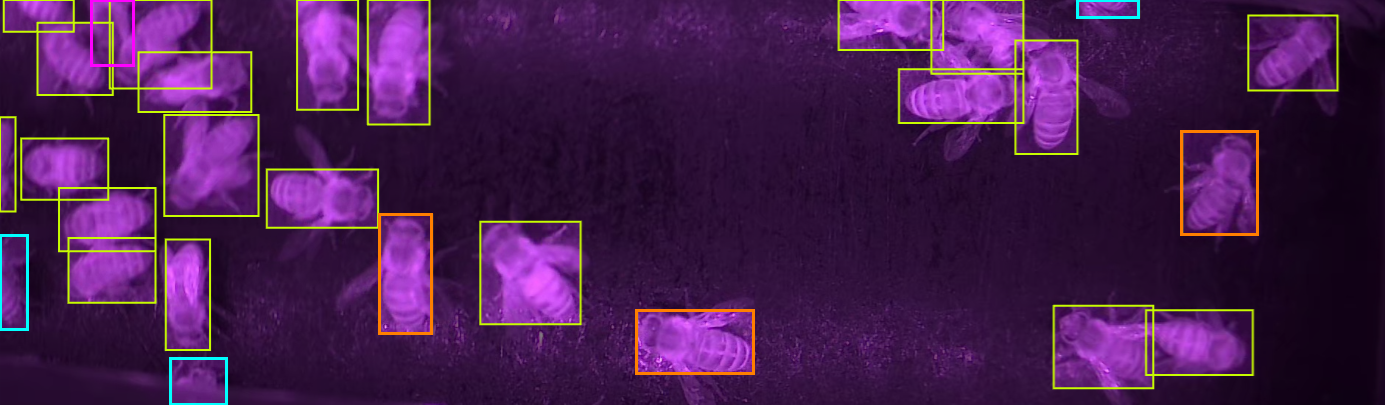
\includegraphics[width = .8\textwidth]{images/annotated_edited.png}
    \caption{Regelkonform annotiertes Bild}
    \label{fig:annotated_edited}
\end{figure}
\noindent
Nachdem alle Bilder mit Bounding Boxes versehen waren, haben wir außerdem die horizontale Spiegelung jeden Bildes zum Datensatz hinzugefügt. Durch diese so genannte \textit{Augmentation} haben wir mit einem geringem Aufwand die Größe des Datensatzes verdoppelt. Die Bounding Boxes haben wir im Darknet-Format exportiert. Dabei wird in einer Textdatei jedes Rechteck durch seine zwei x-Koordinaten und zwei y-Koordinaten gespeichert.\\
Wichtig ist für die Bienenerkennung eine Minimierung der Fehler auf fast null sowie eine sehr geringe Laufzeit, denn in jedem Videoeinzelbild werden alle Pixel untersucht. Deswegen haben wir als Modell zur Objekterkennung das neuronale Netz YOLOv4-tiny gewählt und uns für die YOLO-Implementierung in Darknet, einem Open-Source-Framework für neuronale Netze, entschieden. Es handelt sich dabei um eine verkleinerte Version des neuronalen Netzes YOLOv4. Das ist ein Modell, welches eine sehr hohe Leistungsfähigkeit, also geringe Fehlerzahl aufweist. Seine Besonderheit besteht darin, dass es die Bounding Boxes und die entsprechenden \textit{Scores}, das ist bei uns die Wahrscheinlichkeit, dass in der Box eine Biene ist, in einem Schritt anstatt nacheinander erstellt. Deswegen ist YOLOv4 ein \textit{one-stage detector} und es erhält daher seinen Namen \glqq You Only Look Once - version 4\grqq \, sowie seine hohe Effizienz.\\
YOLOv4-tiny verfügt über nur 29 \textit{convolutional layers} statt 53 und zwei \textit{YOLO layers} statt 3 im YOLOv4 Netzwerk\bibRef{darknet-yolov4}. Deshalb erreicht es eine noch geringere Laufzeit bei Erhaltung hoher Leistungsfähigkeit. Das verringerte auch die Trainingszeit des Modells um den gleichen Faktor. Deswegen konnten wir es auf Google-Colab, einem Cloud-Dienst, der für maximal zwölf Stunden kostenlos leistungsstarke GPU zur Verfügung stellt, vollständig trainieren.\\
\subsection{Implementierung der Videoverfolgung von Bienen}
Für jede Bounding Box von Bienen auf einem Videoeinzelbild wird ein dazugehöriges Bienen-Objekt, das in \textit{bee.py} definiert ist, erstellt. Dann wird nacheinander zu jedem Bienen-Objekt $b_0$ das Bienen-Objekt $b_1$ aus dem letzten Videoeinzelbild ermittelt, sodass der Abstand $d$ der Mittelpunkte von $b_0$ und $b_1$ am kleinsten ist. Wenn $d$ eine Grenze \textit{bee\_dist\_thresh}, die in \textit{settings.py} definiert ist, unterschreitet, nehmen wir an, dass $b_0$ die gleiche Biene wie $b_1$ ist. Deshalb erbt $b_0$ alle Eigenschaften von $b_1$ durch den Aufruf von $b_0.track(b_1)$, insbesondere ob sie infiziert ist. Außerdem löschen wir $b_1$ aus der Liste der Bienen aus dem letzten Videoeinzelbild, um Verdopplungen von Bienen zu verhindern. Wenn $d$ groß ist, dann ist $b_0$ zu keiner Biene aus dem vorherigen Videoeinzelbild nah. Das heißt, $b_0$ ist neu in das Bild gekommen oder hat sich sehr schnell bewegt. Zweiteres ist selten der Fall und führt deshalb zu einem kleinen Fehler.
\subsection{Erstellung eines Modells zur Varroaerkennung}
\subsection{Optimierung der Laufzeit}
Die Laufzeitoptimierung ist bei dem vorliegenden Problem von hoher Relevanz, da das Programm in Echtzeit laufen soll. Technologisch befinden wir uns gerade in der Übergangsphase, sodass Videoanalysen in Echtzeit auf kleinen Geräten schwierig aber möglich sind.\\
Wir haben alle rechenaufwändigen Operationen auf das Python-Modul für Computersicht \textit{cv2} (Computer Vision 2) ausgelagert. Diese behandelt ein Bild als \textit{numpy-array}, denn ein Bild ist eine Tabelle von RGB-Werten. Da \textit{numpy} in C++ implementiert ist, wird das Programm durch diese Auslagerung bis zu $100$ mal schneller. Für die optimale Ausnutzung dessen, haben wir an einen 14-stündigen \textit{cv2}-Kurs auf \url{udemy.com} teilgenommen\bibRef{udemy}.\\
Zur weiteren Verringerung der Laufzeit haben wir zunächst gemessen, welche Operationen einen großen Teil der Laufzeit verursachen. Dafür haben wir eine eigene, nutzerfreundliche \textit{Timer}-Klasse in \textit{timer.py} implementiert und verwendet. Damit haben wir schrittweise mit unserer Methode des Versuchs und Irrtums die Laufzeit weiter verringert.\\
Schon zu Anfang unserer Arbeit haben wir geplant, nur jedes $k$-te Videoeinzelbild zu analysieren. Aus unserem Literaturstudium ist allerdings hervorgegangen, dass alle modernen Videoformate zur Datenkompression die Änderungen zwischen aufeinanderfolgenden Videoeinzelbildern und nicht ganze Bilder speichern. Das ist eine Maßnahme zur so genannten Interframe-Kompression\bibRef{compression}. Für das Programm bedeutet das, dass man deutlich schneller das nächste Videoeinzelbild berechnen kann als zu einem Videoeinzelbild an einer bestimmten Stelle des Videos zu springen.\\
Deshalb haben wir mit unserer \textit{Timer}-Klasse einen eigenen Testaufbau erstellt, mit dem wir verschiedene Laufzeiten berechnen konnten.\\
Wir haben ermittelt, wie sich die Laufzeit $t_{iter}$ pro untersuchtem Bild und die Laufzeit $t_{real}$ pro Videosekunde, in Abhängigkeit von $k$ ändern. Dabei haben wir die Methoden $M1$, bei der man direkt zum $k-1$-nächsten Videoeinzelbild springt und dann das nächste Videoeinzelbild analysiert sowie die Methode $M2$, bei der man mehrfach das nächste Videoeinzelbild aufruft und bei jedem $k$-ten Aufruf das Bild analysiert, verglichen.
Dafür haben wir auf dem gleichen Gerät diese Werte ermittelt:
\begin{figure}[htb!]
    \centering
    \begin{tabular}{p{.07\linewidth}|p{.07\linewidth}|p{.5\linewidth}}
        Name & Wert & Definition \\ \hline
        $t_j$ & $44,7 \ms$ & Zeit zum Springen zu einem Videoeinzelbild \\ \hline
        $t_s$ & $5,4 \ms$ & Zeit zum Springen zum nächsten Videoeinzelbild \\ \hline
        $t_a$ & $29,2 \ms$ & Zeit zum Einlesen und Analysieren des nächsten Videoeinzelbilds
    \end{tabular}
\end{figure}\\
Für die Methoden $M1$ und $M2$ kann man die Laufzeiten so berechnen:
\begin{figure}[htb!]
    \centering
    \begin{tabular}{p{.07\linewidth}|p{.2\linewidth}|p{.2\linewidth}|p{.2\linewidth}|p{.2\linewidth}}
        $n$ & $t_{iter, M1}(k)$ & $t_{real, M1}(k)$ & $t_{iter, M2}(k)$ & $t_{real, M2}(k)$\\ \hline
        $1$ & $t_a + t_j$ & $(t_a + t_j) \cdot 30$ & $t_a$ & $t_a \cdot 30$\\
        $2$ & $t_a + t_j$ & $(t_a + t_j) \cdot 30 / 2$ & $t_a + t_s$ & $(t_a+t_s) \cdot 30 / 2$\\
        $3$ & $t_a + t_j$ & $(t_a + t_j) \cdot 30 / 3$ & $t_a + 2t_s$ & $(t_a+2t_s) \cdot 30 / 3$\\
        $\vdots$ & $\vdots$ & $\vdots$ & $\vdots$ & $\vdots$\\
        $x$ & $t_a + t_j$ & $(t_a + t_j) \cdot 30 / x$ & $t_a + (x-1)t_s$ & $(t_a+(x-1)t_s) \cdot 30 / x$
    \end{tabular}
\end{figure}\\
Damit können wir Graphen für die Laufzeiten der Algorithmen erstellen.
\begin{figure}[H]
    \centering
    \begin{minipage}{.45\textwidth}
        \begin{tikzpicture}[scale = .8]
            \begin{axis}[
                ymin = 0,
                ymax = 2.75,
                axis lines = left,
                xlabel = \(x\),
                ylabel = {$t_{real}(x) / \mathrm{s}$},
            ]
            \addplot [
                domain=1:12,
                samples=100, 
                color=blue,
                ]
                {0.03*(29.2 + 44.7)/x};
            \addlegendentry{$t_{real, M1}(x)$}
            \addplot [
                domain=1:12, 
                samples=100, 
                color=red,
            ]
            {0.03*(29.2 + 5.4*(x-1))/x};
            \addlegendentry{$t_{real, M2}(x)$}
            \end{axis}
        \end{tikzpicture}
        \caption{$M1-M2$-Vergleich}
        \label{fig:m1-m2}
    \end{minipage}
    \begin{minipage}{.45\textwidth}
        \begin{tikzpicture}[scale = .8]
            \begin{axis}[
                ymin = 0,
                ymax = 1.1,
                axis lines = left,
                xlabel = \(x\),
                ylabel = {$t_{real}(x) / \mathrm{s}$},
            ]
            \addplot [
                domain=1:5, 
                samples=100, 
                color=red,
            ]
            {0.03*(29.2 + 5.4*(x-1))/x};
            \addlegendentry{$t_{real, M2}(x)$}
            
            \end{axis}
        \end{tikzpicture}
        \caption{$M2$-Bewertung}
        \label{fig:m2}
    \end{minipage}
\end{figure}
\noindent
$k > 5$ würde zu einer zu geringen zeitlichen Auflösung führen, um die Erkennung aller Milben zu gewährleisten. Weil Abbildung \autoref{fig:m1-m2} zeigt, dass die Methode $M2$ für kleine $k$ deutlich schneller ist, haben wir uns deshalb für die Implementierung der Methode $M2$ entschieden.\\
Aus Abbildung \autoref{fig:m2} geht darüber hinaus hervor, dass ab $k = 3$ eine weitere Erhöhung von $k$ zu keiner starken Senkung der Laufzeit von $M2$ führt, weshalb $k \in \{1, 2, 3\}$ eine sinnvolle Wahl ist. Unter diesen drei Werten kann $k$ je nach Rechenleistung des Computers angepasst werden.

% ---------------------------------------
% -----------Milbenbekämpfung------------       1 - 2 Seiten ~ Albert, Daniel
% ---------------------------------------
\newpage
\section{Umsetzung der Milbenbekämpfung}
\subsection{Ideen zum Aufbau}

\subsection{Durchführung erster Versuche mit Lasern}

% \subsection{Darstellung der Ergebnisse auf einer Website} -> nehmen wir nur ausführlich, falls wir noch Platz füllen müssen



% ---------------------------------------
% ------Fortsetzungsmöglichkeiten--------       1 - 2 Seiten ~ Albert
% ---------------------------------------
\newpage
\section{Fortsetzungsmöglichkeiten}


% ---------------------------------------
% -------------Auswertung----------------           1 Seite ~ Alle
% ---------------------------------------
\newpage
\section{Zusammenfassung}

% ---------------------------------------
% ---------------Anhang------------------
% ---------------------------------------
\newpage
\section{Anhang}

\subsection{Zu Kapitel \autoref{section:Theory}}
\begin{figure}[H]
    \centering
    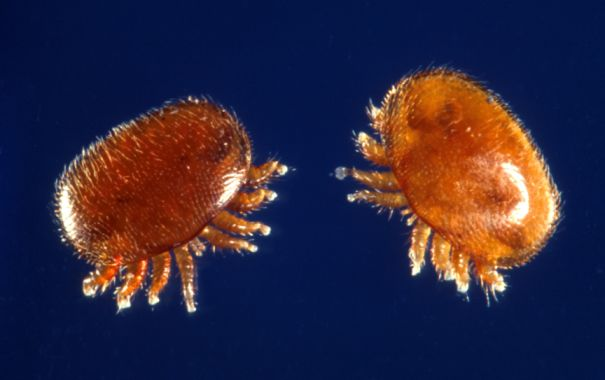
\includegraphics[width = .7\textwidth]{images/Varroamilbe.jpg}
    \caption{Weibliche Varroa destructor}
    \label{fig:annotated_edited}
\end{figure}

\begin{figure}[H]
    \centering
    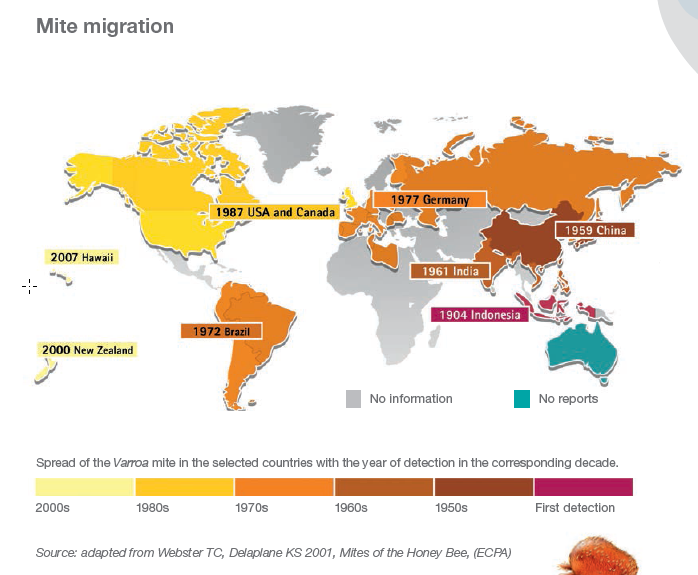
\includegraphics[width = .7\textwidth]{images/Verbreitung Varroamilbe.png}
    \caption{Ausbreitung der Milbe Varroa destructor}
    \label{fig:annotated_edited}
\end{figure}

\subsection{Zu Kapitel \autoref{section:Vorbetrachtungen}}
\begin{figure}[H] \label{fig:technical-sketch}
    \centering
    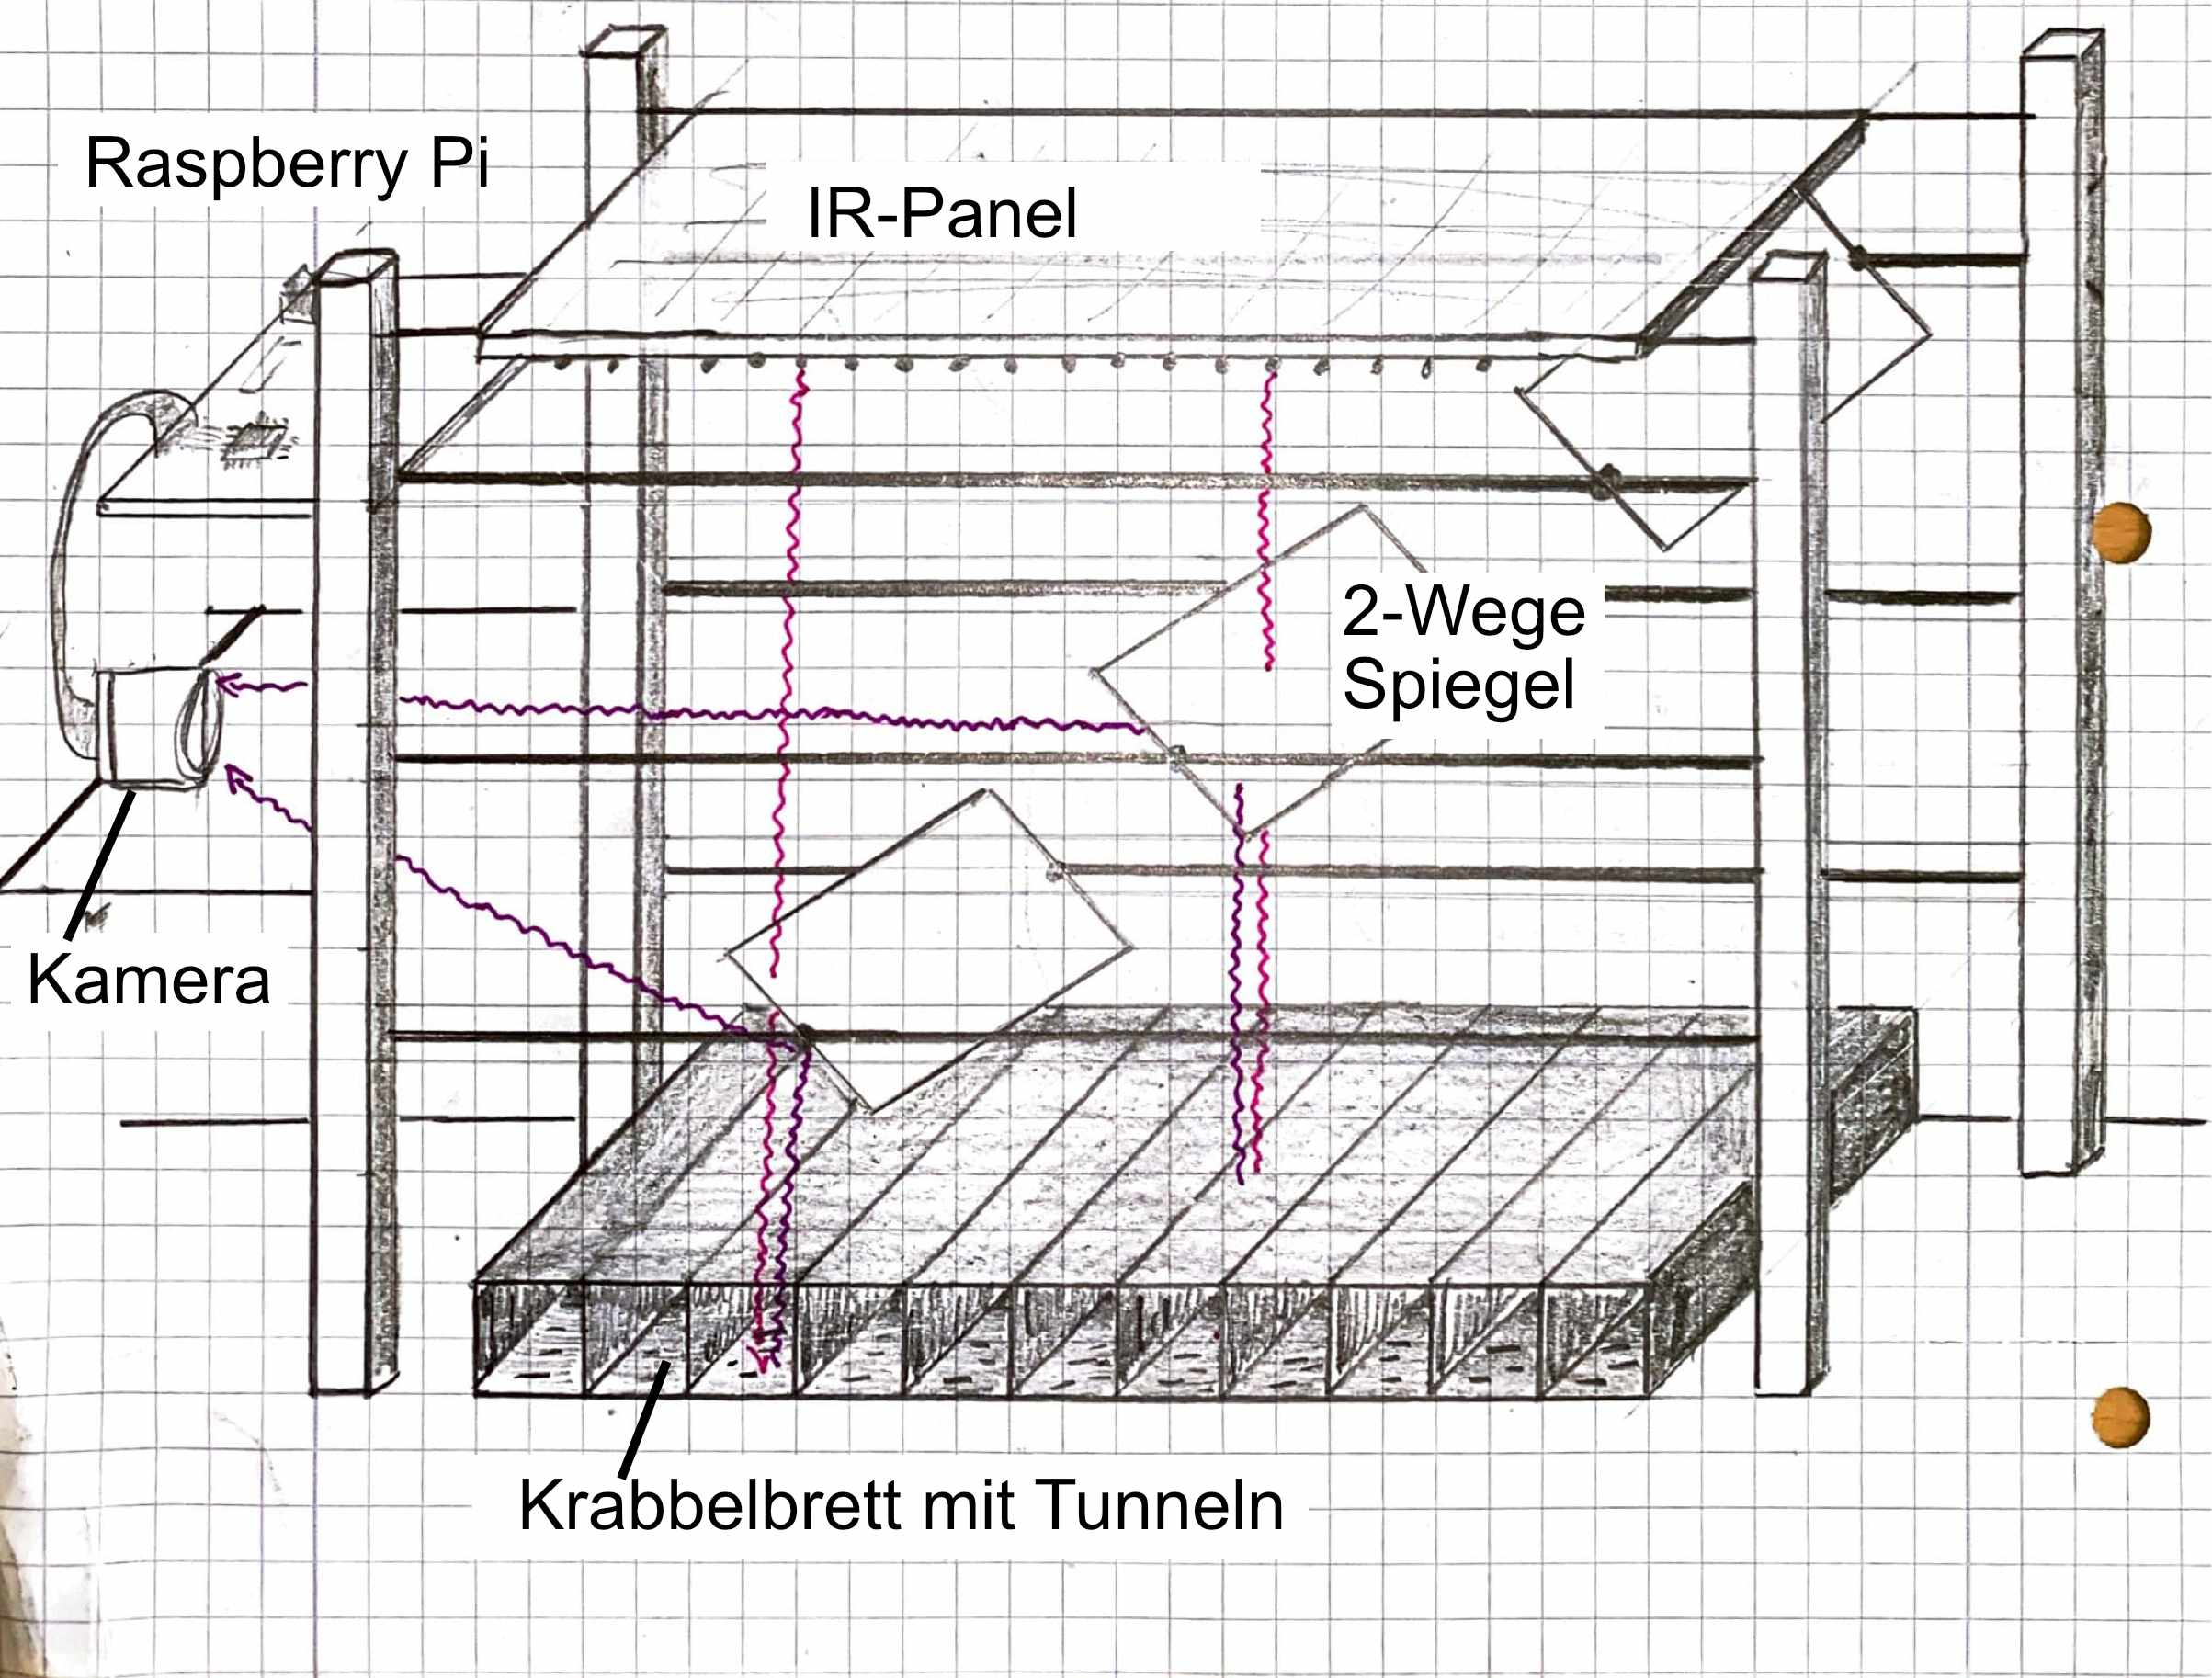
\includegraphics[width=.9\textwidth]{images/technische Skizze 1.jpg}
    \caption{Technische Skizze einer mechanischen Vorrichtung, die durch Spiegel immer eine Biene fokussiert\\
    \textit{Quelle: Eigenarchiv}}
\end{figure}

\begin{figure}[H] \label{fig:mechanics-test}
    \centering
    \begin{subfigure}{.49\textwidth}
        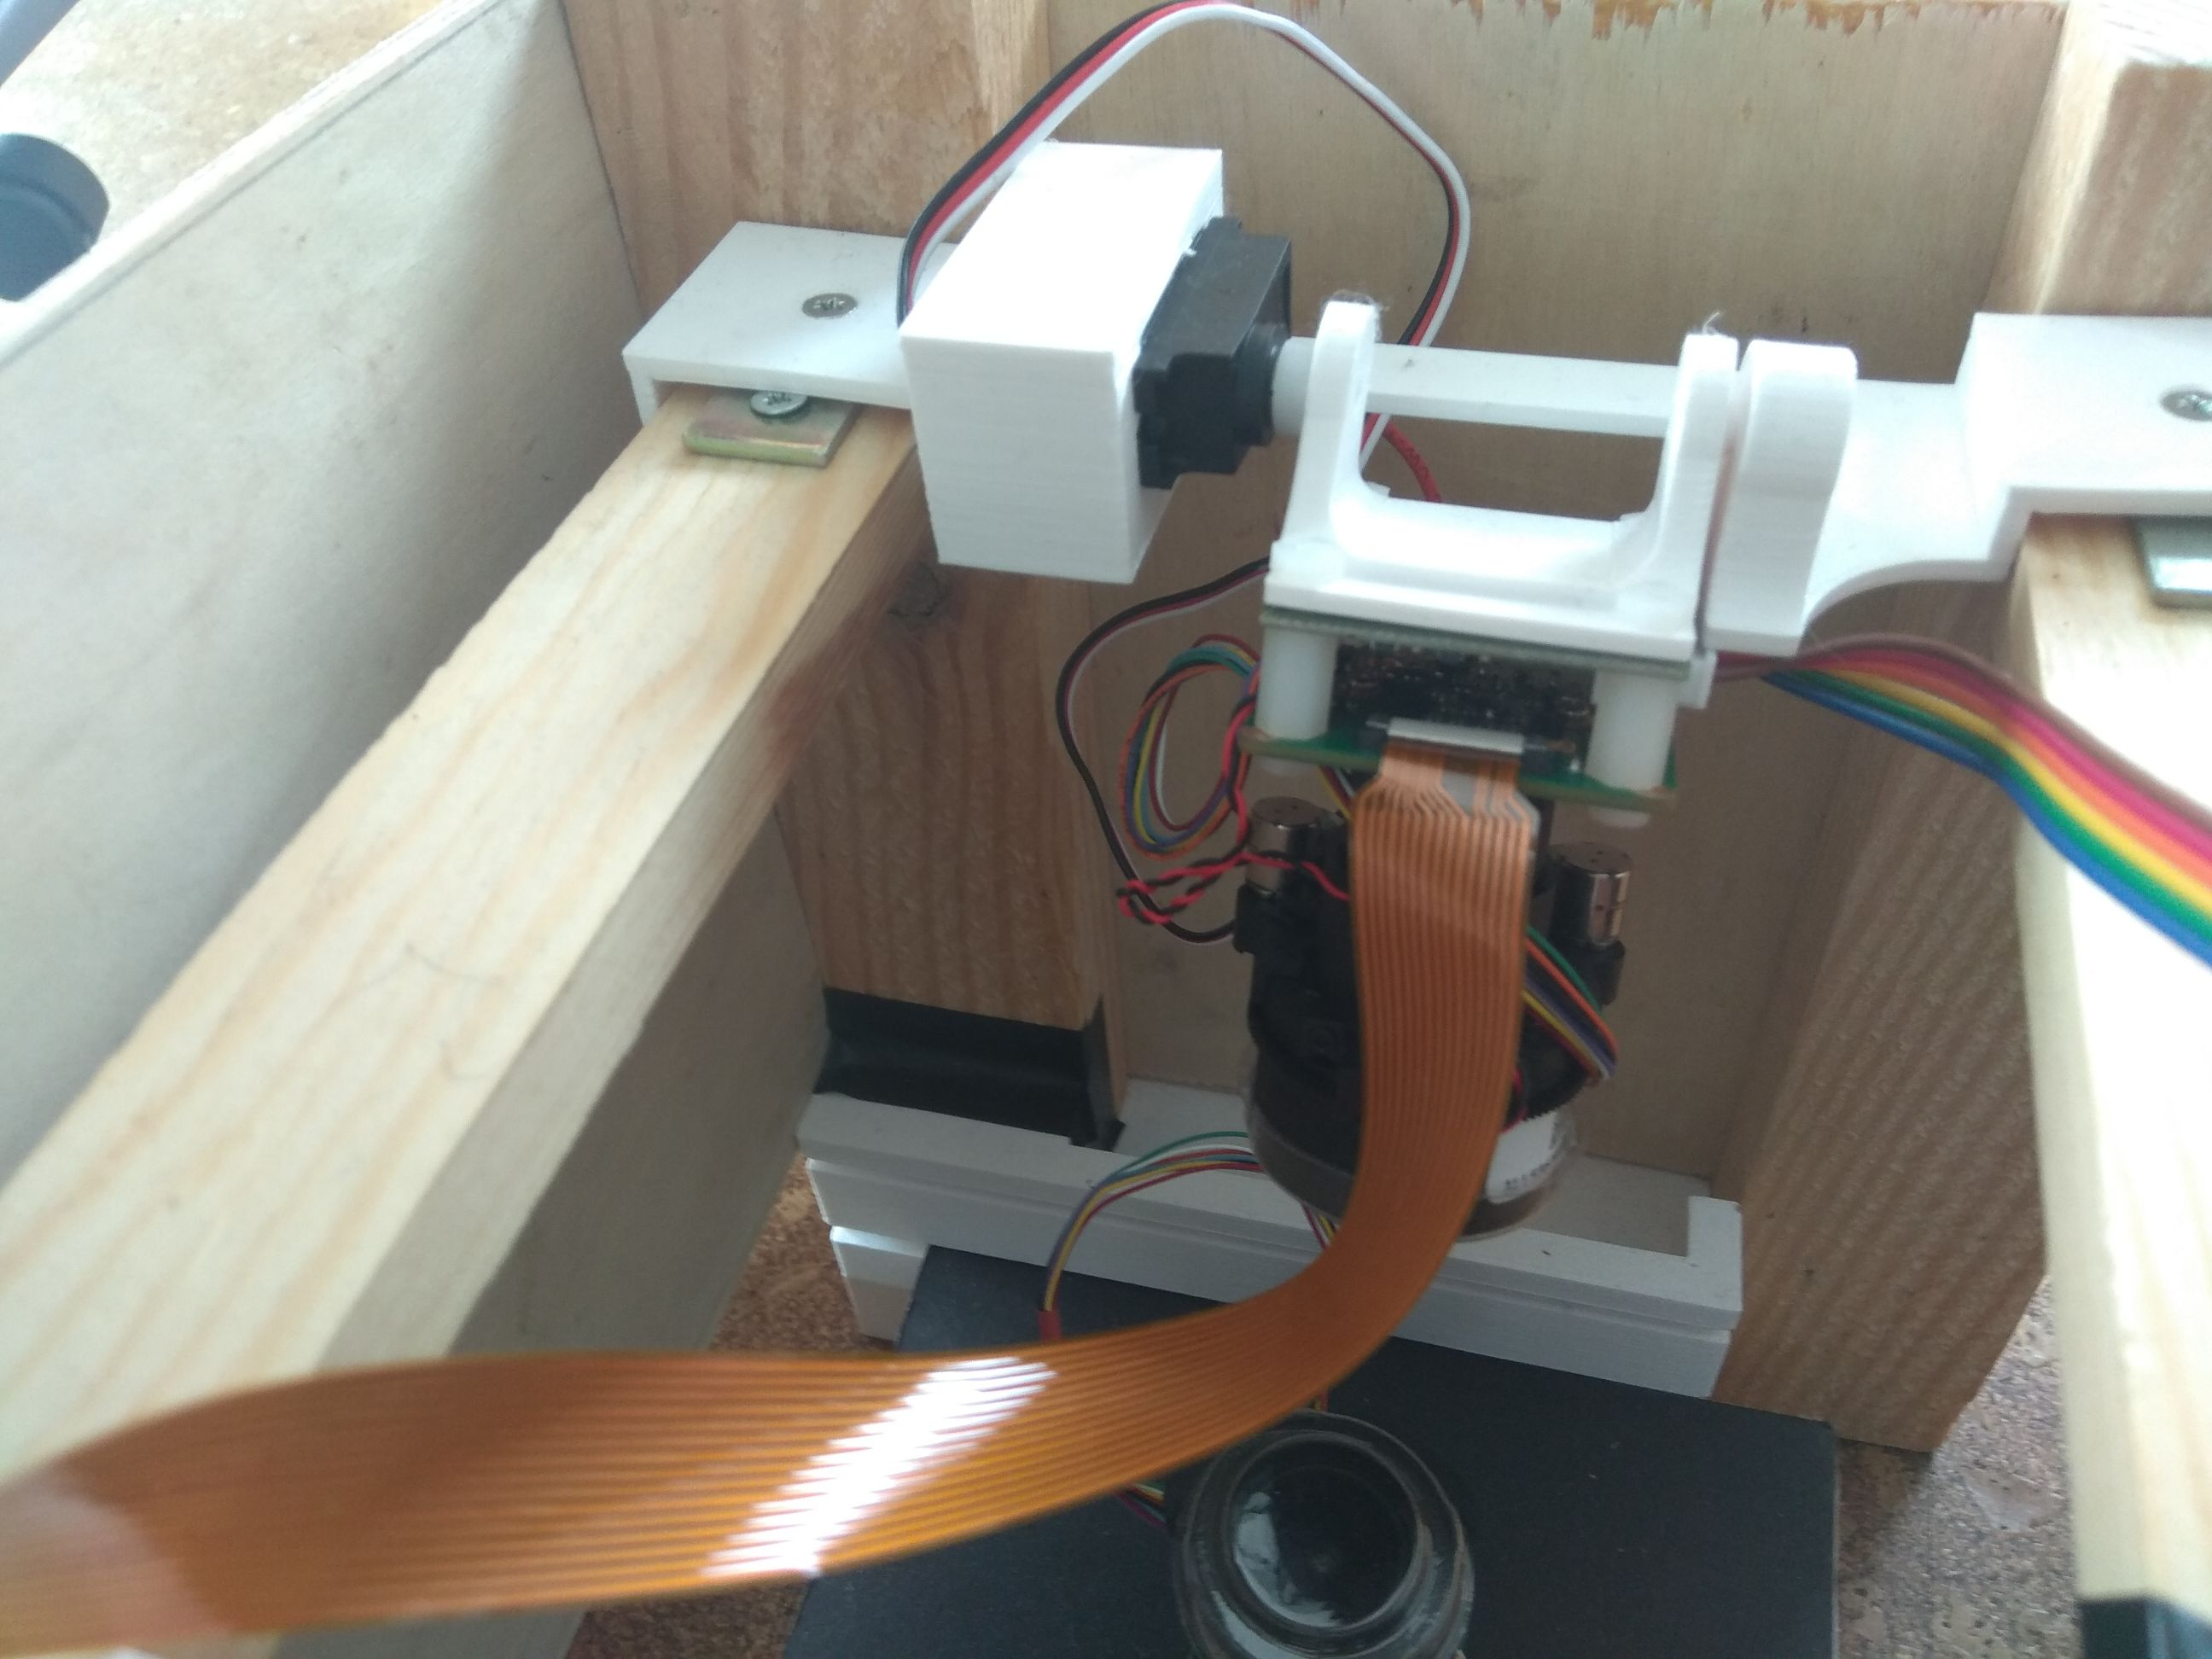
\includegraphics[height=.2\textheight]{images/mechanics_test_1.jpg}
    \end{subfigure}
    \begin{subfigure}{.49\textwidth}
        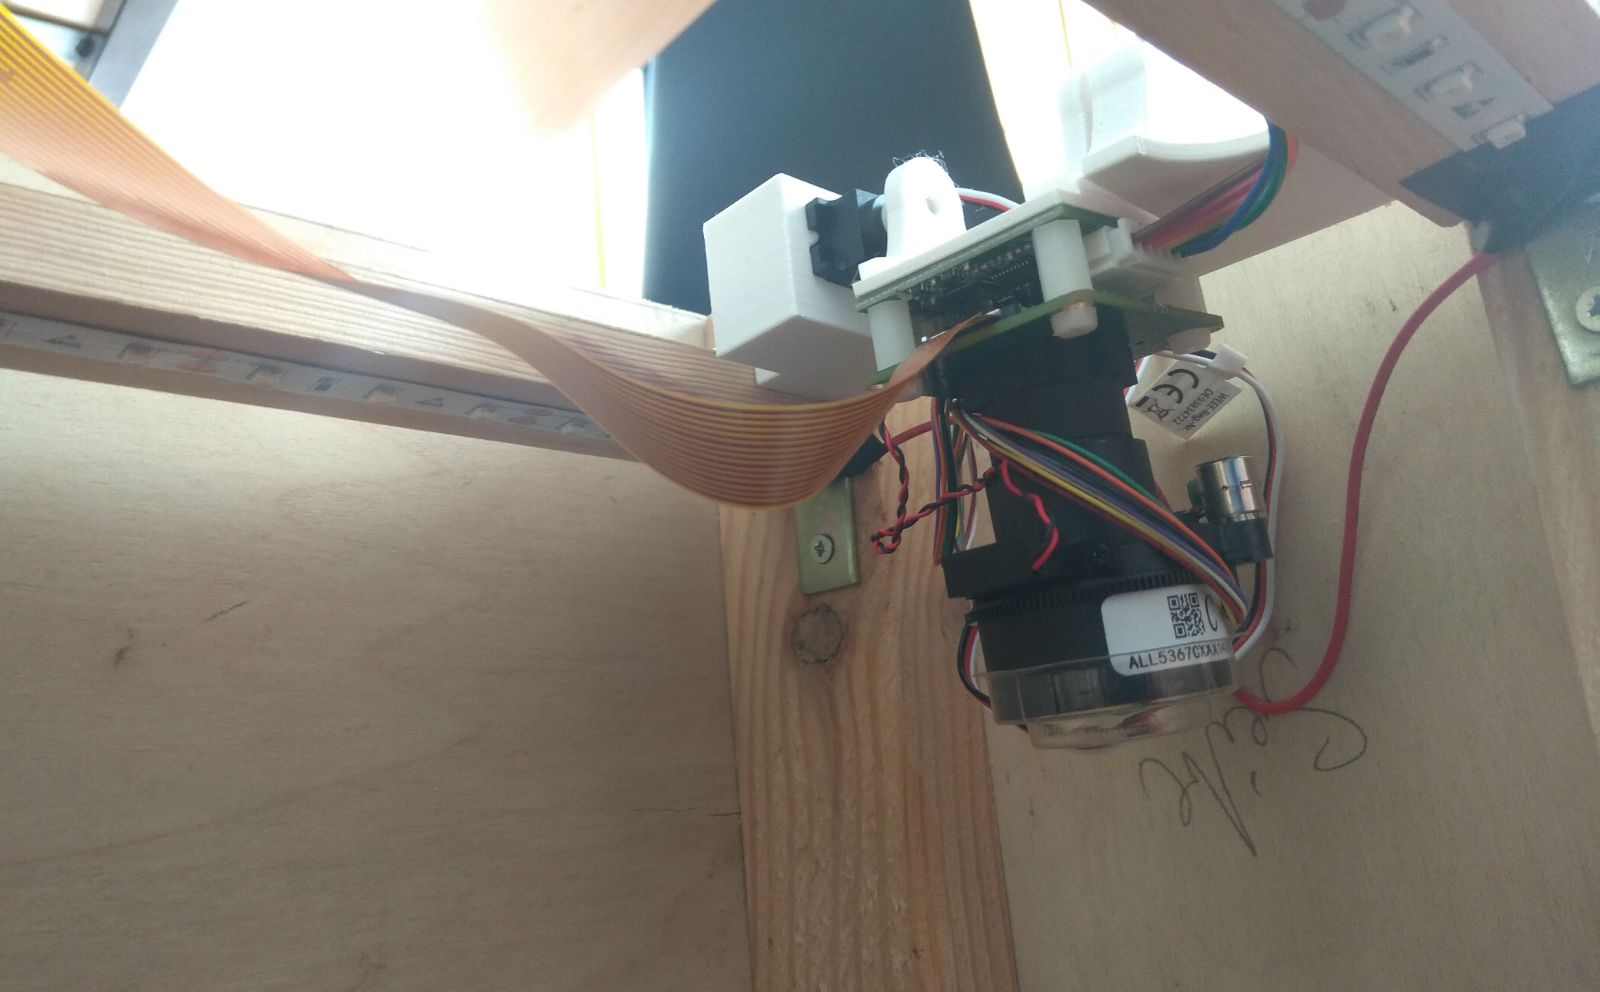
\includegraphics[height=.2\textheight]{images/mechanics_test_2.jpg}
    \end{subfigure}
    \caption{Versuchsaufbau zum Testen eines mechanischen Lösungsansatzes: Der Servo kann die Kamera schwenken \\
    \textit{Quelle: Eigenarchiv}}
\end{figure}

\begin{figure}[H]\label{fig:moving-cameras-considerations}
    \centering
    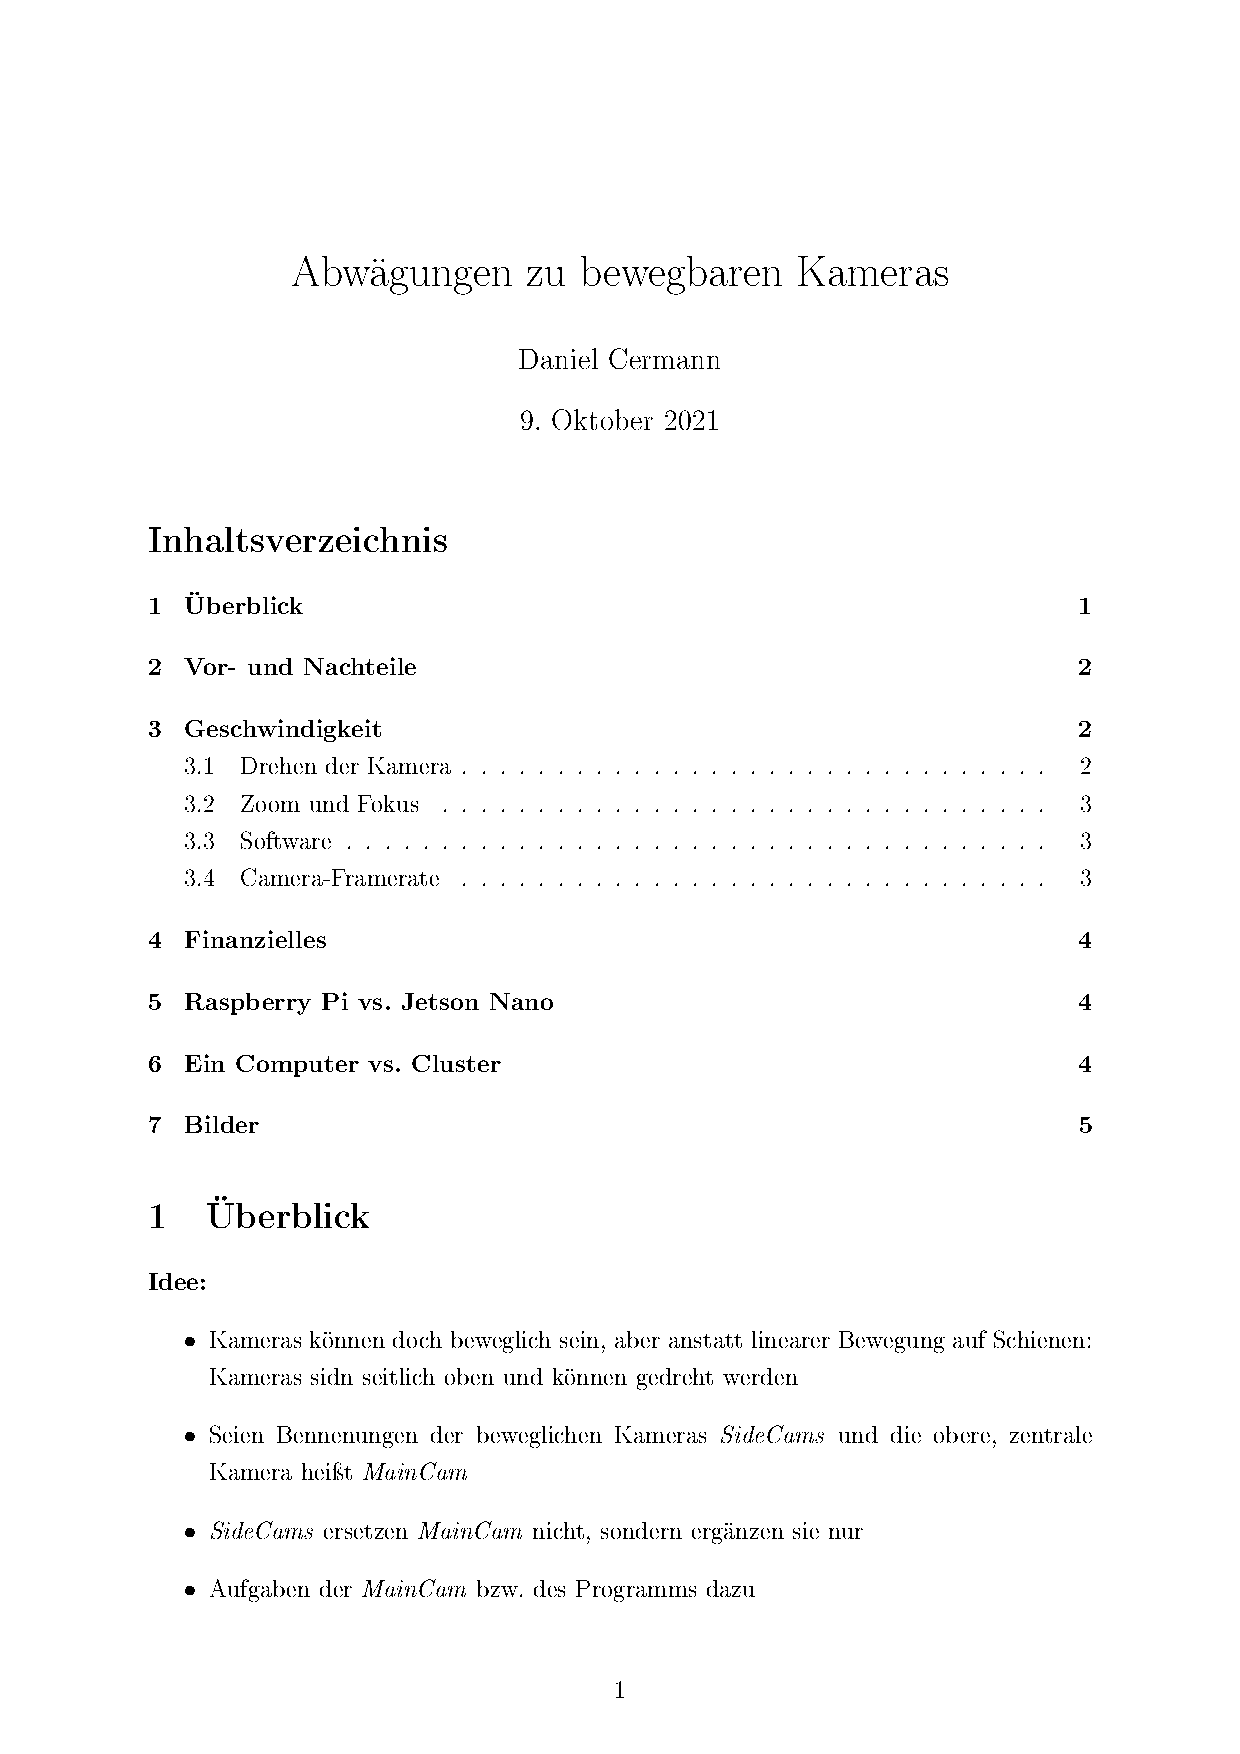
\includegraphics[page=1, scale=.3]{images/TPZ_Cameras_Idea.pdf}
    \includegraphics[page=2, scale=.3]{images/TPZ_Cameras_Idea.pdf}    
    \includegraphics[page=3, scale=.3]{images/TPZ_Cameras_Idea.pdf}    
    \includegraphics[page=4, scale=.3]{images/TPZ_Cameras_Idea.pdf}    
    \caption{Unsere Abwägungen zu bewegbaren Kameras \\
    \textit{Quelle: Eigenarchiv}}
\end{figure}

\begin{figure}[H] \label{fig:bee-vision}
    \centering
    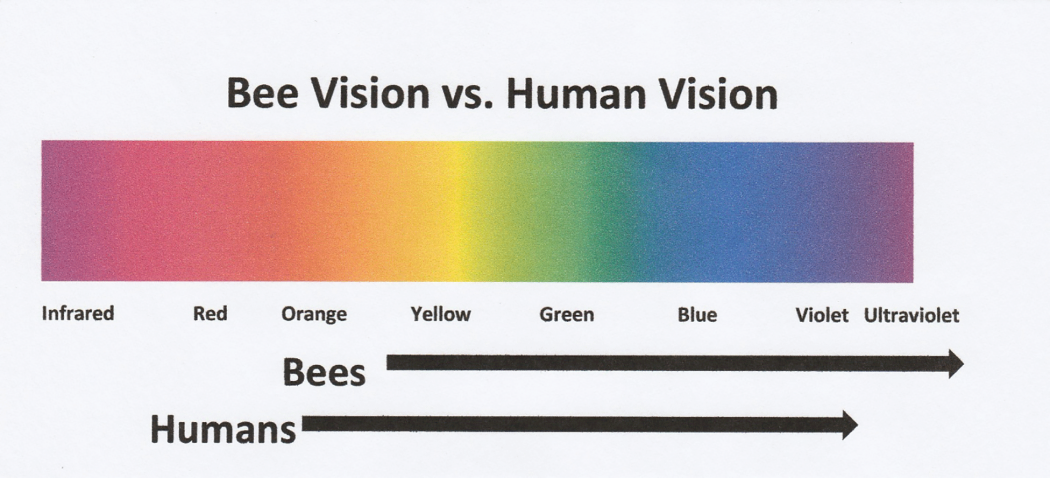
\includegraphics[width=.9\textwidth]{images/bee_vision.png}
    \caption{Der von Bienen sichtbare Bereich des Lichtspektrums \\
    \textit{Quelle: \url{https://www.beeculture.com/bees-see-matters/}}}
\end{figure}

\subsection{Zu Kapitel \autoref{section:Prototypen}}
\begin{figure}[H] \label{fig:power-supply-complete}
    \centering
    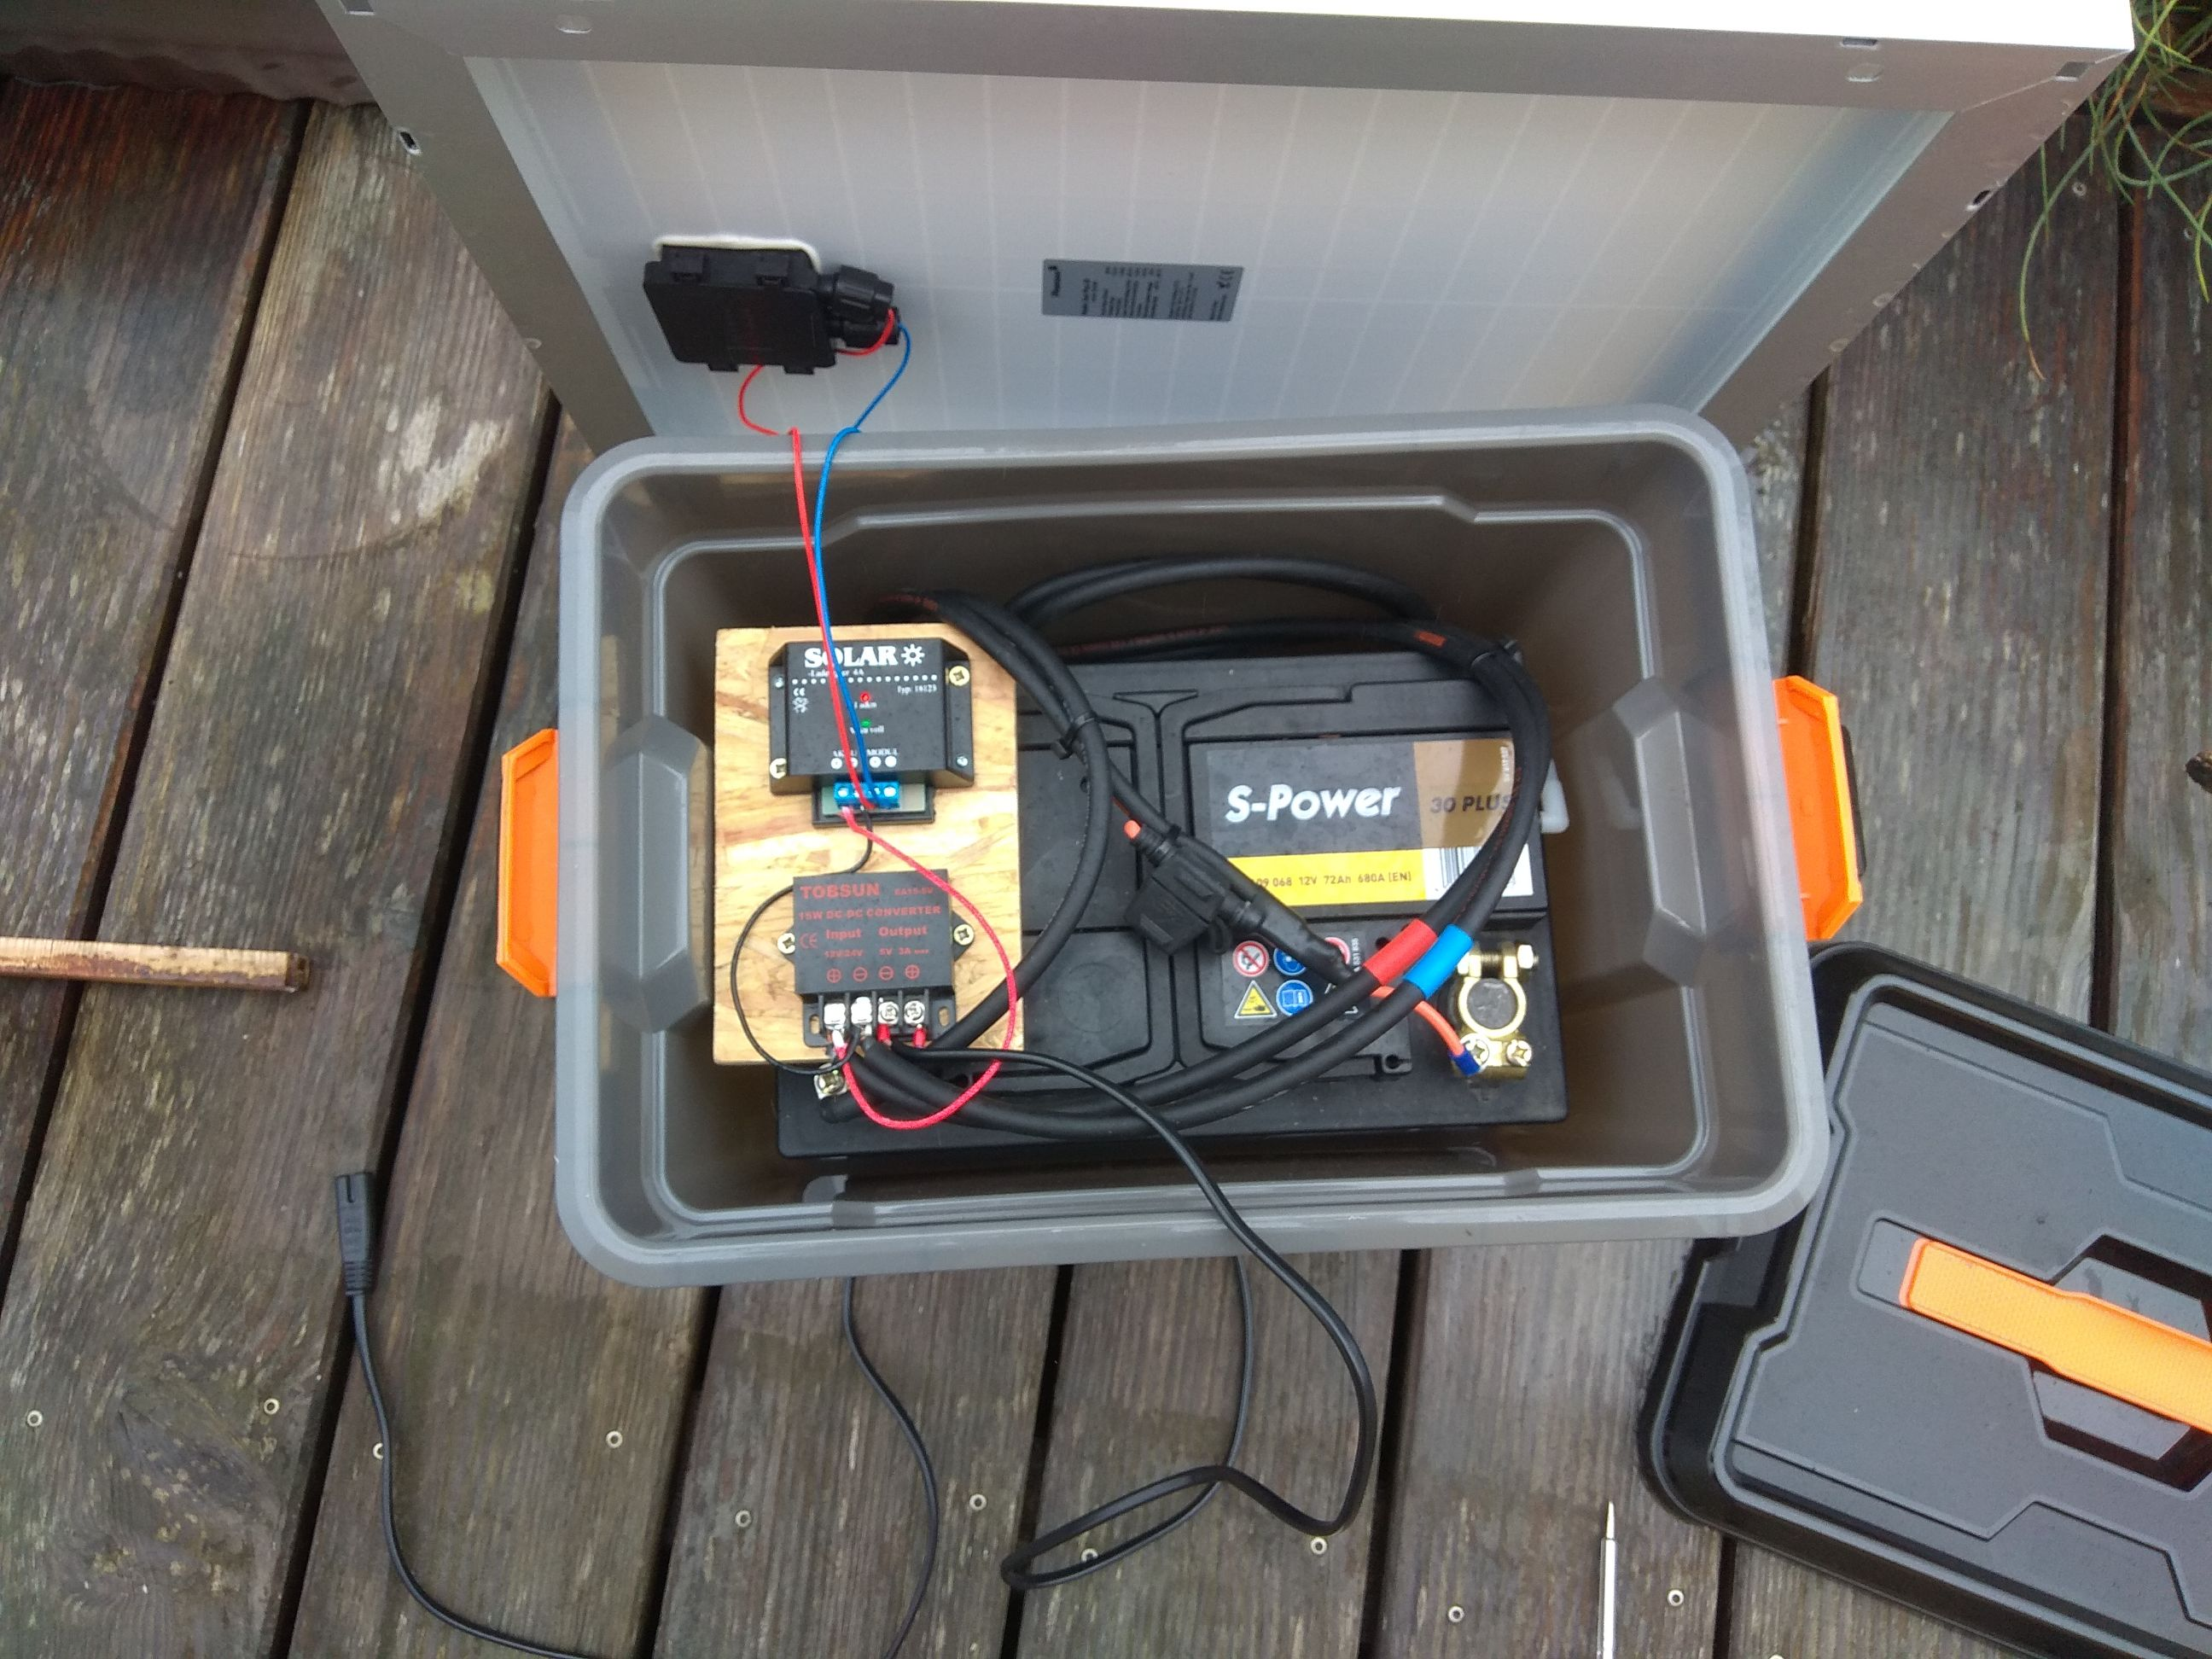
\includegraphics[width=.9\textwidth]{images/power_supply.jpg}
    \caption{Die Stromversorgung für unsere Prototypen \\
    \textit{Quelle: Eigenarchiv}}
\end{figure}

\begin{figure}[H] \label{fig:first-generation-1}
    \centering
    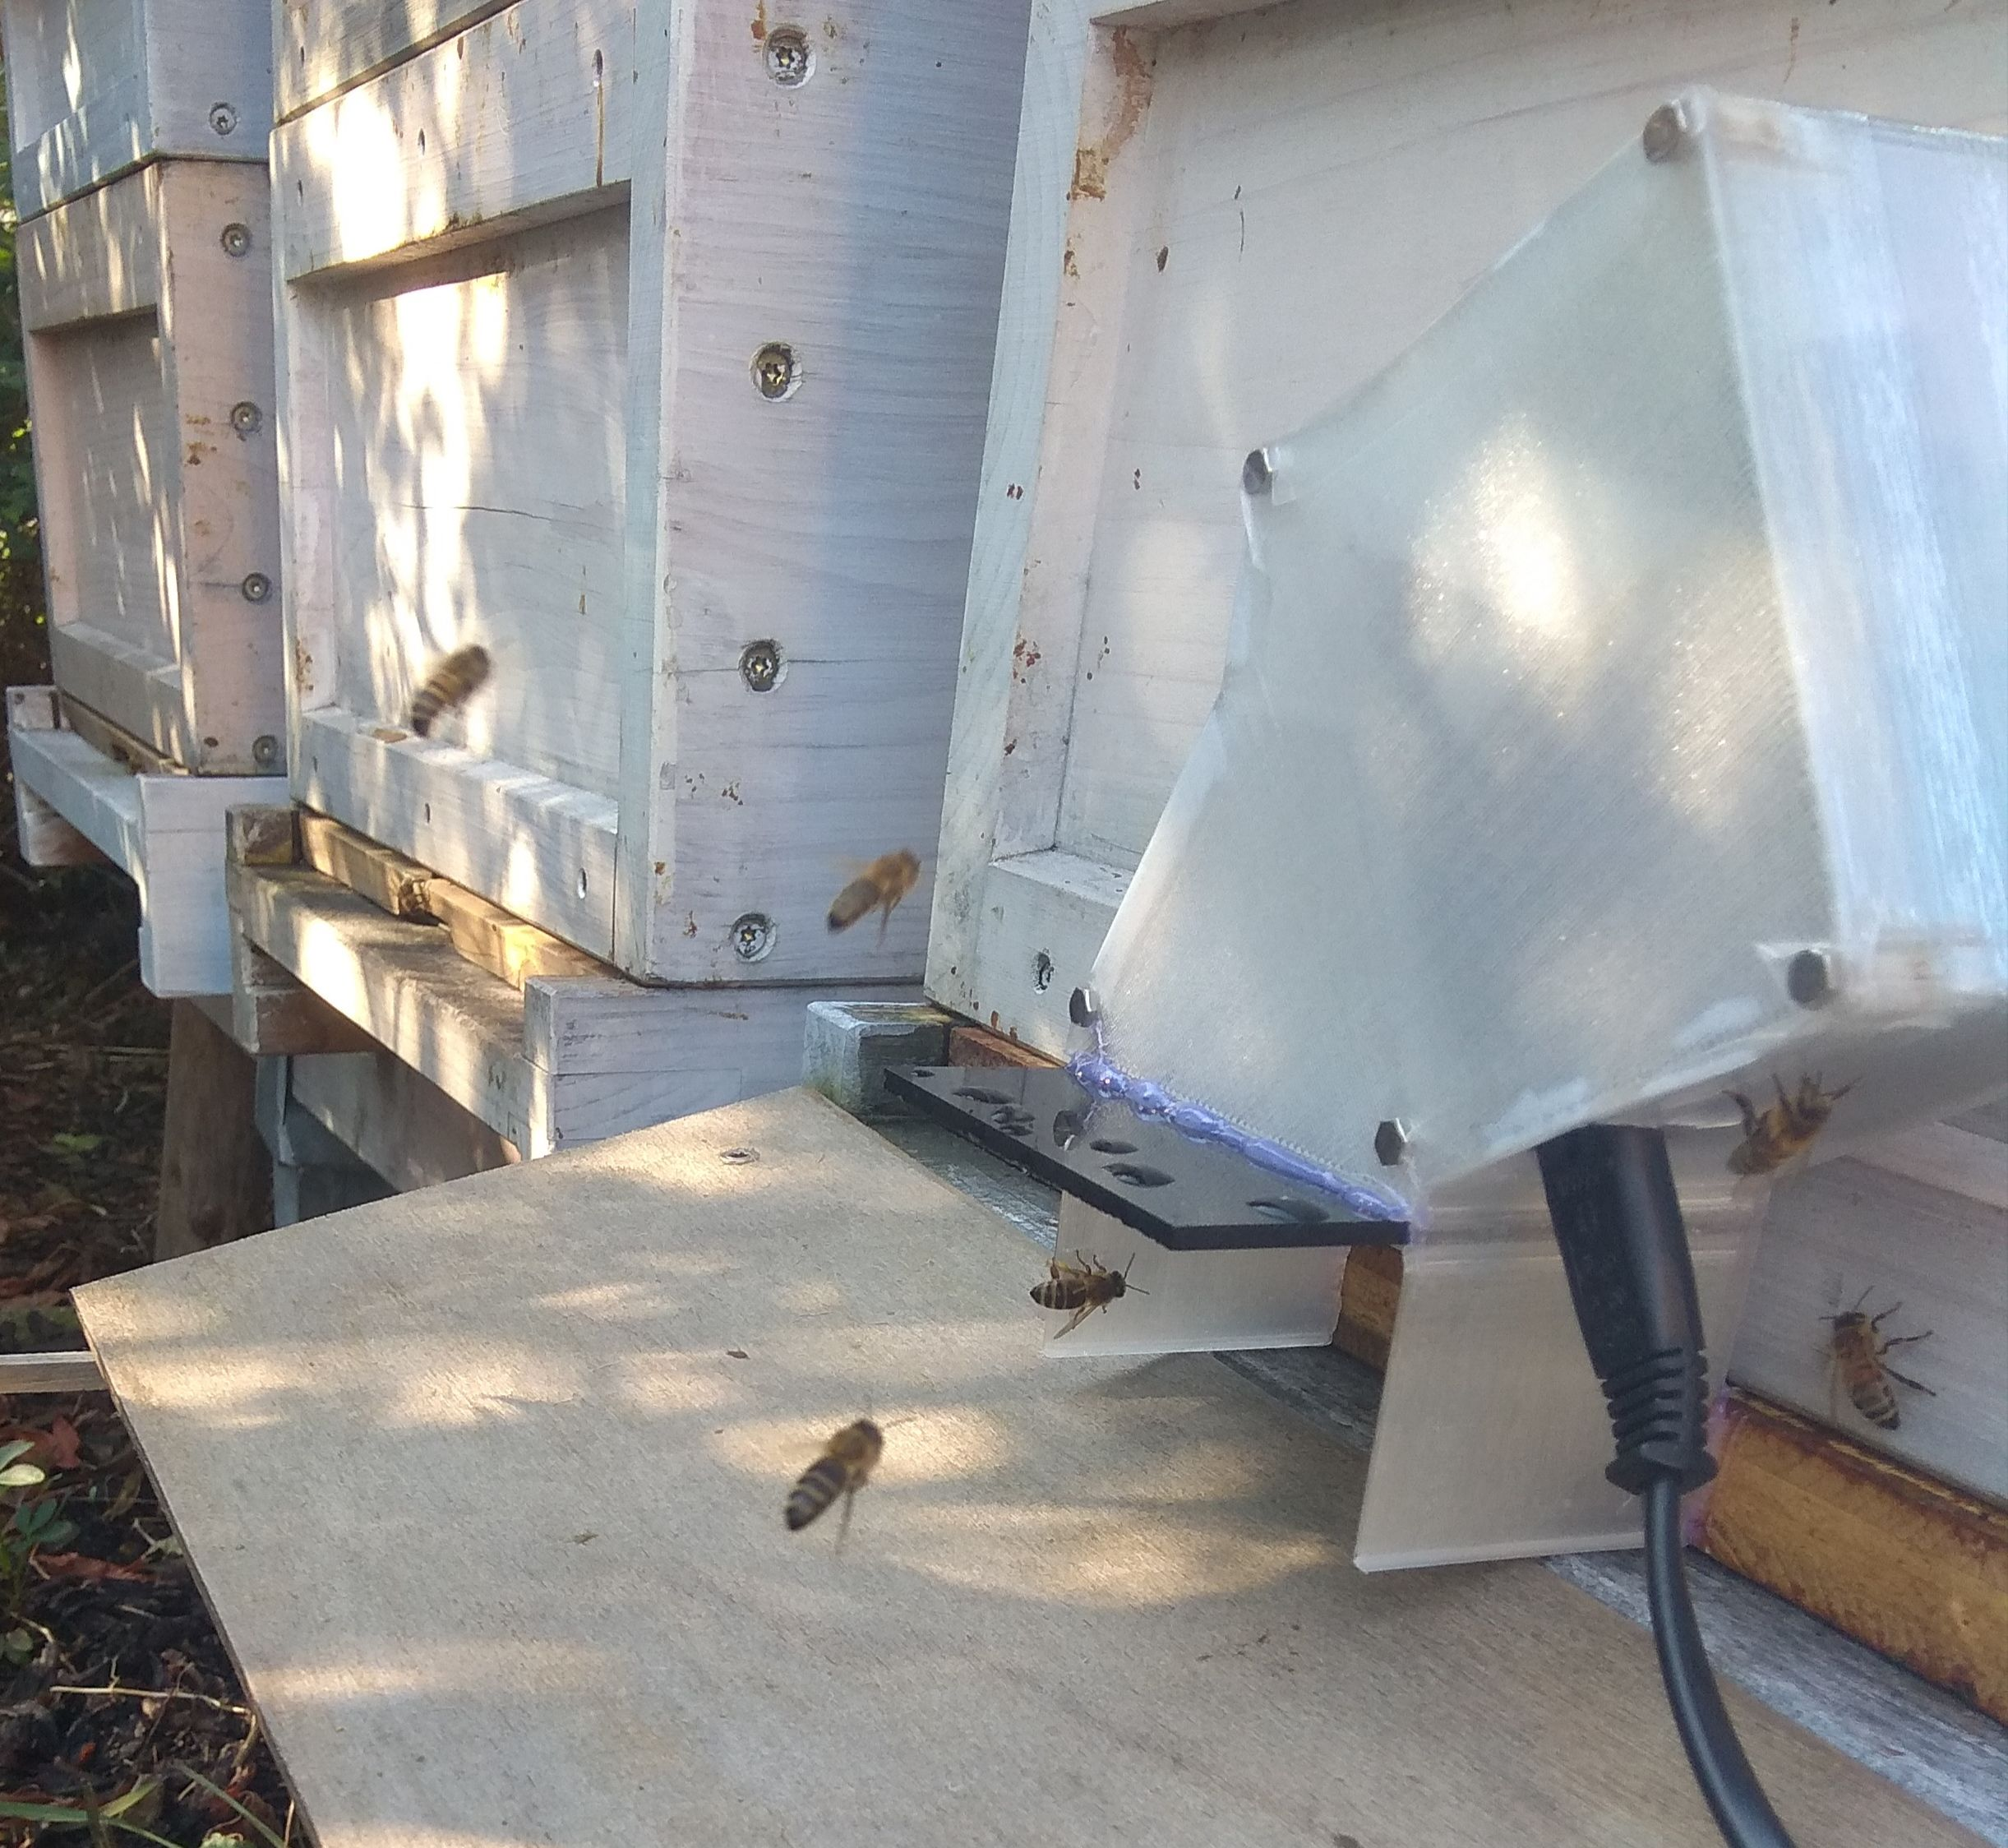
\includegraphics[width=.8\textwidth]{images/first_prototype_on_hive.jpg}
    \caption{Erster Prototyp über beim Überwachen des verkleinerten Fluglochs \\
    \textit{Quelle: Eigenarchiv}}
\end{figure}
\begin{figure}[H] \label{fig:first-generation-2}
    \centering
    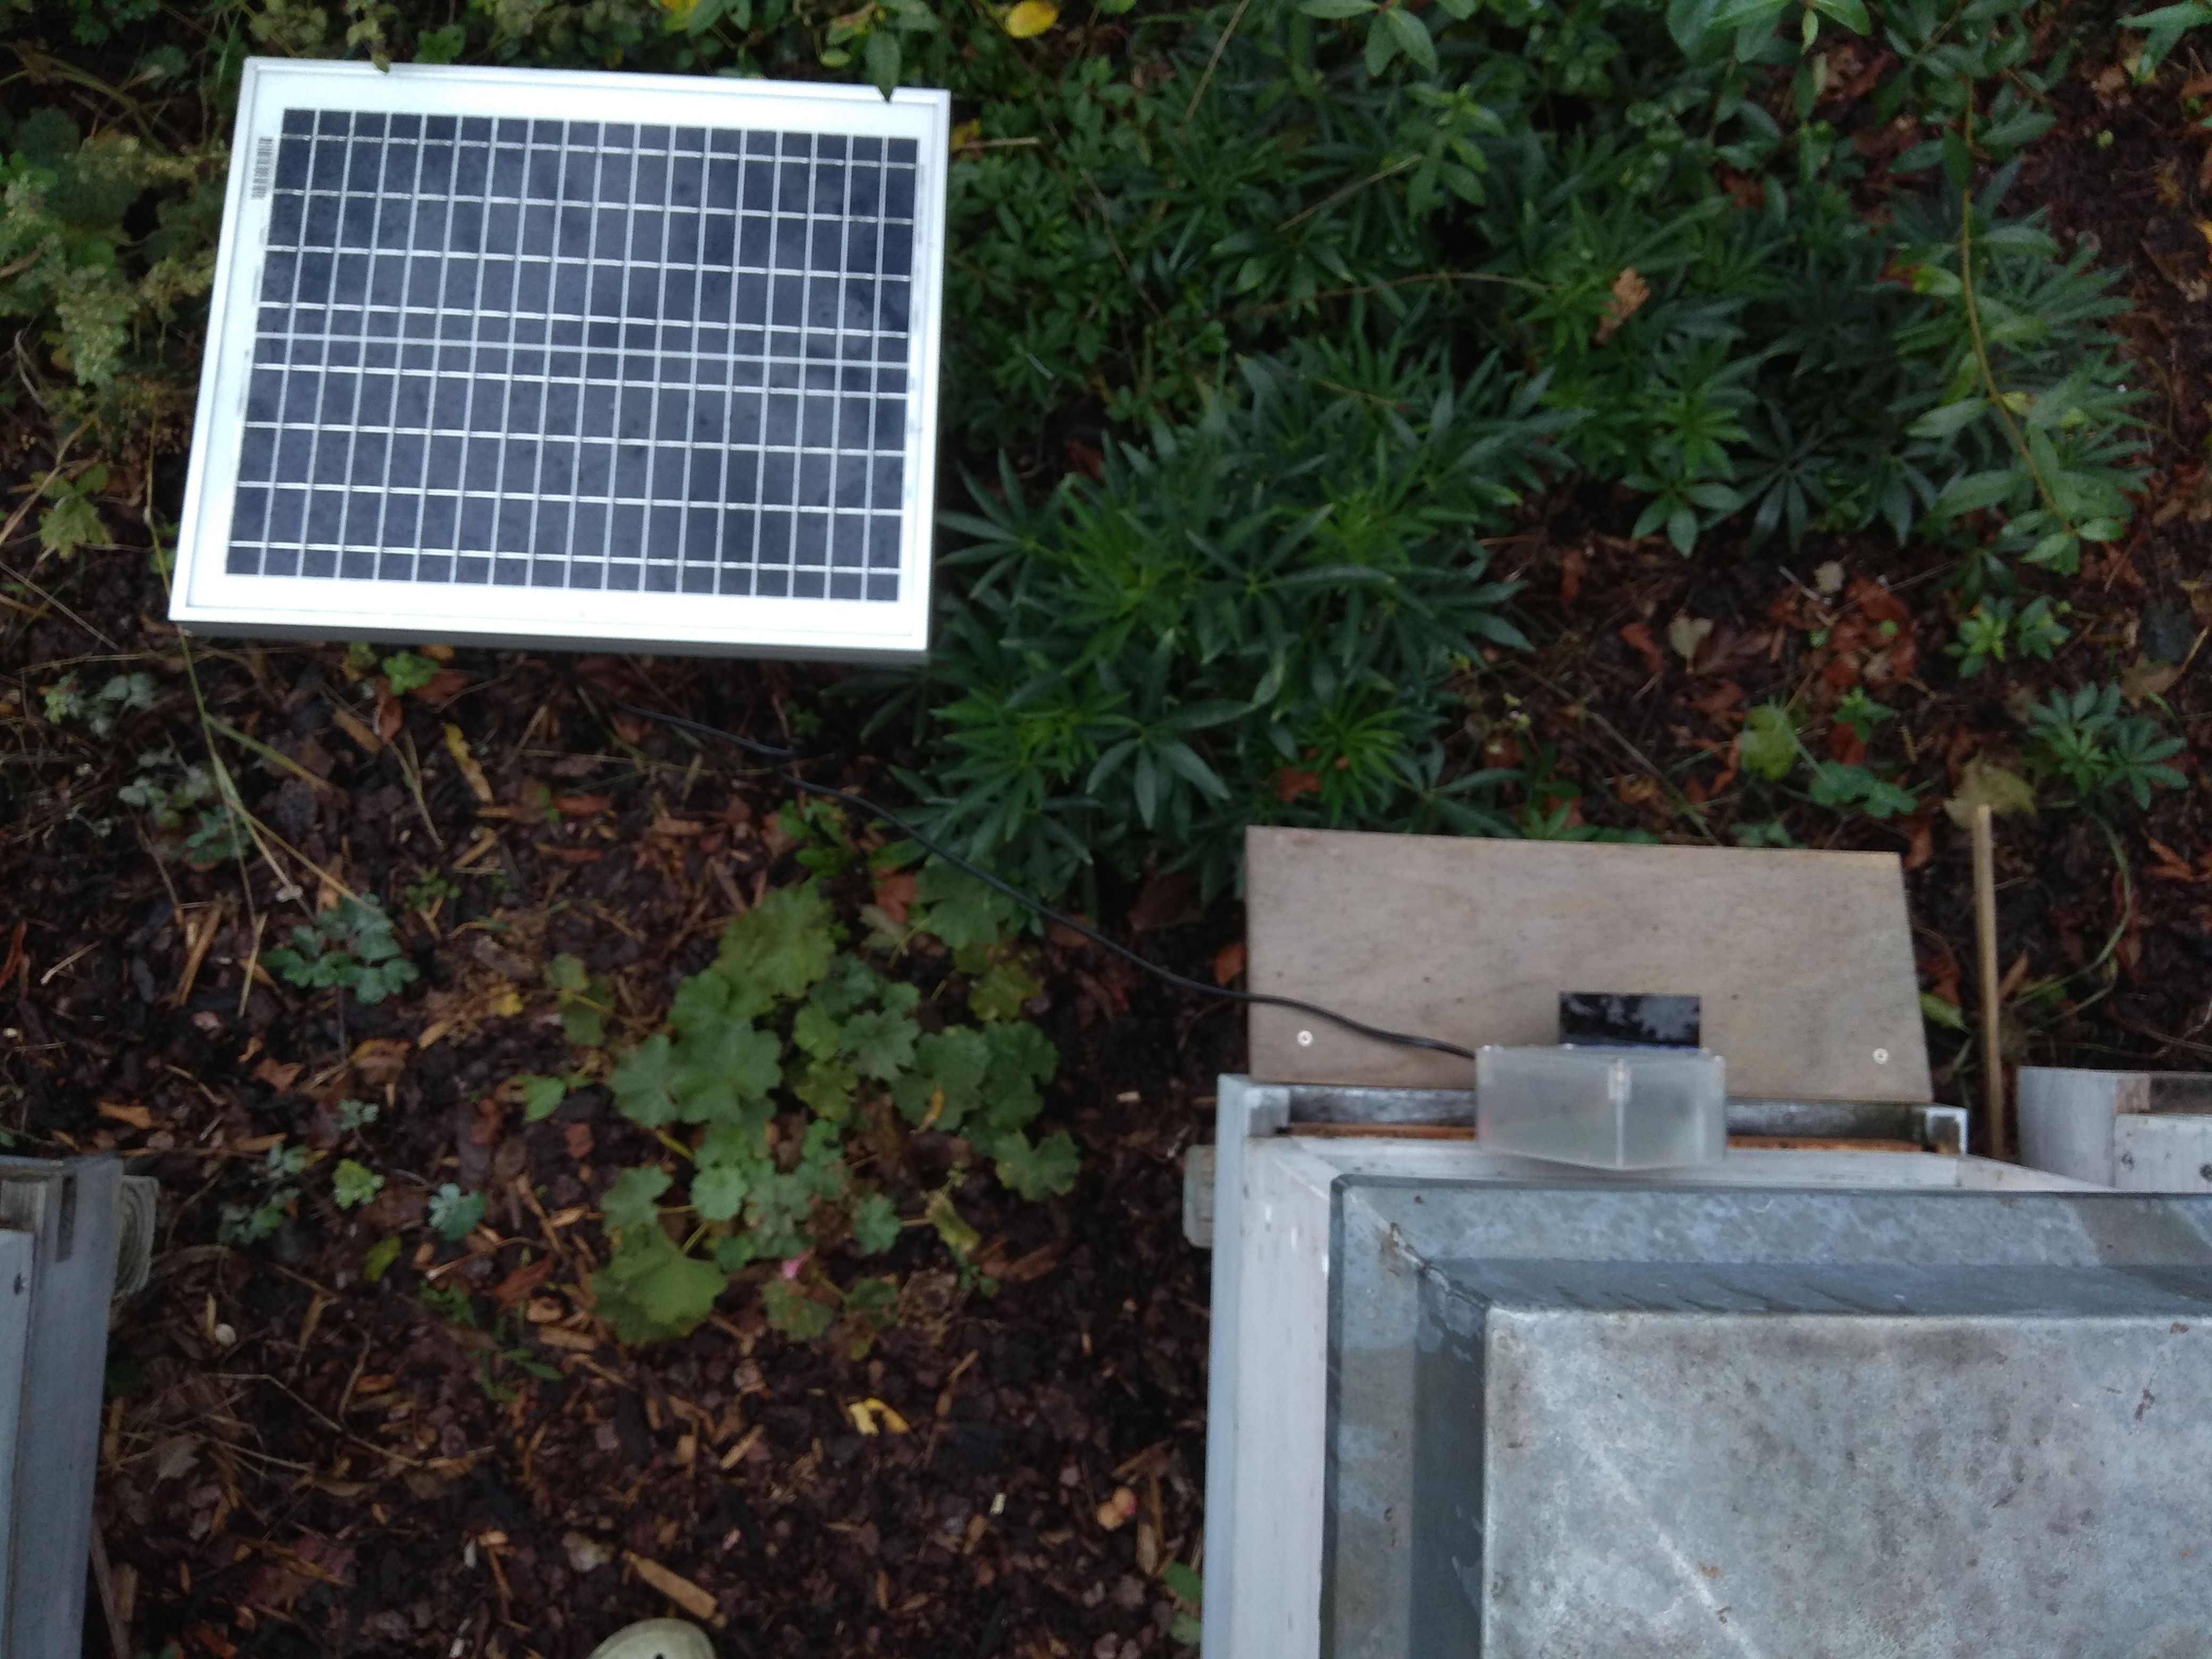
\includegraphics[width=.8\textwidth]{images/first_prototype_birds_eye_view.jpg}
    \caption{Gesamtaufbau des ersten Versuchs \\
    \textit{Quelle: Eigenarchiv}}
\end{figure}
\begin{figure}[H] \label{fig:first-generation-3}
    \centering
    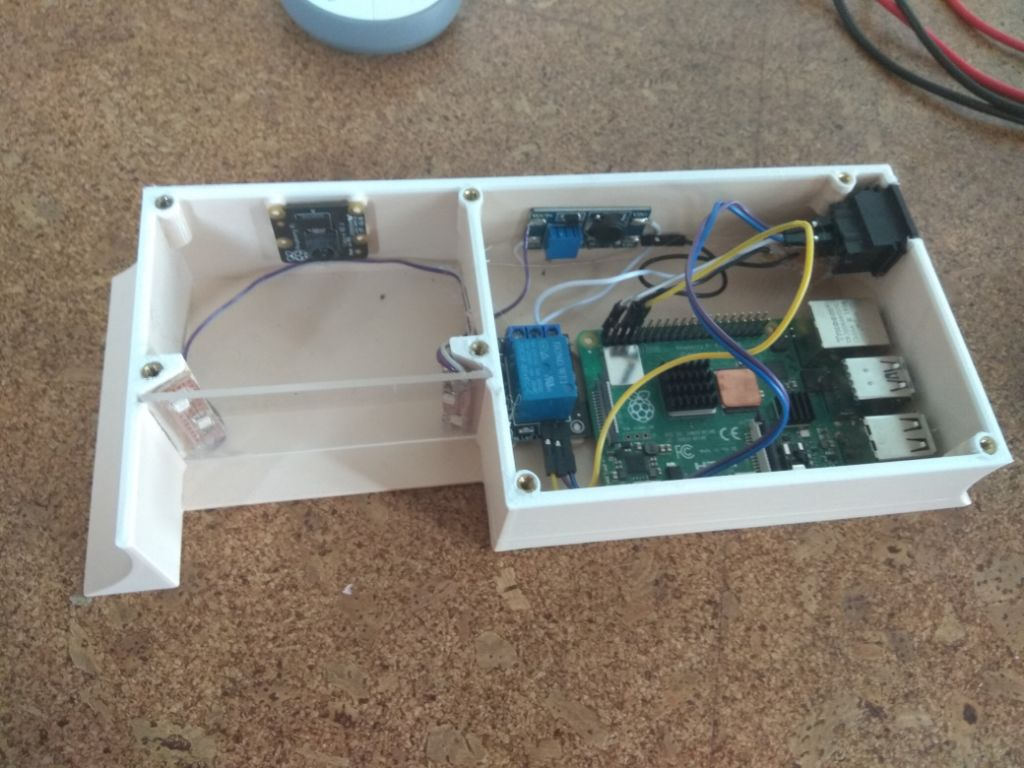
\includegraphics[width=.8\textwidth]{images/second_prototype.jpg}
    \caption{Technischer Aufbau einer verbesserten Version des ersten Tests \\
    \textit{Quelle: Eigenarchiv}}
\end{figure}

\begin{figure}[H] \label{fig:first-generation-result}
    \centering
    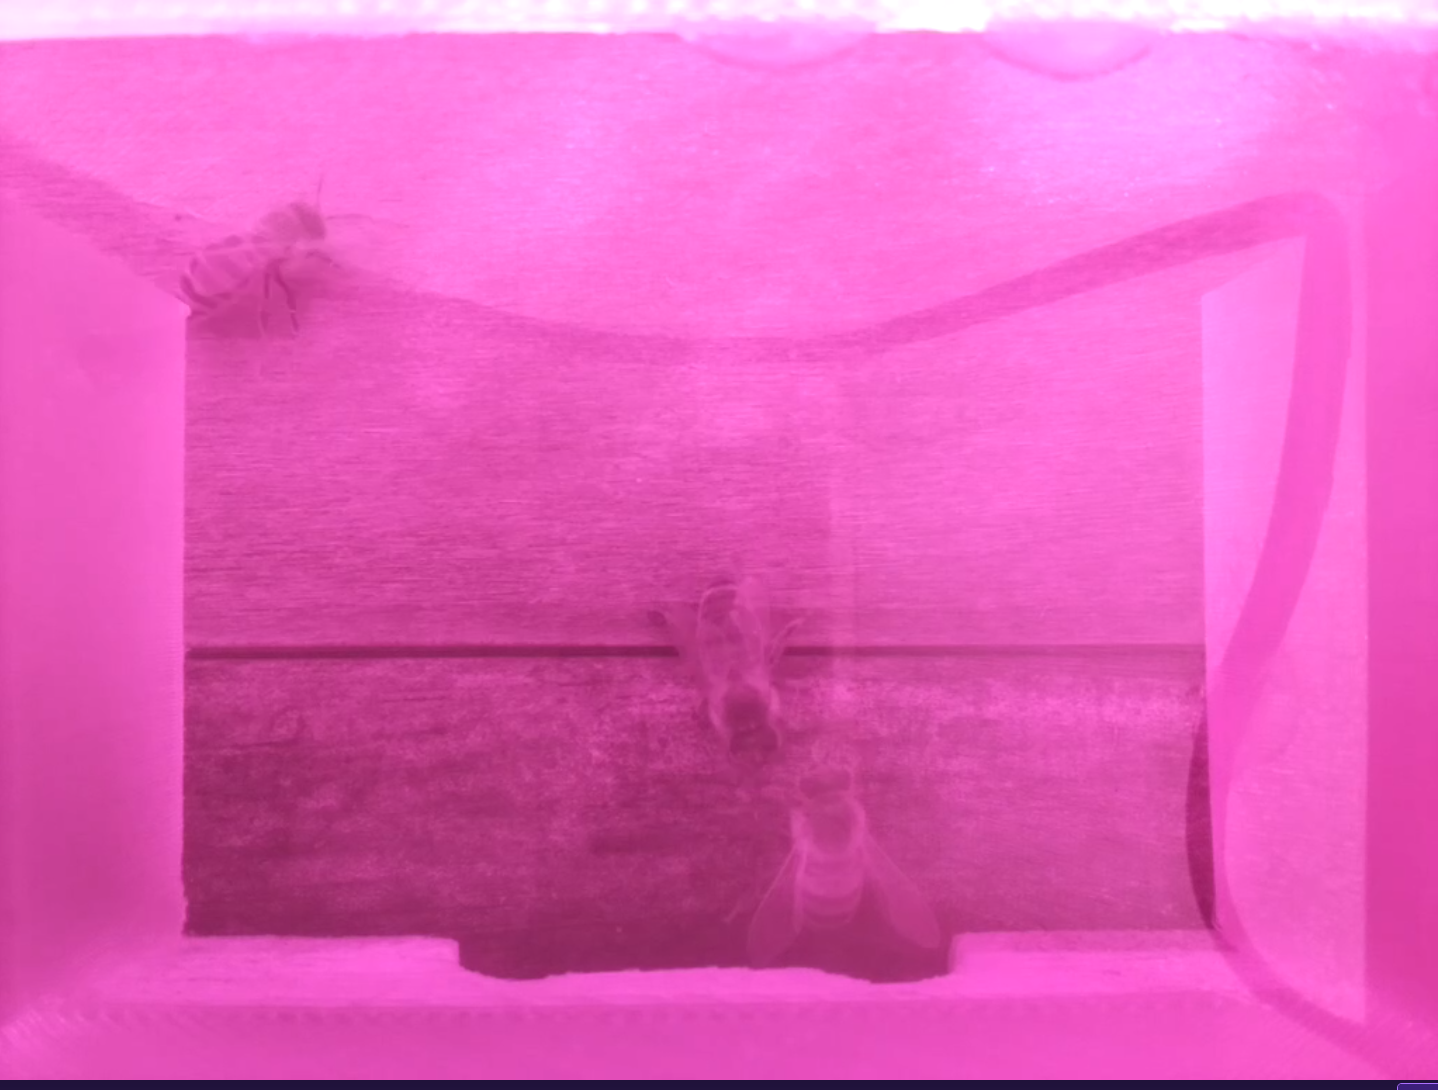
\includegraphics[width=.8\textwidth]{images/results_first_prototype.png}
    \caption{Vom ersten Prototypen aufgenommes Bild\\
    \textit{Quelle: Eigenarchiv}}
\end{figure}

\begin{figure}[H] \label{fig:second-generation-production}
    \centering
    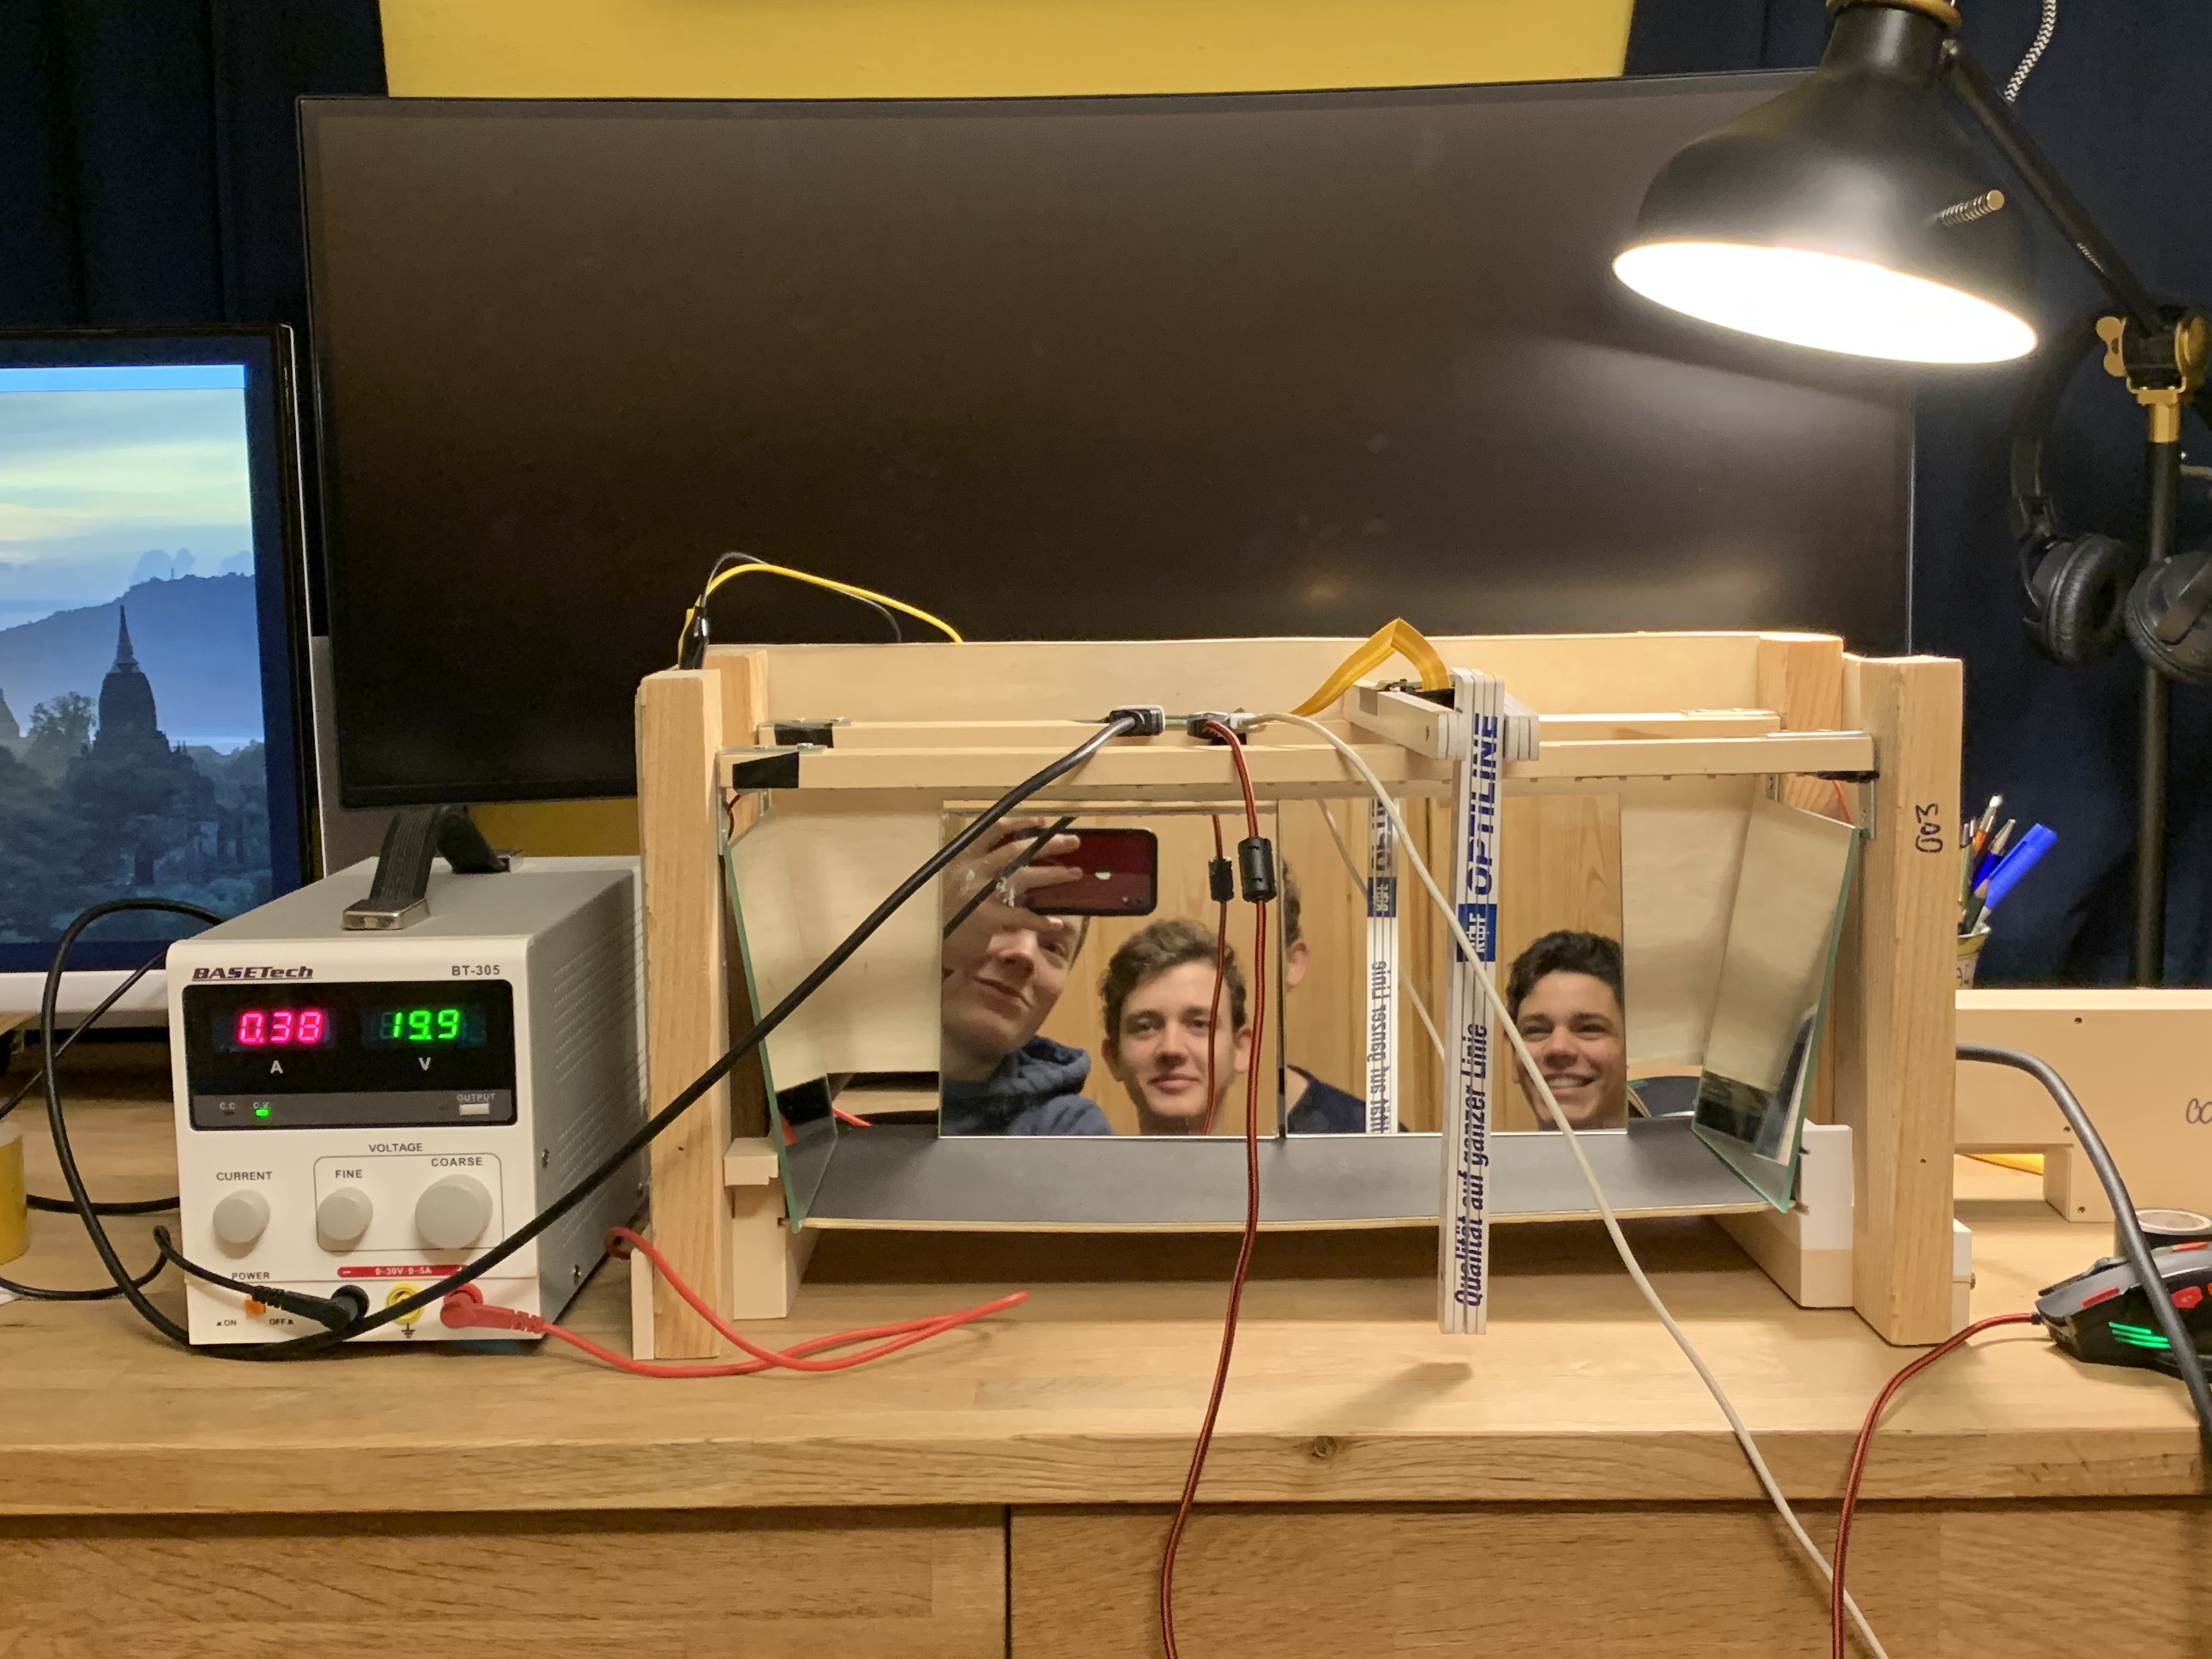
\includegraphics[width=.8\textwidth]{images/Gruppe Semi.jpg}
    \caption{Bau der zweiten Generation an Prototypen\\
    \textit{Quelle: Eigenarchiv}}
\end{figure}

\begin{figure}[H] \label{fig:second-generation-on-hive}
    \centering
    \begin{subfigure}{.45\textwidth}
        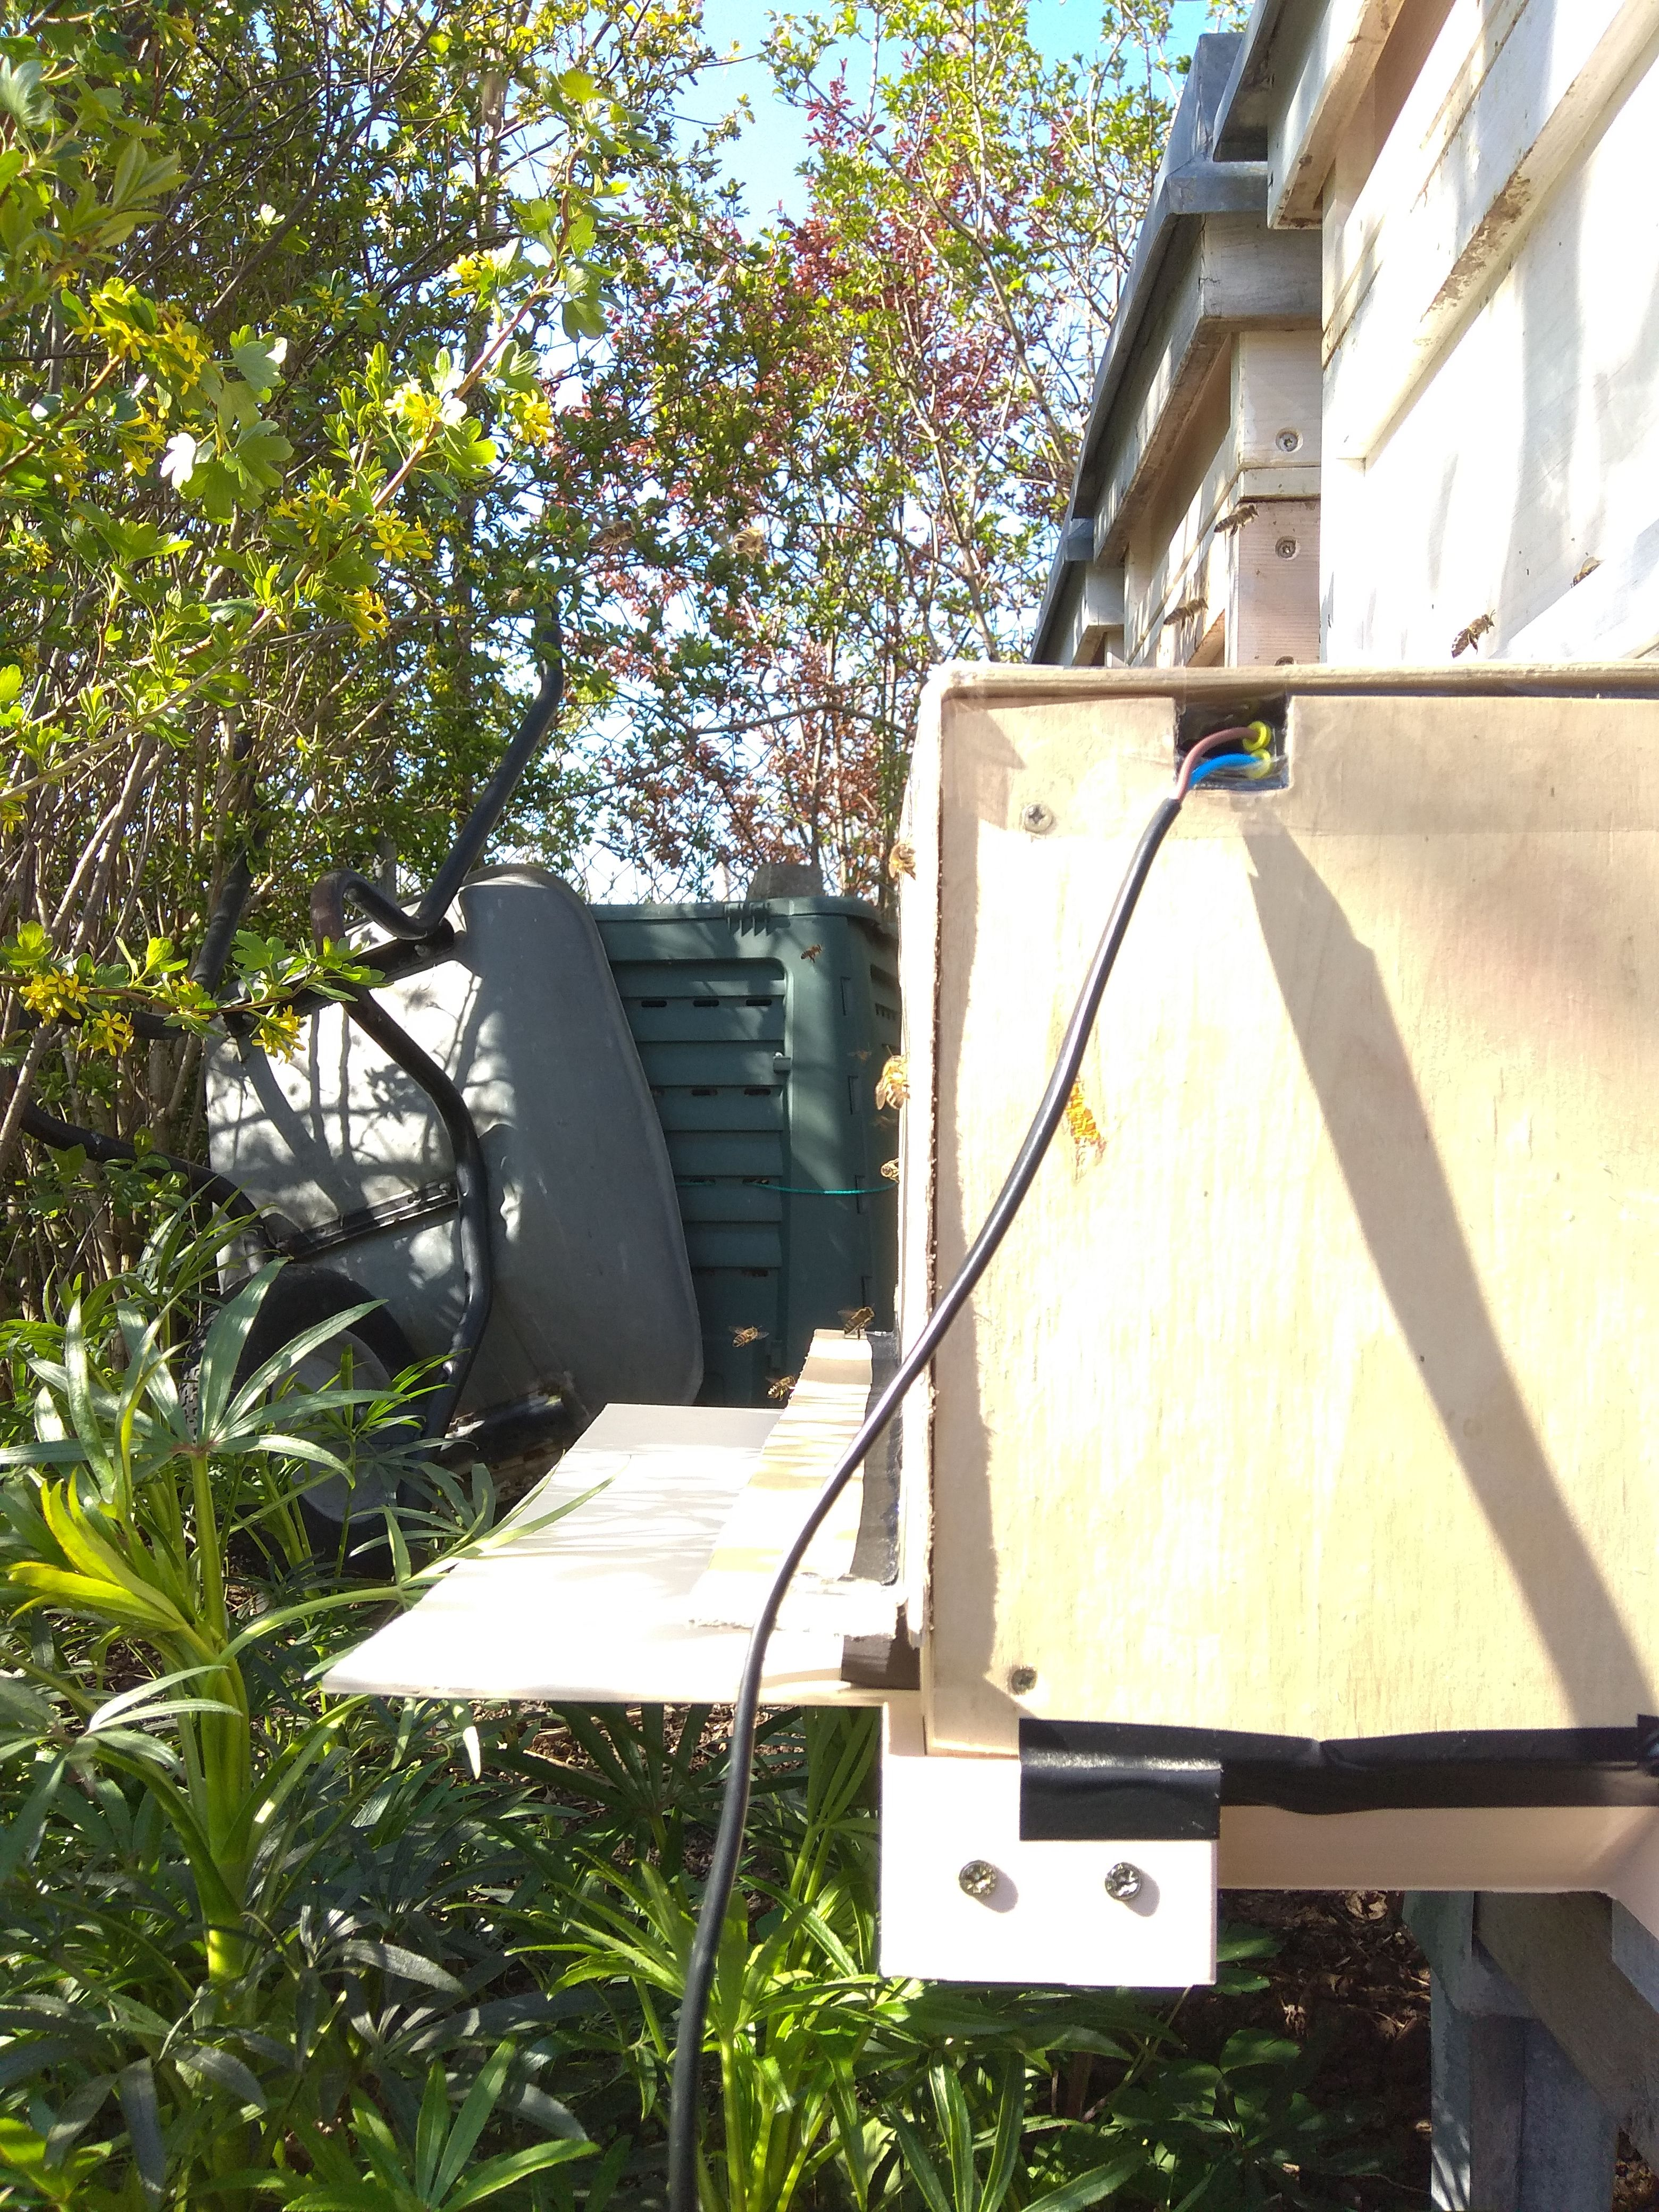
\includegraphics[width=.8\textwidth]{images/second-prototype-on-beehive.jpg}
    \end{subfigure}
    \hfill
    \begin{subfigure}{.45\textwidth}
        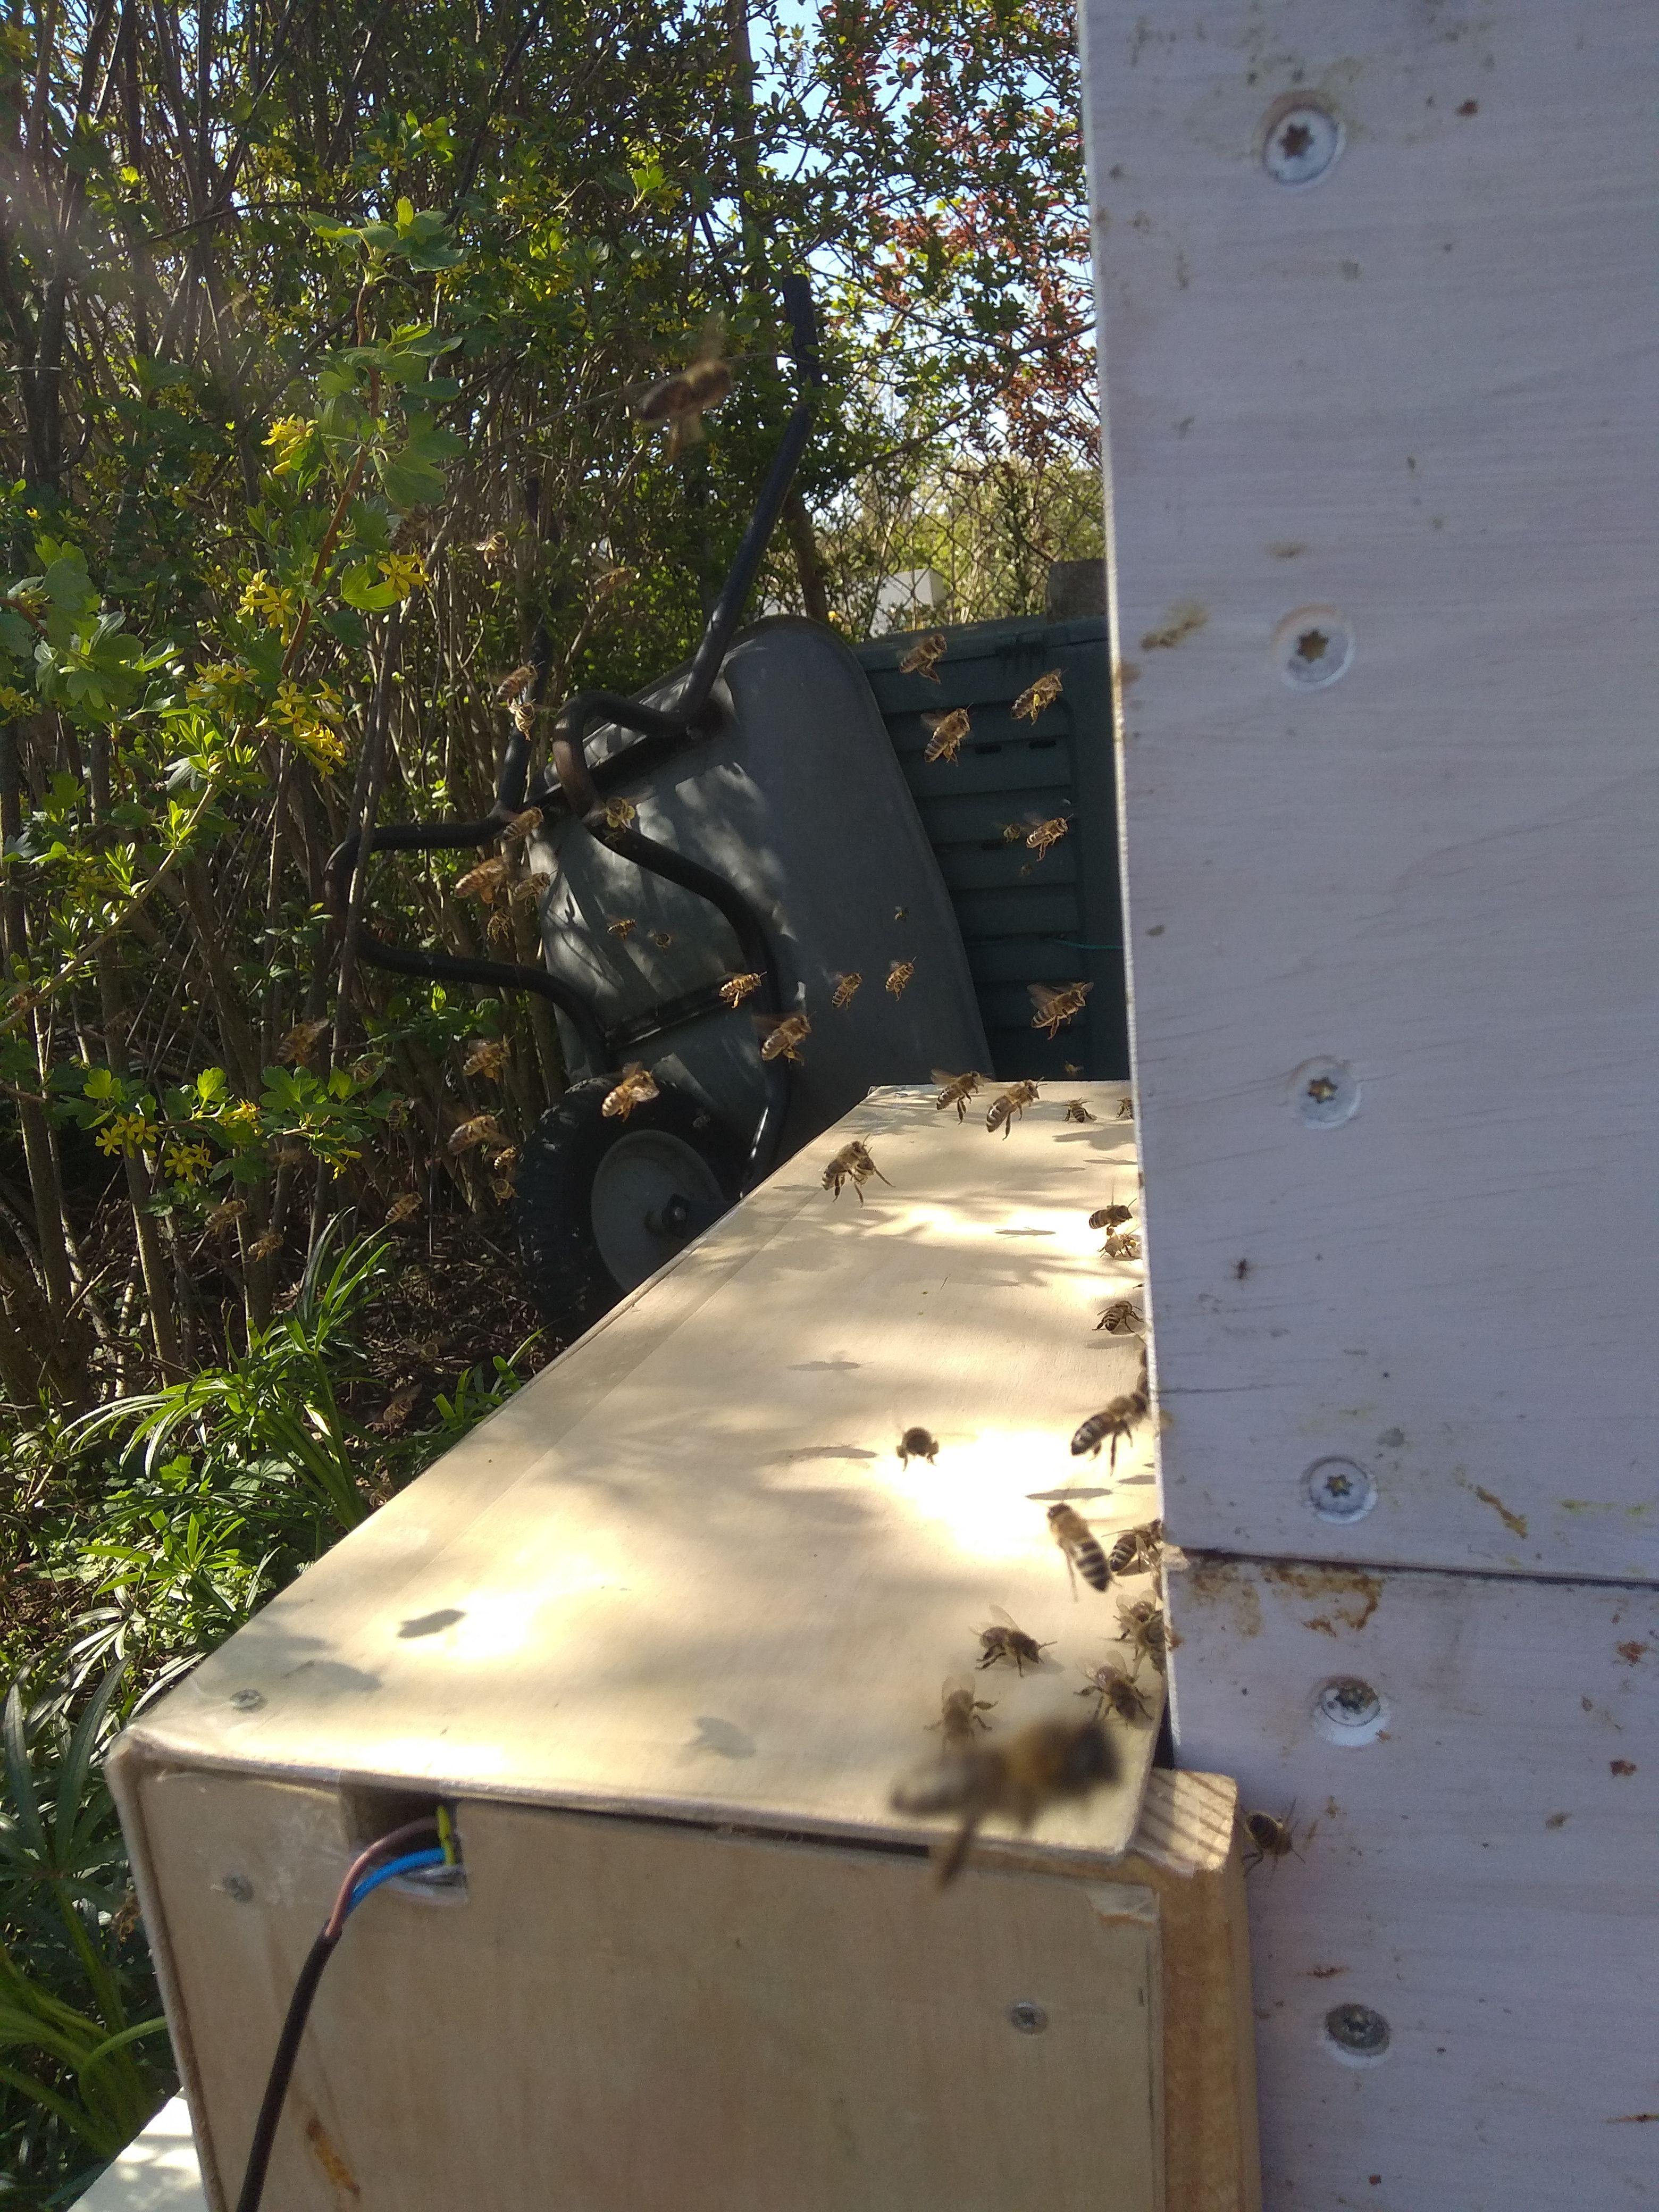
\includegraphics[width=.8\textwidth]{images/second-prototype-problem.jpg}
    \end{subfigure}
    \caption{Problem beim Anbei der zweiten Generation: Bienen finden den Eingang nicht\\
    \textit{Quelle: Eigenarchiv}}
\end{figure}

\begin{figure}[H] \label{fig:third-generation-setup}
    \centering
    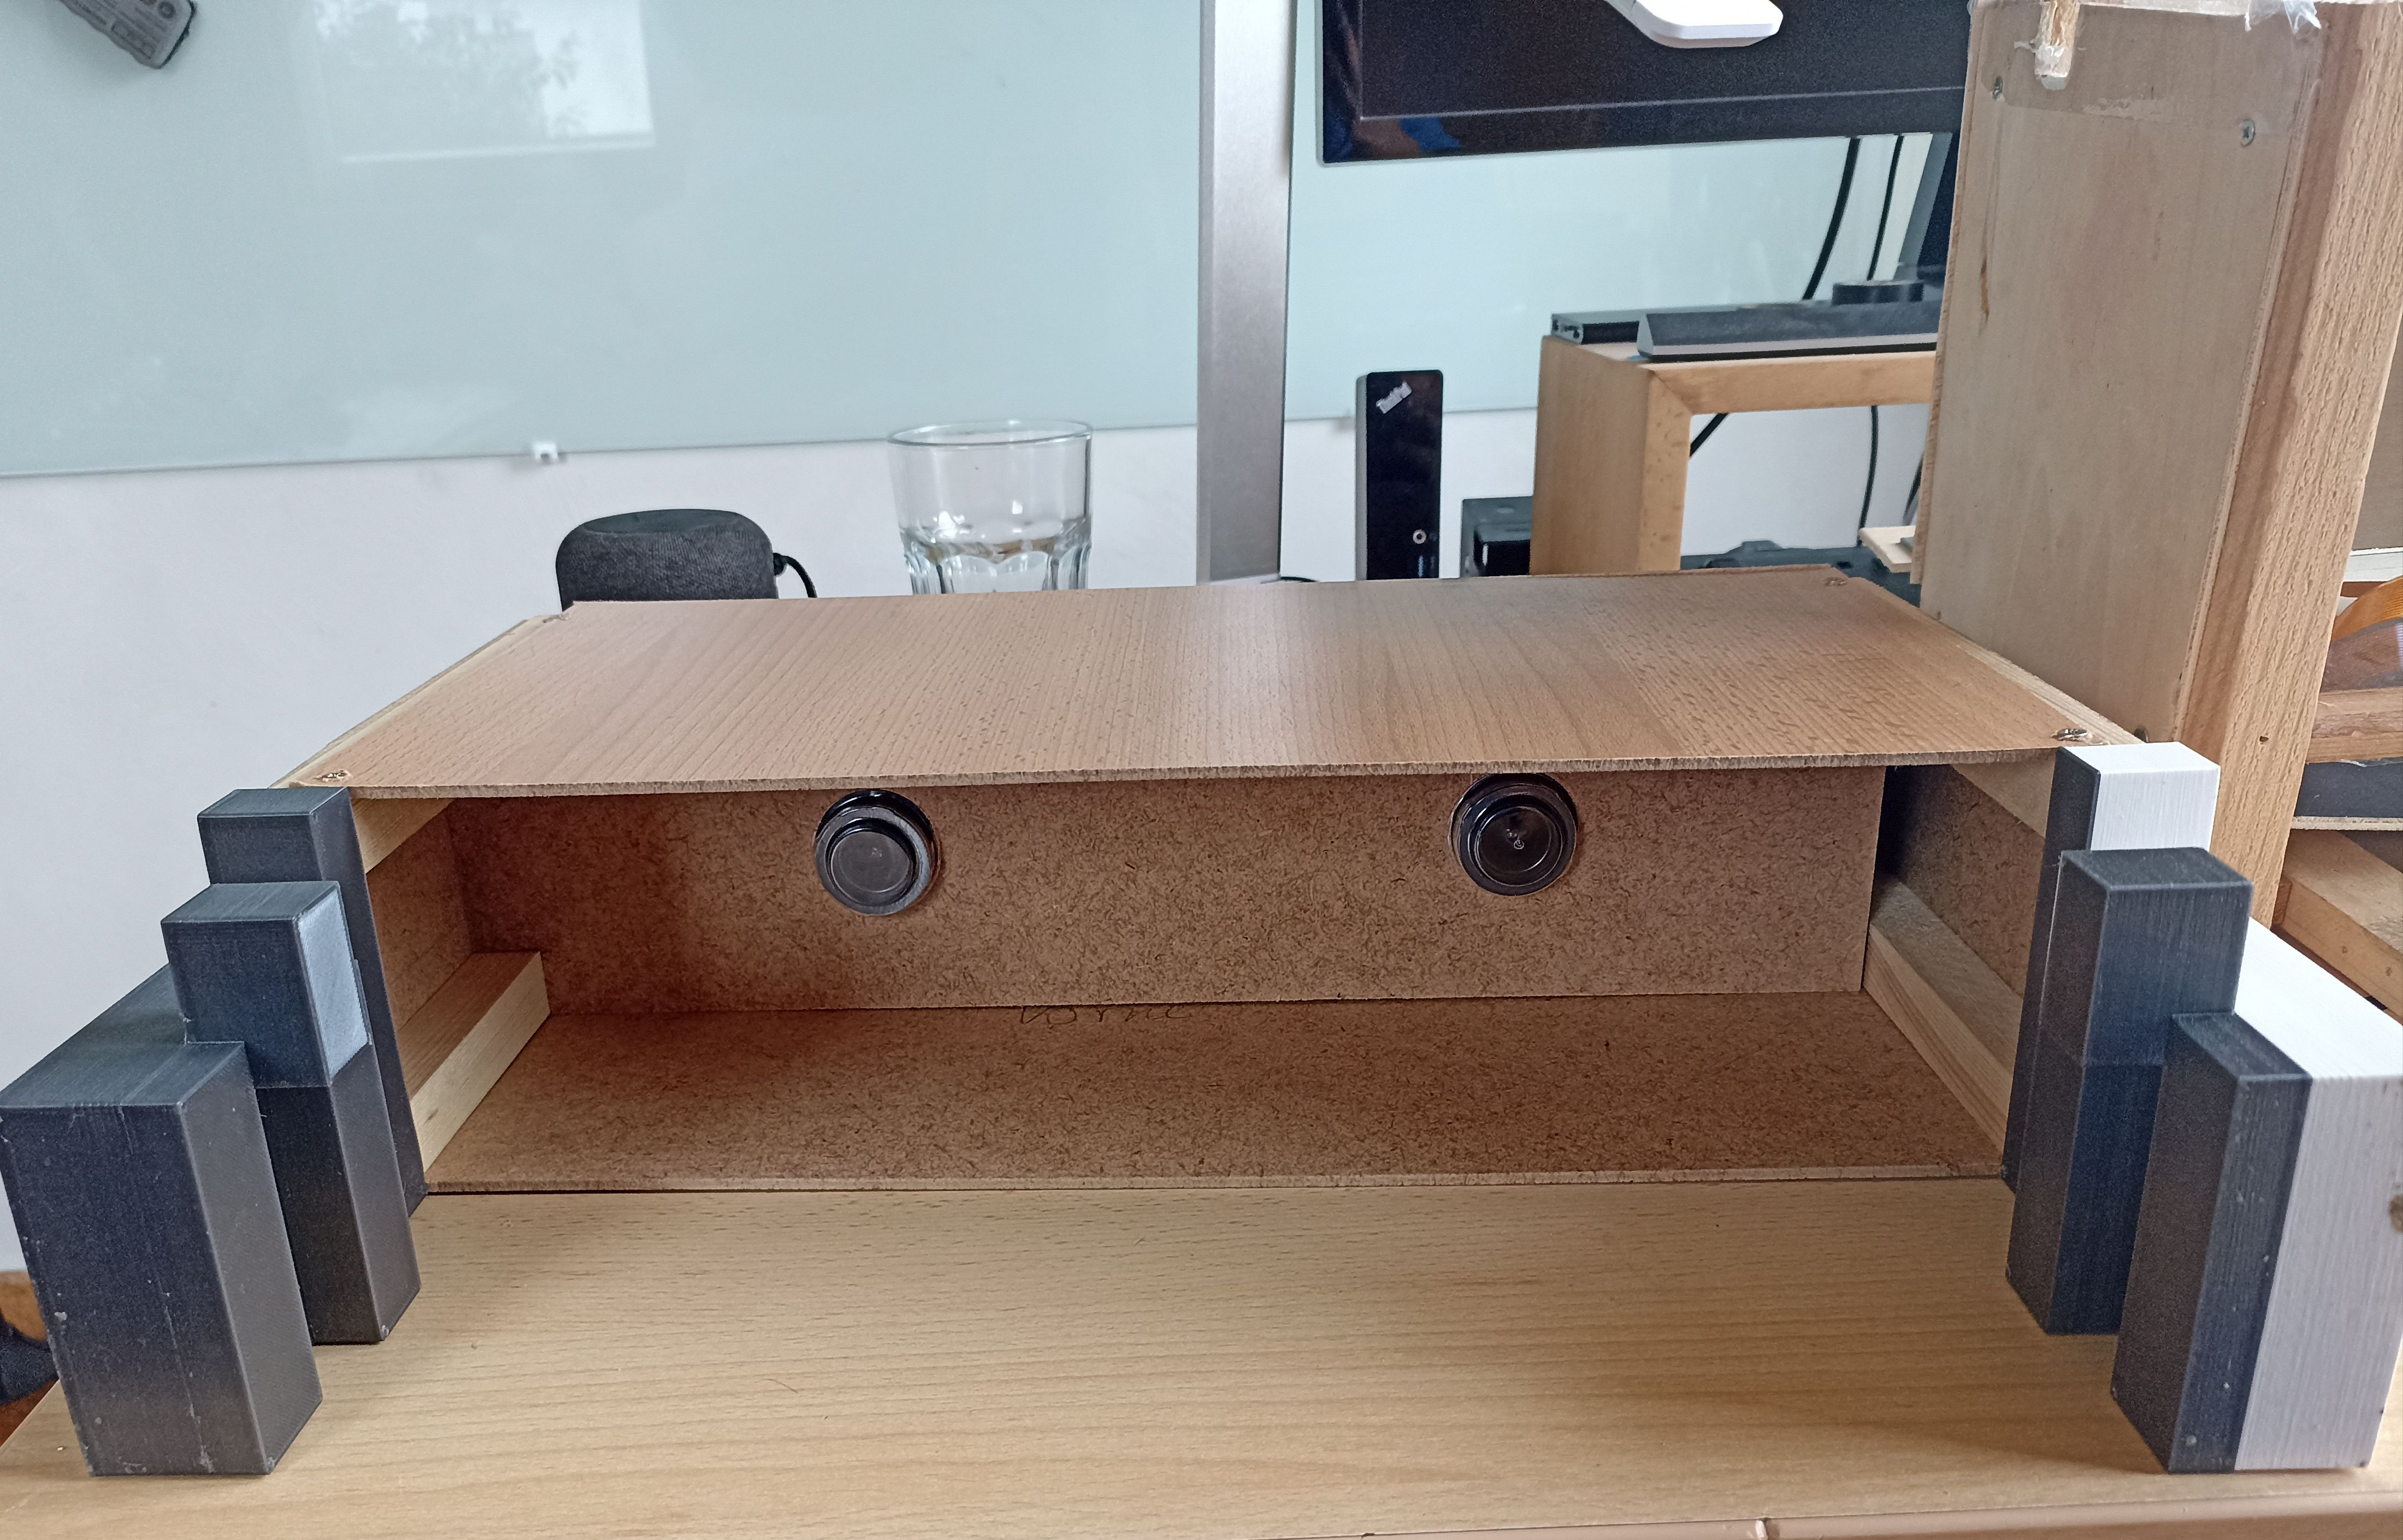
\includegraphics[width=.9\textwidth]{images/third-prototype-electronics-2.jpg}
    \caption{Trennung der Technik von den Bienen in der dritten Generation unserer Prototypen\\
    \textit{Quelle: Eigenarchiv}}
\end{figure}

\begin{figure}[H] \label{fig:third-generation-electronics}
    \centering
    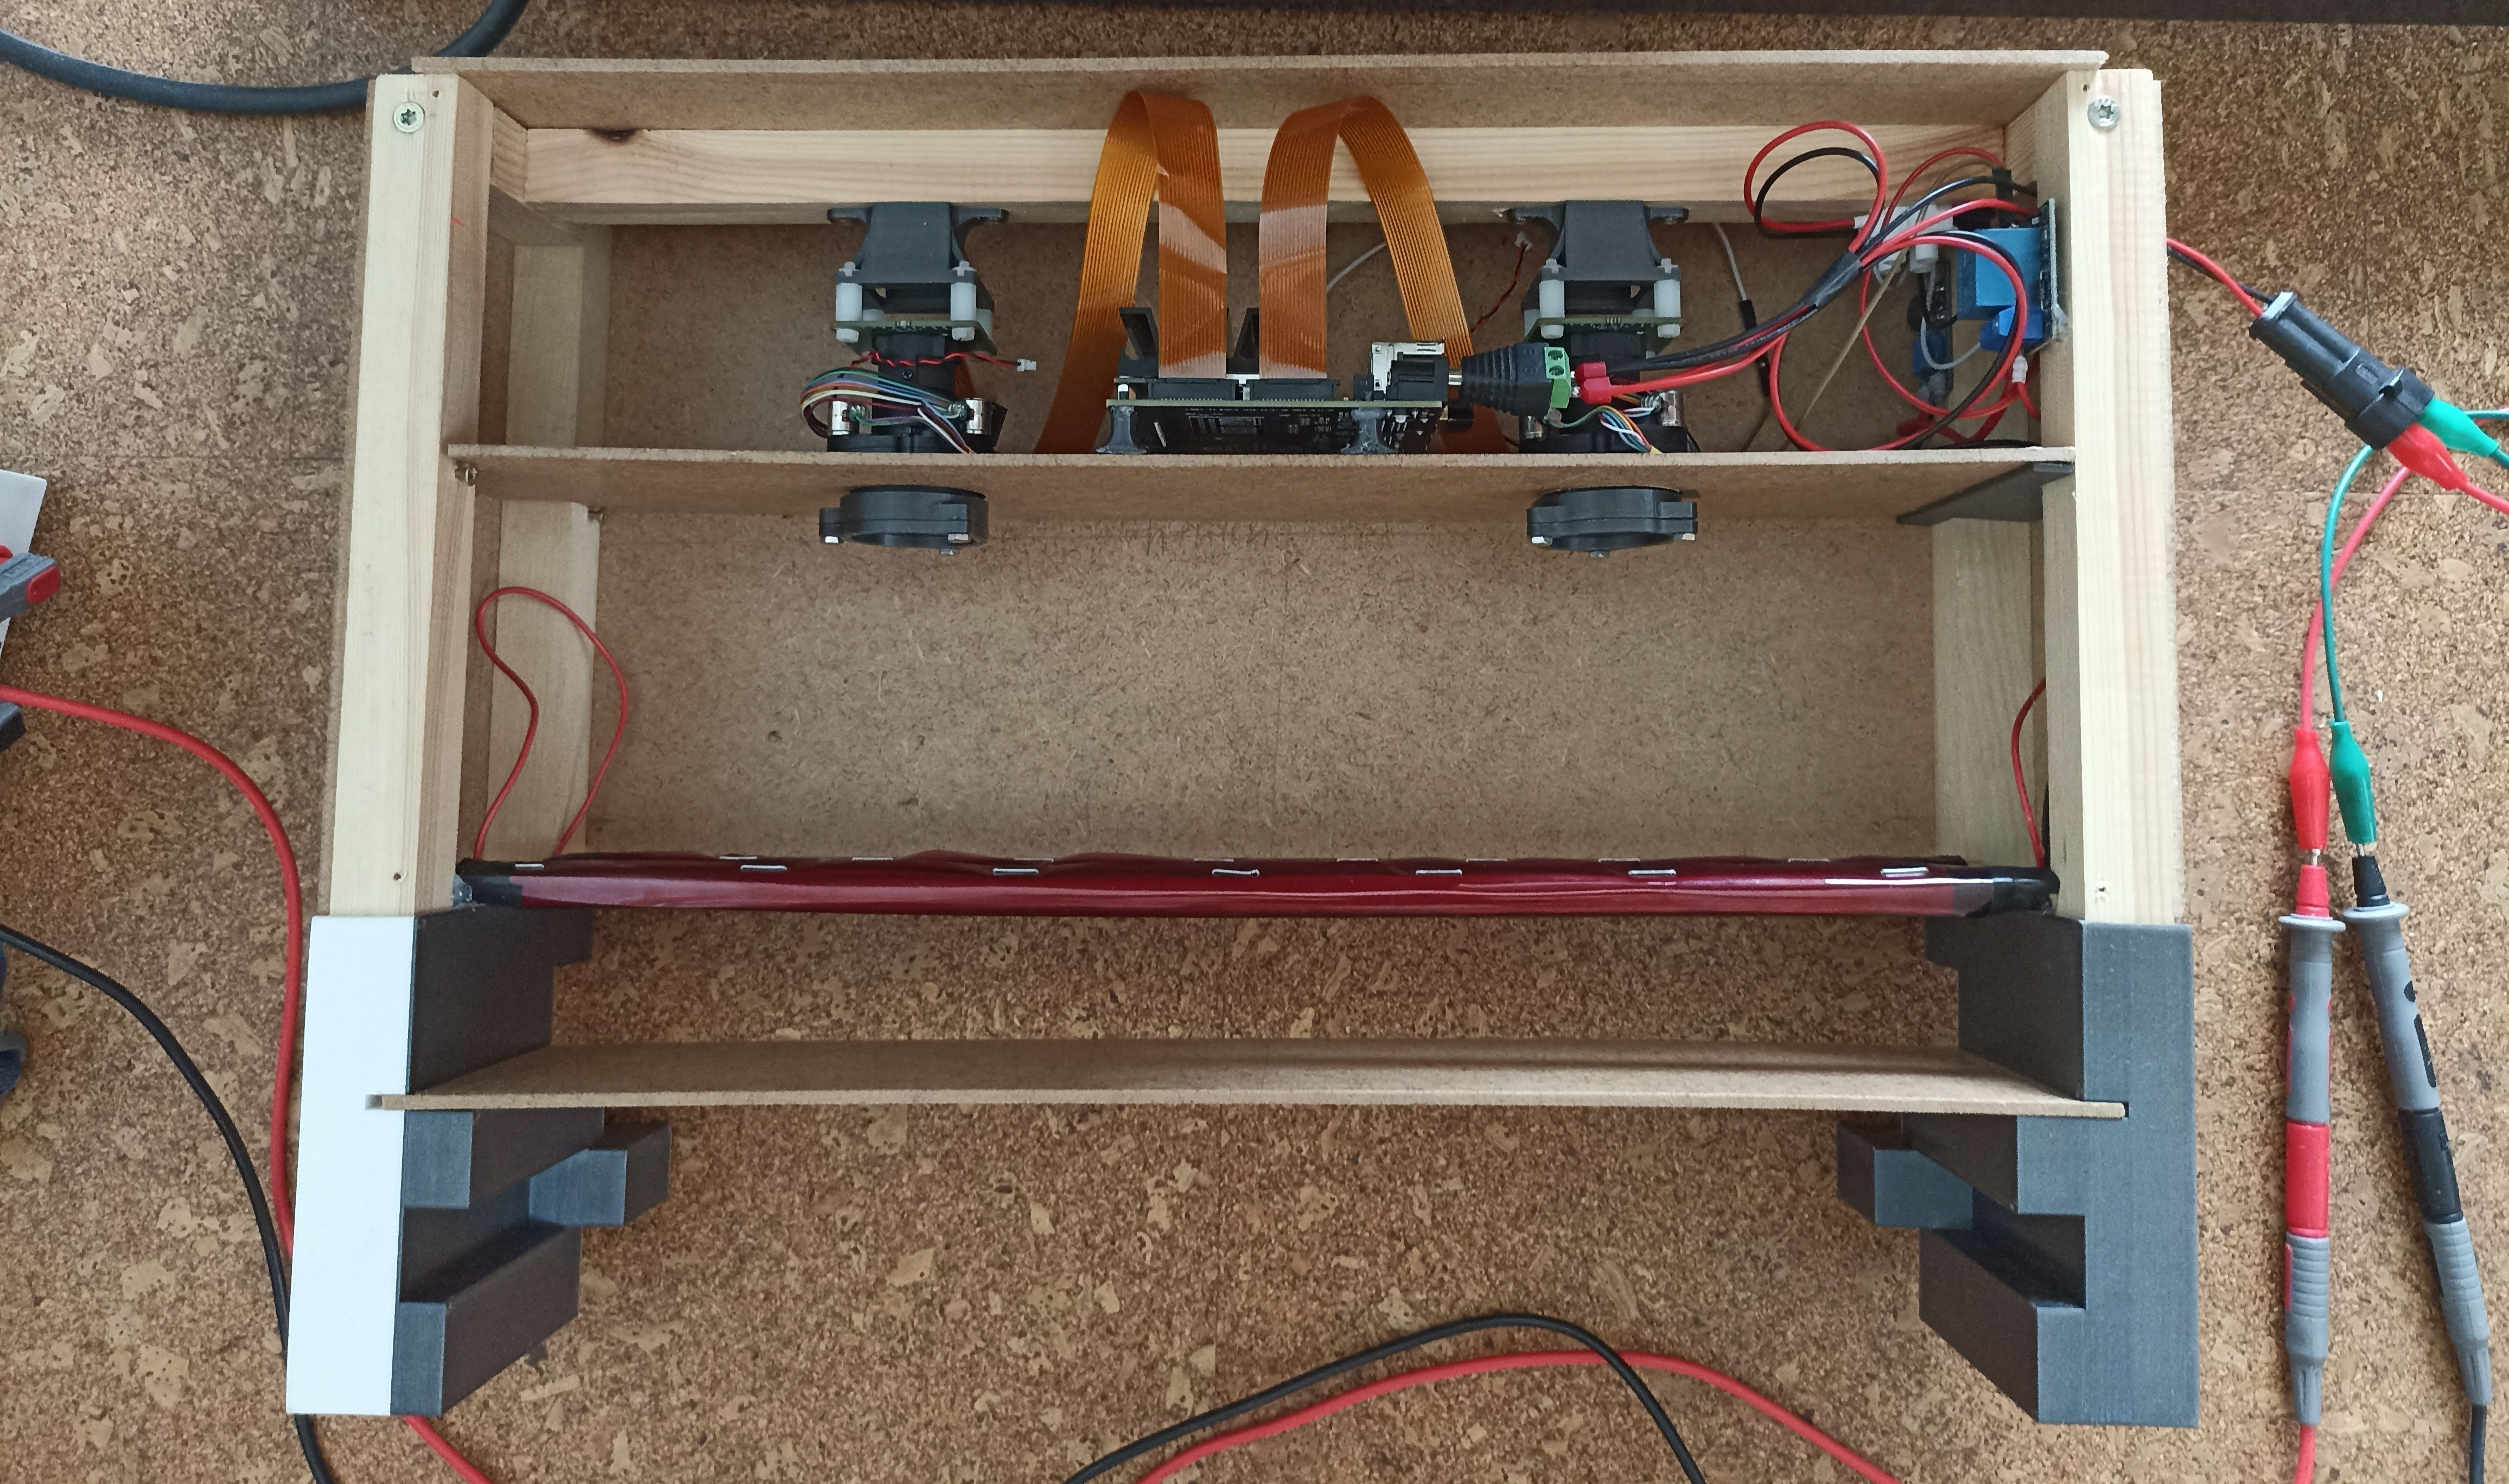
\includegraphics[width=.9\textwidth]{images/third-prototype-electronics-1.jpg}
    \caption{Die Elektronik des dritten Prototyps \\
    \textit{Quelle: Eigenarchiv}}
\end{figure}

\begin{figure}[H] \label{fig:third-generation-on-hive}
    \centering
    \begin{subfigure}{.45\textwidth}
        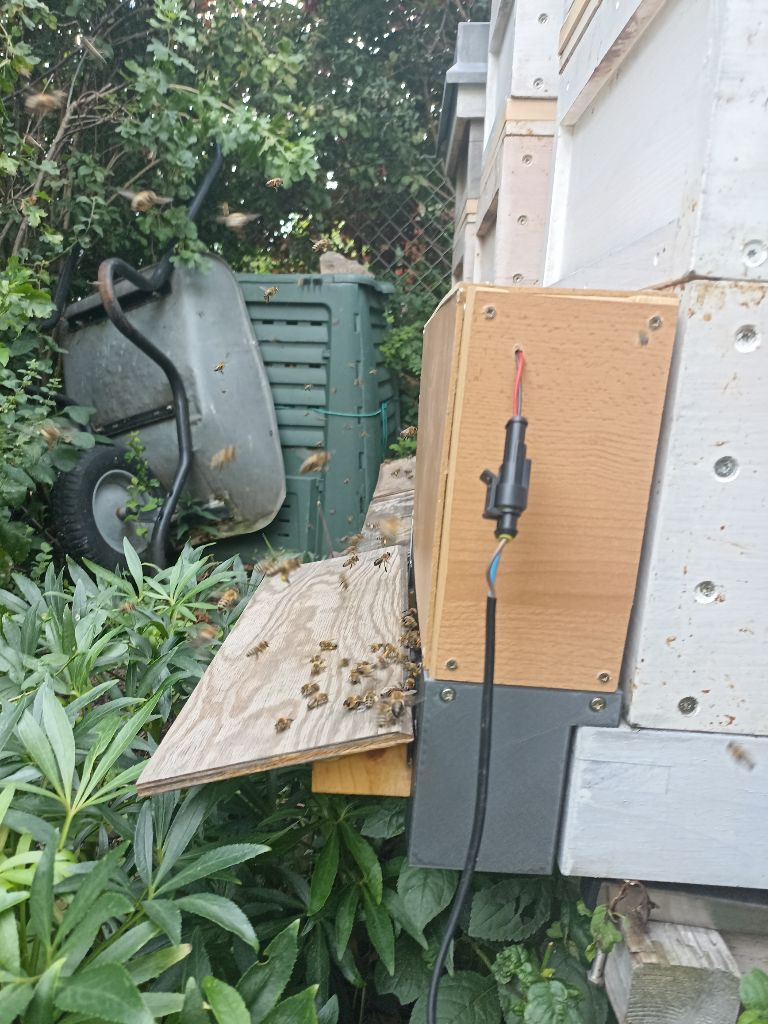
\includegraphics[width=.8\textwidth]{images/thirdPrototype1.jpg}
    \end{subfigure}
    \hfill
    \begin{subfigure}{.45\textwidth}
        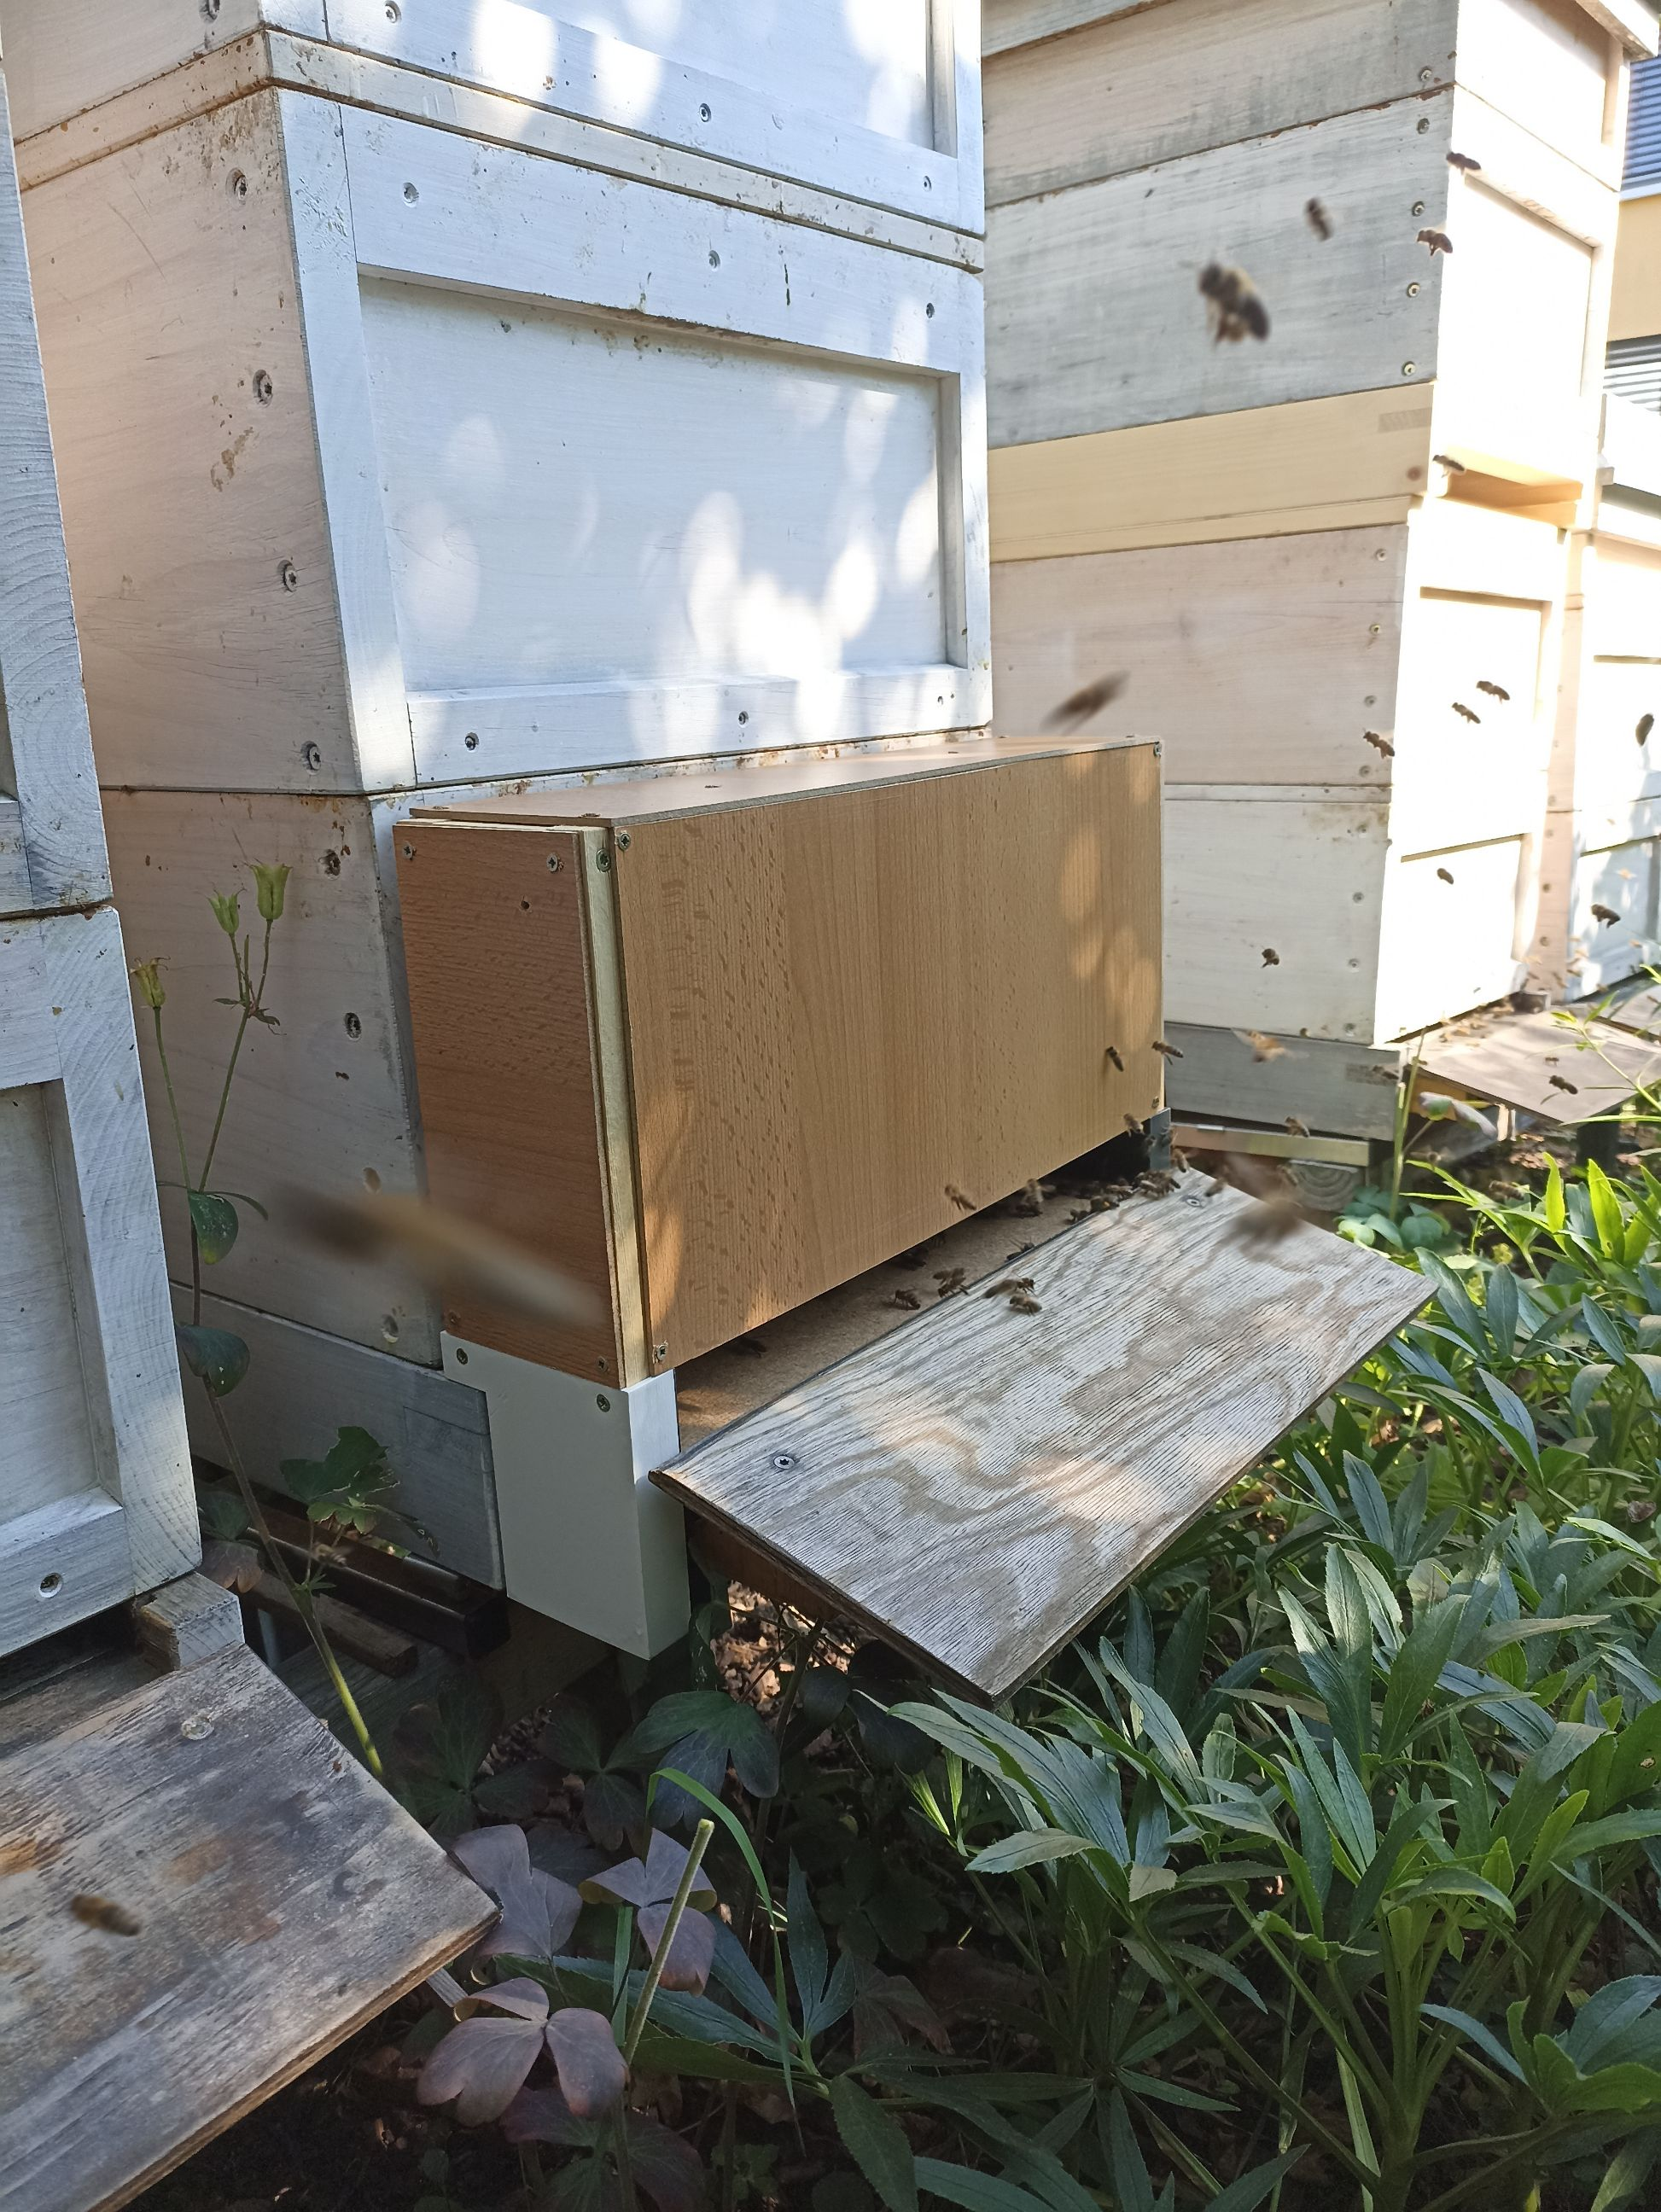
\includegraphics[width=.8\textwidth]{images/thirdPrototype2.jpg}
    \end{subfigure}
    \caption{Der Dritte Prototyp während der Langzeittests \\
    \textit{Quelle: Eigenarchiv}}
\end{figure}

\subsection{Zu Kapitel \autoref{section:Programmierung}}
\begin{figure}[!htb] \label{annotated1}
    \centering
	    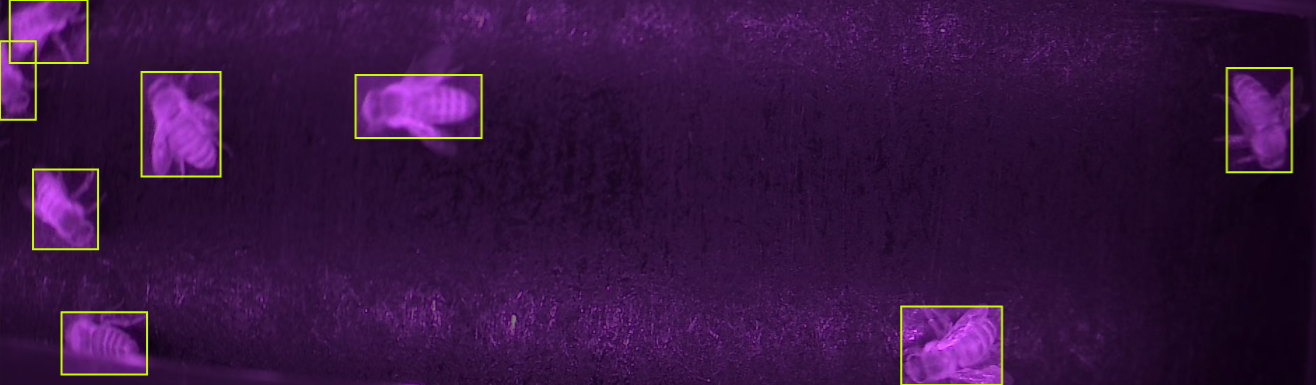
\includegraphics[width = .8\textwidth]{images/annotated1.png}
        \caption{Regelkonform annotiertes Bild}
\end{figure}

\begin{figure}[!htb] \label{annotated2}
    \centering
	    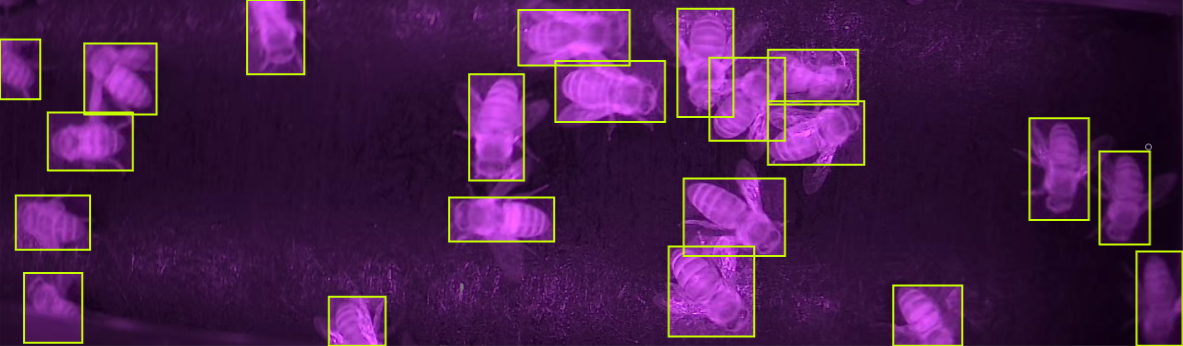
\includegraphics[width = .8\textwidth]{images/annotated2.png}
        \caption{Regelkonform annotiertes Bild}
\end{figure}

\begin{figure}[!htb] \label{annotated3}
    \centering
	    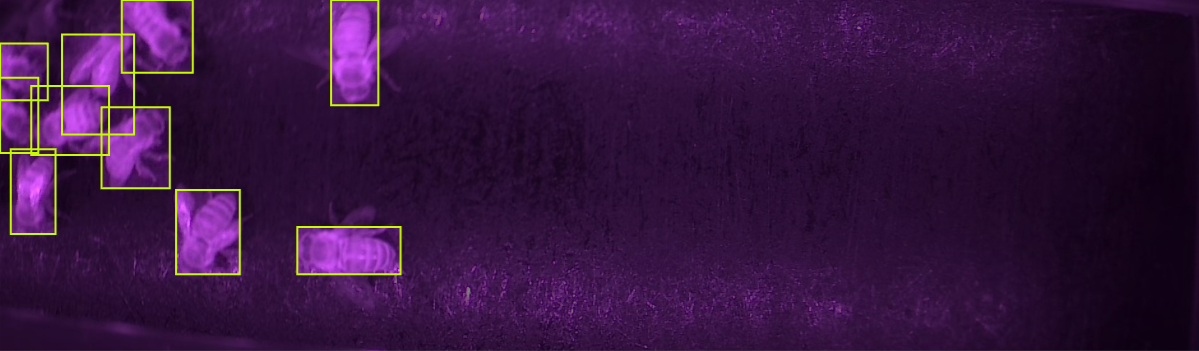
\includegraphics[width = .8\textwidth]{images/annotated3.png}
        \caption{Regelkonform annotiertes Bild}
\end{figure}
% ---------------------------------------
% --------Quellenverzeichnis-------------
% ---------------------------------------
\newpage
\section{Literatur- und Quellenverzeichnis}
\begin{thebibliography}
\\
\subsection{Gedruckte Literatur}

\subsection{Internetliteratur}
\setcounter{enumiv}{0}

\bibitem{br.de}\label{i1}
	\textsc{Autor unbekannt};
	\textit{Die Varroamilbe: Der gefährlichste Feind der Biene}\\
	\url{https://www.br.de/wissen/bienen-varroamilbe-bienensterben-lithiumchlorid-100.html}\\
	letzter Zugriff: 11.10.2021

\bibitem{bee-careful.com}\label{i2}
	\textsc{Autor unbekannt};
	\textit{Warum sind Bienen so wichtig?}\\
	\url{https://www.bee-careful.com/de/initiative/warum-sind-bienen-so-wichtig/}\\
	letzter Zugriff: 11.10.2021

\bibitem{blog.roboflow.com} \bibLabel{annotate-tips}
	\textsc{Nelson, Joseph};
	\textit{Seven Tips for Labeling Images for Computer Vision}\\
	\url{https://blog.roboflow.com/tips-for-how-to-label-images/}\\
	letzter Zugriff: 25.6.2021

\bibitem{darknet.com} \bibLabel{darknet-yolov4}
	\textsc{Alexey Bochkovskiy};
	\textit{Darknet releases}\\
	\url{https://github.com/AlexeyAB/darknet/releases}\\
	letzter Zugriff: 25.6.2021

\bibitem{link.springer.com} \bibLabel{wechselwarm}
    \textsc{Harald Esch};
    \textit{Über die Körpertemperaturen und den Wärmehaushalt von Apis mellifica}\\
    \url{https://link.springer.com/article/10.1007/BF00298066}\\
    letzter Zugriff: 15.12.2021

\bibitem{ssh.com} \bibLabel{ssh}
    \textsc{Tatu Ylonen};
    \textit{SSH (Secure Shell) Home Page}\\
    \url{https://www.ssh.com/academy/ssh}\\
    letzter Zugriff: 17.12.2021
    
\bibitem{udemy.com} \bibLabel{udemy}
	\textsc{Portilla, Jose};
	\textit{Python for Computer Vision with OpenCV and Deep Learning}\\
	\url{https://www.udemy.com/course/python-for-computer-vision-with-opencv-and-deep-learning/}\\
	letzter Zugriff: 23.04.2021

\bibitem{kompendium.infotip.de} \bibLabel{compression}
	\textsc{Autor unbekannt};
	\textit{Videokompression Grundlagen}\\
	\url{https://kompendium.infotip.de/grundlagen_videokompression.html/}\\
	letzter Zugriff: 17.09.2021

\bibitem{beeventure.de} \bibLabel{flugloch}
    \textsc{Karl Weiß};
    \textit{Flugloch}\\
    \url{http://www.beeventure.de/imkerei/beuten/flugloch.html}\\
    letzter zugriff: 18.12.2021

\bibitem{nvidia.com} \bibLabel{jetson-nano}
    \textsc{Autor Unbekannt};
    \textit{NVIDIA Jetson Nano}\\
    \url{https://www.nvidia.com/de-de/autonomous-machines/embedded-systems/jetson-nano/}\\
    letzter Zugriff: 18.12.2021

\bibitem{businessinsider.de} \bibLabel{protoyping}
    \textsc{Autor Unbekannt};
    \textit{Prototyping}\\
    \url{https://www.businessinsider.de/gruenderszene/lexikon/begriffe/prototyping/}\\
    letzter Zugriff: 19.12.2021

\end{thebibliography}

\end{document}